%%%evan/s comparison plot 
%%%%%%%%%%%%%%%%%%%%%%%%%%%%%%%%%%%%%%%%%%%%%%%%%%%%%%%%%%%%%%%%%%%%%%%%%%%%%
%%%% Preamble
%%%%%%%%%%%%%%%%%%%%%%%%%%%%%%%%%%%%%%%%%%%%%%%%%%%%%%%%%%%%%%%%%%%%%%%%%%%%%

%%%% The uwthesis.sty file relies on the memoir class!
%%%% You should be using the memoir class anyway; it makes life easier:
%%%% http://www.ctan.org/tex-archive/macros/latex/contrib/memoir/
\def\bbbar{\ensuremath{\mathrm{b\bar{b}}}}
\def\ccbar{\ensuremath{\mathrm{c\bar{c}}}}
\newcommand{\PZ}{Z}
\newcommand{\ZZ}{ZZ}
\newcommand{\WW}{WW}
\newcommand{\WZ}{WZ}
\newcommand{\pp}{\Pp\Pp\xspace}
\newcommand{\Wjets}{\ensuremath{\PW+\text{jets}}\xspace}
\def\Wmnbb{\ensuremath{\mathrm{W}(\Pgm\cPgn)+\bbbar}}
\def\WmnH{\ensuremath{\mathrm{W}(\Pgm\cPgn)\mathrm{H}}}
\def\Wbb{\ensuremath{\mathrm{W+\bbbar}}}
\def\hbb{\ensuremath{\mathrm{W+h\rightarrow\bbbar}}}
\def\Wc{\ensuremath{\mathrm{W+c}}}
\def\Wmn{\ensuremath{\mathrm{W}\rightarrow \mu\nu}}
\def\Wln{\ensuremath{\mathrm{W}\rightarrow \ell\nu}}
\def\Wcc{\ensuremath{\mathrm{W+\ccbar}}}
\def\Zll{\ensuremath{\mathrm{Z\rightarrow\ell\ell}}}
\def\MT{M_\mathrm{T}}
\def\ET{$E_\mathrm{T}$}
\def\pt{p_\mathrm{T}}
\def\GeV{\mathrm{GeV}}
\def\TeV{$\mathrm{TeV}$}
\def\tev{$\mathrm{TeV}$}
\def\PYTHIA{$\mathtt{PYTHIA}$}
\def\POWHEG{$\mathtt{POWHEG}$}
\def\MADGRAPH{$\mathtt{MADGRAPH}$}
\def\GEANTfour{$\mathtt{GEANT4}$}
\def\TAUOLA{$\mathtt{TAUOLA}$}
\def\La{\mathscr{L}}
\def\fbinv{fb^\mathrm{-1}}
\def\Pg{\mathrm{g}}
\def\Pp{\mathrm{p}}
\def\Pgt{\mathrm{\tau}}
\def\Pgm{\mathrm{\mu}}
\def\Pe{\mathrm{e}}
\def\cPZ{\mathrm{Z}}
\def\PW{\mathrm{W}}
\def\pt{\mathrm{p_{T}}}
\def\cPqt{\mathrm{q}}
\def\cPaqt{\mathrm{\bar{q}}}%%%%%CHECK THIS
%\def\Pg{$\mathrm{g}$}
%\def\vecEtm{\overline{\slash{E_{T}}}}
%\def\vecPtmu{\overline{p_{T}(\mu)}}
%\def\MET{\slash{E_{T}}}
\def\ttbar{\ensuremath{t\bar{t}}}
\def\vecEtm{\ensuremath{\vec{E}_\mathrm{T}^{\mathrm{miss}}}\;}
\def\MET{\ensuremath{E_\mathrm{T}^{\mathrm{miss}}}\;}
\def\vecPtmu{\ensuremath{\vec{P}_\mathrm{T}^{\mu}}\;}

\newcommand{\Lint}{\ensuremath{{\cal L}_{\mathrm{int}}}}
\newcommand{\dytt}{\ensuremath{\cPZ/\Pgg^*\to\tau^+\tau^-}}
\newcommand{\dyll}{\ensuremath{\cPZ/\Pgg^*\to \ell^+\ell^-}}
\newcommand{\stat}{\ensuremath{\,\mathrm{(stat.)\;}}}
\newcommand{\syst}{\ensuremath{\,\mathrm{(syst.)\;}}}
\newcommand{\lumi}{\ensuremath{\,\mathrm{(lum.)\;}}}
\newcommand{\theo}{\ensuremath{\,\mathrm{(theo.)}}\;}



\RequirePackage{lineno}
\documentclass[oneside, letterpaper, 12pt, oldfontcommands]{memoir}

%%%% Import uwthesis.sty to get official formatting, then set your variables.
\usepackage{uwthesis}
\usepackage{graphicx}
\usepackage{mathtools}
\usepackage{subcaption}
\usepackage{graphicx}
\usepackage{caption}
\usepackage{subcaption}
\usepackage{amsfonts}
\usepackage{mathrsfs}
\usepackage{amsmath}
\usepackage{adjustbox}
%\usepackage[sorting=none]{biblatex}

%Search for an MSSM Higgs Boson and Measurement of W+b b
%with the CMS Detector at the LHC.
\settitle{
Search for an MSSM Higgs Boson and Measurement of W+ $b\bar{b}$
with the CMS Detector at the LHC}
\setauthor{Isobel Rose Ojalvo}
\setdepartment{Physics}
\doctors % or \masters
\setgraddate{2013}
\setdefensedate{11 February 2013} % or whatever format you want

%%%% Members of the Final Oral Committee (FOC)
%%%% Give name, rank, and department
%%%% 
\setfoca{Wesley Smith}{Bjorn Wiik Professor}{Physics} % <- Your advisor
\setfocb{Sridhara Dasu}{Professor}{Physics}
\setfocc{Lisa Everett}{Professor}{Physics}
\setfocd{Matthew Herndon}{Professor}{Physics}
\setfoce{Terry Millar}{Professor}{Mathematics}


%%%% Your abstract, used for the UMI abstract and in your front matter
\setabstract{%
This thesis describes a standard model cross section measurement of $\Wbb$ 
as well as a search for neutral Higgs bosons in the minimal supersymmetric 
extension of the standard model (MSSM) decaying to tau pairs.

The measurement of $\Wbb$ was performed
using proton-proton
collisions at $\sqrt{s} = 7~\mathrm{TeV}$ in a data sample collected
with the CMS experiment at the LHC corresponding to
an integrated luminosity of  $5.0~\mathrm{fb}^{-1}.$
The $\mathrm{W+b\bar{b}}$
events are selected in the $\mathrm{W}\rightarrow\mu\nu$ decay mode by requiring a
muon with transverse momentum $p_{\mathrm{T}}>25~\mathrm{GeV}$ and pseudorapidity
$|\eta|<2.1$, and exactly two b-tagged jets with $p_{\mathrm{T}}>25~\mathrm{GeV}$ and $|\eta|<2.4$.
The measured $\mathrm{W+b\bar{b}}$ production cross section in the fiducial region, calculated at the level of final-state particles, is
$0.53\pm 0.05~(\textrm{stat.}) \pm 0.09~(\textrm{syst.}) \pm 0.06~(\textrm{th.}) \pm 0.01~(\textrm{lum.}) ~\textrm{pb}$,
in agreement with the standard model prediction. 
This measurement serves as an important
benchmark at the LHC especially to 
searches which include a single, isolated lepton and one or more b jets in the final state,
as $\Wbb$ is an irreducible background.

The search for neutral Higgs bosons in their decay to tau pairs is performed 
using events recorded by the CMS experiment at the LHC
in 2011 and 2012 at a center-of-mass energy of 7 TeV and 8 TeV respectively. 
The dataset corresponds to an integrated luminosity of 24.6~fb$^{-1}$, 
with 4.9~fb$^{-1}$ at 7 TeV and 19.7 fb$^{-1}$ at 8 TeV. To enhance 
the sensitivity to neutral MSSM Higgs bosons, the search
 includes the case where the Higgs boson is produced in association 
 with a b-quark jet. No excess is observed in the tau-pair invariant-mass 
 spectrum. 
 %Exclusion limits in the MSSM parameter space of $M_A$ 
 %and tan$\beta$ in the $m_h^{\rm max}$ scenario are presented. 


}

%%%%%%%%%%%%%%%%%%%%%%%%%%%%%%%%%%%%%%%%%%%%%%%%%%%%%%%%%%%%%%%%%%%%%%%%%%%%%
%%%% Document
%%%%%%%%%%%%%%%%%%%%%%%%%%%%%%%%%%%%%%%%%%%%%%%%%%%%%%%%%%%%%%%%%%%%%%%%%%%%%

\begin{document}
%%%%%%SETLINE NUMBERS
%\setpagewiselinenumbers
\modulolinenumbers[1]
\linenumbers
%%%%%%END SETLINE NUMBERS
% Tell the memoir class to set up lowercase roman for pagination, etc.
\frontmatter

%%%% Uncomment this to create a UMI abstract page.
%%%% If you are submitting electronically, however, this page is unnecessary.
% \theumiabstract

% The title page
\thetitlepage
\clearpage

% The copyright page, if you want to pay the fee and register copyright.
\thecopyrightpage
\cleardoublepage

% These above pages should not be counted, so we reset the counter to 1.
\setcounter{page}{1}

% An abstract may be required by your department.
\section{Abstract}
\uwabstract
\cleardoublepage

% Acknowledgements go here if you want to include them.
\section{Acknowledgements}
This is where any acknowledgements would go.
\clearpage

% Table of contents
\maxtocdepth{subsection}
\tableofcontents* % the * means that there isn't an entry for the TOC itself
% \clearpage
 \listoffigures*  % if you have any figures
% \clearpage
 \listoftables   % if you have any tables

% Tell the memoir class to set up normal pagination, etc. for the main doc
\mainmatter

\chapter{The Standard Model}
\section{A Historical Approach to High Energy Physics}
 In 450 B.C. the greek philosopher Democritus created the term "atom"
 to refer to an indivisible quanta of which all matter is composed.
While Democritus' use of this word was purely philosophical,
scientific study of the building blocks of matter began in the late 19th
 century. The first leap forward in understanding of the field of
 particle physics came in 1897 J. J. Thomson fired "cathode rays" into a magnetic field. 
He observed their circular orbit in this magnetic field and by measuring
the radius of the orbit, Thomson
 was able to make the first measurement of the electron mass.
 Thomson already knew these electrons were in some way associated
 to the atom; he hypothesized that the electrons were distributed
 evenly with in the atom, much like frogs floating in a pond.
 In 1899 Rutherford tested this hypothesis by firing a beam of 
 $\alpha$-particles at a thin gold sheet. He observed that most of the
 $\alpha$-particles went straight through the sheet, but a few bounced
 off in various directions; this suggested that the $\alpha$-particles were made mostly of 
 space with an indivisible nucleus that would on occasion interact and
 cause the scattering. Rutherford named the nucleus of the lightest
 atom the "proton". Even if at this time physicists had an idea of the nature%fix
 of the most simple of atoms the relationship between the nucleus and the
 electrons was still not well understood. In 1914 Niels Bohr successfully
 developed a model of the Hydrogen atom by approximating the electron
 as a planet circling the Sun, i.e. the nucleus. This equation, %%%insert eqn for bohr hypothesis
Bohr developed, amazingly, was very accurate in determining the 
Hydrogen spectrum. 

Around the same time that Rutherford was measuring the mass of the
electron, Planck found that by quantizing electromagnetic radiation by
$E=h\nu$ he could escape the ultraviolet catastrophe.%%%%fix this what is UV catastrophe?
In 1905 Einstein took Planck's idea of the quantization of the electromagnetic
radiation a step further and claimed that radiation is intrinsically quantized.
%%addequation
This "photoelectric effect" was long rejected by the physics community until
decisively proven by Compton Scattering.
%Dirac discovery of positron
In the 1930's during the study of nuclear $\beta$ decay a problem was
observed. In $\beta$ decay a nucleus transforms into a slightly lighter
nucleus with the emission of an electron; if the neutron is at then the
electron and proton must emerge back to back with equal and opposite
momenta. However, when the energy of the electron was recorded over
many experimental iterations it was shown to vary. A solution to this was
proposed by Pauli that a neutral particle carries off this missing energy; today
this process is known to be $n\rightarrow p^{+}+e^{-}+\bar{\nu}$. 

By this time it had been seen that in any interaction charge and energy
must be conserved% mu- to e- + photon never observed mu = 
%%%%%%%%gluon
%At the time of this measurement, electron-positron experiments regularly observed two-jet events. They indicate the annihilation of the two incoming particles and the subsequent creation of a quark and an antiquark, both of which result in particle jets. If the energy of the collision is sufficiently large, either the quark or the antiquark can emit excess energy in form of a gluon, which also produces a particle jet in the same plane as the two other jets. Only at high energies, the gluon jet appears as a distinct third jet.
%Physicists Sau Lan Wu and Georg �Haimo� Zobernig developed and programmed a method to search for such planar three-jet events among the TASSO data. At low collision energies, their searches produced no results. But when DESY�s PETRA accelerator began to produce collisions at 27.4 GeV, they succeeded. A week later, Bj�rn Wiik presented this first event on behalf of the TASSO collaboration at a physics conference in Bergen, Norway. Shortly thereafter, on June 26, 1979, Wu and Zobernig distributed the above figure in their internal TASSO Note No. 84.

Despite many efforts, no one has ever observed a single, individual 
quark. This produced much skepticism in the 1960's and 70's;
to explain this the idea of "quark confinement" was introduced which
said that quarks are always confined within mesons or baryons. 
%add in something about gluons
In the late 1960's physicists at the Stanford Linear Accelerator (SLAC) %%reference SLAC paper FriedmanKendall
performed deep inelastic scattering experiments to study the sub-structure
of the nucleon. By way of firing an electron at a nucleon and measuring the
scattering of the outgoing electron the experimental results hinted that the
nucleon was actually made up of many point-like constituents. These
point-like constituents would eventually be called "partons". 
W. Greenberg proposed that quarks come in 3 colors, red, green and blue,
(which have anti-red, anti-green, and anti-blue partners) and that each 
quark bound state is actually colorless. 

This widespread skepticism about the quark model remained 
widespread until the discovery of the J/$\psi$ particle by separate groups
at SLAC and MIT. This bound $c\bar{c}$ ground and excited states were
shown to be well described by Quantum Chromodynamics (QCD). %%Write which symmetry it follows?

A very unanticipated third generation of lepton, the $\tau$-lepton, was 
discovered at SLAC. Due to its heavy mass (1784 MeV) the lifetime of the $\tau$ is much
shorter than that of the $\mu$; the reconstruction of the $\tau$ is also
more difficult due to it decay both to leptons ($\tau\rightarrow\mu\bar{\nu_{\tau}}\nu_{\mu}$)
and to hadrons, for example $\tau\rightarrow$.%%%%quote tau decay
This discovery of a third lepton generation was unprecedented as there 
had previously been discovered only 2 generations of quarks. However,
in 1977 a %$$\psi???
resonance was observed via its decay to $\mu^{+}\mu^{-}$ at approximately
9.5 GeV. It was later shown that this peak at 9.5 GeV was actually three $b\bar{b}$ resonances.
The b-quark is much more massive than the c-quark; the b-quark's decay and
its huge importance in the discovery of new physics is outlined in section %%%%. 

By 1979 the production of $q\bar{q}$ had already been observed in 
electron-positron collisions at Petra %%check this
via the process $e^{+}e^{-}\rightarrow\gamma\rightarrow q\bar{q}$. 
The observation of a 3-Jet event at %%where?
in 1979 via electron-positron collision was extremely exciting as it
was the first evidence of a high energy quark emitting a gluon via
Bremsstrahlung. This further confirmed QCD and what had started in 201 
%%add in gluons

This summary of observations and hints of the Standard Model confirmation brings us 
to July 2nd 2012 when physicists separately at the CMS and ATLAS 
experiments at CERN both independently reported observation of a 
Higgs-like boson at approximately 125 GeV. In the following sections the
Standard Model (SM) and an extension of this model, the Minimally Supersymmetric
Standard Model (MSSM), is described in more detail. The discovery of a Higgs-like boson
that couples to bosons and fermions is a major milestone in the story
of particle physics. It remains to be seen where the story will go; a search
for the super symmetry is presented with no strong evidence yet to
support this model. However, many important questions about the 
universe remain unanswered and so the saga continues. 
\section{Quarks, Leptons and Gauge Bosons}
Following the advances of the 20th century the fundamental
particles in the SM are composed of 3 generations of quarks and leptons
where each generation has two particles. 

These 6 quarks and 6 leptons
are then mediated by the photon, $\gamma$, the W$^{+/-}$, the gluon

The Standard Model of particle physics follows an %%%
symmetry. As can be seen in figure %%figure
\subsection{The Standard Model}%%%Change name?
The idea that interactions are dictated by symmetry is of central
importance to the formulation of theoretical particle physics. 
Currently, it is the general belief that all particle interactions are
described by local gauge theories and that 
physical quantities (charge, color, lepton number, ect.) are 
always conserved.
To start the description of SM theory we remember that in classical 
mechanics Lagrange's equations of motion are used to
describe the motion of a particle or system of particles. %%ref goldstein
If we consider the generalized coordinates of a system, $q_{i}$,
and it's derivative as a function of time, $\dot{q_{i}}$, the equation
of motion can be written as,
\begin{displaymath}
0=\frac{d}{dt}\left(\frac{\partial L}{\partial\dot{q_{i}}}\right) - \frac{\partial L}{\partial q_{i}}
\end{displaymath}
where $L$ is defined as the difference of the kinetic and the potential energy, $L\equiv T-V$.
This equation equation can be formally extended to act on a wave function with %%I don't like "act on"
continuously varying coordinates $\phi({\bf x},t)$
where {\bf x} is the spatial coordinates and t is time.
In this regime, the Lagrangian equation of motion becomes
\begin{displaymath}
0=\frac{\partial}{\partial x_{\mu}}\left( \frac{\La}{\partial\left(\partial\phi/\partial x_{\mu}\right)}\right)-\frac{\partial\La}{\partial\phi}
\end{displaymath}
In the subsequent sections, following the standard methodology, $\La$ is referred to as the Lagrangian
despite it actually being the Lagrangian density,
\begin{displaymath}
L=\int{\La d^{3}x}.
\end{displaymath}
As was stated in section XXX,%ref StandardModel Section 1
To derive the Lagrangians for the SM we start by stating
the Feynman rules:

\subsection{The Higgs Boson and Electroweak Symmetry Breaking}
\subsection{\bbbar Production at the LHC}


\subsection{Jet Hadronization and b-quarks}%%??
quarks only live for $10^{-15}$ seconds
%FIX jan 9th, references in this chapter as well as comments
\chapter{Supersymmetry and the MSSM}
The standard model performs well in describing experimental observations at energies around
the electroweak scale of $O(246 \GeV)$.
The recent discovery of a standard model-like higgs boson ($m_{h}=$125 GeV) brings with it
more confidence in this theory. 
However, one must explain why the mass of the Higgs boson is as low as 125 GeV whereas
the planck scale is $O(1.22 \times10^{19} \GeV)$
\cite{Martin:1997ns}.
%However, questions arise when this model is seen as 
%a part of a grand unified theory, for example, what happens when we probe
%regions between the electroweak and planck scales $O(1.22 \times10^{19} \GeV)$? 
%The standard model encounters difficulties in renormalization, this is known
%as the Hierarchy Problem
%To illustrate these divergences we consider the radiative corrections to the higgs mass
%from a fermion loop.
%As seen in the previous chapter, 
%The potential of the standard model higgs field can be written as, 
%\begin{equation}
%V= \mu^{2}|\phi|^{2}+\lambda|\phi|^{4}
%\end{equation}
%where $\phi$ is a complex scalar field.
%A non-vanishing vacuum expectation value of $246 \GeV$ is required to derive the masses of the $W/Z$
%and the mass of the higgs which is defined as, $m_{h}=\sqrt{2\lambda v^{2}}$.

\begin{figure}[t]
  \centering
  \begin{subfigure}[trim = 0mm 0mm 0mm 0mm, clip, width=3cm]{.4\textwidth}
	\marginbox{0mm 0pt 0mm 0pt}{\includegraphics[width=\textwidth]{images/fermionLoop.png}}
                %\marginbox{-10mm 0pt 10mm 0pt}{}
                \caption{}
                \label{fig:fermionLoop}
\end{subfigure}
\begin{subfigure}[trim = 0mm 0mm 0mm 0mm, clip, width=3cm]{.4\textwidth}
	\marginbox{0mm 0pt 0mm 0pt}{\includegraphics[width=\textwidth]{images/SLoop.png}}
	\caption{}
                %\marginbox{10mm 0pt -10mm 0pt}{}
                \label{fig:scalarLoop}
                	
  \end{subfigure}
   \caption[]{One loop quantum corrections for a fermion (\ref{fig:scalarLoop}) and a scalar (\ref{fig:scalarLoop}). }
\end{figure}

\section{Motivations for SUSY}
%When considering, for example, higher order radiative corrections to the mass of the higgs. For example, 
A fermion loop correction to $m_{h}$, seen in figure \ref{fig:fermionLoop}, 
%adds the term $-\lambda_{f}\phi \bar{f}f$ to the Lagrangian.
%This 
manifests as a negative-sign correction to the higgs mass, namely,
\begin{equation}
\Delta m_{H}^{2}=-\frac{|\lambda_{f}|^{2}}{8\pi^{2}}\Lambda_{UV}^{2}
\label{eq:SUS1}
\end{equation}
%The loops represent terms which are proportional to $m_{f}^{2}$.
where $\Lambda_{UV}$ is the ultraviolet high-mass cutoff, %%define UV cutoff
therefore, the correction to the higgs mass is large. 
%Then what happens when higher energy scales are considered and $\Lambda_{UV}\rightarrow \infty$?
%Since the standard model is a renormalizable theory one could simply
%pick $\Lambda_{UV}$ so that it regulates the loop. However, this would imply
%that $\Lambda_{UV}$ is the energy scale at which new physics should enter.
%To make matters worse, there are quantum corrections from the radiative
%effects of every particle that couples to the higgs. If each of these 
%particles gain their mass through the higgs mechanism then the entire standard model 
%mass spectrum is sensitive to $\Lambda_{UV}$!
It turns out that the correction due to a scalar loop,
as seen in figure \ref{fig:scalarLoop}, has an opposite sign to that of the fermion loop.
It is quite unnatural that the difference of two large numbers has to be tuned
carefully to obtain the 125 GeV observed Higgs boson mass. 
Supersymmetry supposes that there exists a scalar particle
for every fermion and vice versa. 
Therefore, this theory of symmetry between bosons
and fermions can naturally lead to a low mass higgs. 

%To solve the Hierarchy Problem suppose there exists a massive scalar particle S, 
%of mass $m_{S}$, that couples
%to the higgs with a term $-\lambda_{S}\phi^{2} S^{2}$ as seen is 
%figure \ref{fig:scalarLoop}. This massive scalar would give a correction of,
%\begin{equation}
%\Delta m_{H}^{2}=+\frac{\lambda_{s}}{16\pi^{2}}\left[\Lambda_{UV}^{2} \right].
%\label{eq:SUS2}
%\end{equation}
%By examining (\ref{eq:SUS1}) and (\ref{eq:SUS2}) it is apparent that if each of the quarks
%and leptons is accompanied by a complex scalar with $\lambda_{S}=|\lambda_{f}|^{2}$  %OR TWO??
%then the $\Lambda_{UV}^{2}$ terms will cancel. This model of symmetry between bosons
%and fermions is known as supersymmetry (SUSY).


To define SUSY a set of generators which 
transforms a fermionic state into a bosonic state and vice versa is needed. The simplest 
operator which can perform these operations is a 2 component Weyl spinor $Q$
such that,
\begin{equation}
Q|\mathrm{Boson}\rangle=|\mathrm{Fermion}\rangle \qquad Q|\mathrm{Fermion}\rangle=|\mathrm{Boson}\rangle.
\end{equation}
The generators $Q$ and $Q^{\dagger}$ must obey the anticommutation
and commutation algebra,
\begin{equation}
\{Q,Q^{\dagger}\}=P^{\mu}
\end{equation}
\begin{equation}
\{Q,Q\}=\{Q^{\dagger},Q^{\dagger}\}=0
\end{equation}
\begin{equation}
[P^{\mu},Q ]=[P^{\mu},Q^{\dagger}]=0
\end{equation}
where $P^{\mu}$ is the generator of space-time translations.

In the supersymmetric model the SM and SUSY particles are arranged
into supermultiplets. These supermultiplets must contain both the SM fermion
and the boson superpartner. In the simplest approach, a  spin $\frac{1}{2}$
weyl fermion (for example, $e$) must have %%%check this
a spin-0 superpartner ($\tilde{e}$), likewise, a supermultiplet 
with a spin-1 gauge boson ($W$) would have
 a spin $\frac{1}{2}$ weyl fermion superpartner ($\tilde{W}$).
The naming convention for super particles calls for the names of
the fermionic standard model particles to be prepended by an 's', for example, 
'selectron' is short of 'scalar electron'; the gauge bosons are appended
with an '-ino', for example $\tilde{W}$ is known as a 'wino'. If SUSY remained unbroken
then $m_{e}$ must be equal to $m_{\tilde{e}}$. Since sparticles like $\tilde{e}$ have not 
yet been discovered this implies that SUSY must be a broken
symmetry.

\section{Higgs Sector of the SM}
%%add in an introduction sentence

Electroweak
interactions happen on a very short range ($10^{-14}$ m).
To confine weak interactions to this
short range %fix?
the $W^{\pm}$ and Z bosons must be massive. %%need a transition sentence
However, the lagrangians governing fundamental interactions
of particles are written in terms of gauge symmetries and %fix
 in an unbroken gauge theory the gauge bosons must 
be massless. If one were to simply break the symmetry by adding 
in a mass term then the theory %%fix
would no longer be renormalizeable. Spontaneous Symmetry Breaking (SSB)
breaks the symmetry but still requires that the Lagrangian
is invariant under gauge transformations.  
This can done by introducing a complex $SU(2)_{L}$ doublet scalar
higgs field,
\begin{equation}
\Phi=\left(
    \begin{array}{c}
      \phi^{+} \\
      \phi^{0}
    \end{array}
  \right)
\end{equation}
This two component complex scalar field has four degrees
of freedom, three of them give mass to the $W^{\pm}$ and Z, the fourth
appears as a massive physical particle, the Standard Model Higgs boson. 
The Lagrangian describing interactions with this field is 
\begin{equation}
\La=(D_{\mu}\Phi^{\dagger})(D^{\mu}\Phi) +V(\Phi)
\end{equation}
where $D_{\mu}$ is a covariant derivative
and the scalar potential has the form,
\begin{equation}
V(\Phi)=\mu^{2}\Phi^{\dagger}\Phi+\frac{\lambda}{4}(\Phi^{\dagger}\Phi)^{2}.
\end{equation}
If $\lambda>0$ and $\mu^{2}>0$ then the shape of the potential is symmetric, however,
for  $\mu^{2}<0$ the minimum is a circle of radius $v$ where $v^{2}=-\mu^{2}/\lambda$.
Figure \ref{fig:mexicanHat} illustrates the shape of this potential. This is interpreted as
 a non-vanishing expectation value of the higgs field in the vacuum state.
The mass of the higgs boson is $m_{h}=\sqrt{2\lambda v^{2}}$. 
SSB generates mass for the both the gauge bosons and the fermions. Neglecting radiative corrections these are,
\begin{equation}
M_{W}=\frac{1}{2}gv, M_{Z}=\frac{\sqrt{g^{2}+g'^{2}}}{2} , m_{f}=\frac{G_{f}v}{\sqrt{2}}.
\end{equation}
The coupling between the higgs field and the 
massive gauge bosons is proportional to their mass squared while the coupling to the 
massive fermions is proportional to $m_{f}/v$. 

%To illustrate the Higgs mechanism 
%Conventional perturbation theory expands about a local minimum, therefore, 
%results in a massless Goldstone boson which has been converted to an
%additional longitudinal polarization degree of freedom. This results
%in a Lagrangian with a massive scalar particle, a massive field and interaction terms.
%This procedure is known as the Higgs mechanism. 

%Through couplings to the higgs field the gauge bosons a
%Finally and perturbations are considered around the new minimum. 

\begin{figure}[hb]
  \centering
	\includegraphics[width=0.5\textwidth]{images/mexicanHat.jpg}
  	\caption[Potential]
   	{$V(\phi)$ potential with $\lambda>0$ and $\mu^{2}<0$}
	\label{fig:mexicanHat}
\end{figure}

%In this section we illustrate the Higgs Mechanism and partially derive the
%Standard Model Lagrangian \cite{Halzen:1984mc}. 
%First we consider the Higgs Mechanism of a global gauge symmetry, 
%which is the mechanism that generates mass for the gauge bosons. 
%We start by writing the Lagrangian, 
%\begin{equation}
%\La=(\partial_{\mu}\phi)*(\partial^{\mu}\phi) - \mu^{2}\phi*\phi - \lambda (\phi*\phi)^{2}
%\label{eq:LU1}
%\end{equation}
%which describes the complex scalar field, $\phi=(\phi_{1}+i\phi_{2})/\sqrt{2}$.
%This Lagrangian is invariant under the phase transformation $\phi\rightarrow e^{i\alpha}\phi$
%(which is equivalent to stating that (\ref{eq:LU1}) possesses a $U(1)$ global gauge symmetry).
%Here, we consider the case where $\lambda>0$ and $\mu^{2}<0$. To illustrate the importance of (\ref{eq:LU1})
%this Lagrangian is rewritten in the form
%\begin{equation}
%\La \equiv T-V = \frac{1}{2}(\partial_{\mu}\phi_{1})^{2}+\frac{1}{2}(\partial_{\mu}\phi_{2})^{2}-\frac{1}{2}\mu^{2}(\phi_{1}^{2}+\phi_{2}^{2})-\frac{1}{4}\lambda(\phi_{1}^{2}+\phi_{2}^{2})^{2}.
%\label{eq:LU2}
%\end{equation}
%In (\ref{eq:LU2}) the potential term is
%\begin{equation}
%V=\frac{1}{2}\mu^{2}(\phi_{1}^{2}+\phi_{2}^{2})+\frac{1}{4}\lambda(\phi_{1}^{2}+\phi_{2}^{2})^{2}.
%\end{equation}
%Evaluating $\partial V/ \partial \phi = 0$ it is seen that the local minima
%of the potential $V(\phi)$ is a circle in the $\phi_{1},\phi_{2}$ plane of radius $v$ where,
%$\phi_{1}^{2}+\phi_{2}^{2}=v^{2}$ with $v^{2}= - \mu^{2}/\lambda$. This 
%is of great importance as $(\phi_{1},\phi_{2})=(0,0)$ is not the ground state, as can be seen in figure \ref{fig:mexicanHat}.
%Particle physics uses perturbation theory to calculate fluctuations 
%about the minimum energy so, without loss of generality, the field $\phi$ is translated to a minimum
%energy position $\phi_{1}=v$, $\phi_{2}=0$. The Lagrangian (\ref{eq:LU2}) is
%expanded about the vacuum in terms of the fields $\eta$, $\xi$ by substituting
%\begin{equation}
%\phi(x)=\sqrt{\frac{1}{2}}[v+\eta(x)+i\xi(x)]
%\label{eq:VTerms}
%\end{equation}
%into (\ref{eq:LU2}) and obtaining,
%\begin{equation}
%\La'=\frac{1}{2}(\partial_{\mu}\xi)^{2}+\frac{1}{2}(\partial_{\mu}\eta)^2+\mu^{2}+const.+\vartheta(\eta^{3},\xi^{3},\eta^{4},\xi^{4}).
%\label{eq:LU3}
%\end{equation}
%The third term of this new Lagrangian (\ref{eq:LU3}), is a mass term
%for the $\eta$-field, $m_{\eta}=\sqrt{-2\mu^{2}}$. The $\xi$-field has
%a kinetic term, the first term in (\ref{eq:LU3}), but no mass term
%for $\xi$. This is a consequence of the Goldstone theorem which states
%that whenever a symmetry is spontaneously broken, massless scalars occur.
%\begin{figure}[hb]
%  \centering
%	\includegraphics[width=0.5\textwidth]{images/mexicanHat.jpg}
%  	\caption[Potential]
%   	{$V(\phi)$ potential with $\lambda>0$ and $\mu^{2}<0$}
%	\label{fig:mexicanHat}
%\end{figure}
%
%Now that we have evaluated spontaneous breaking of 
%a global gauge symmetry we can extend the formalism to the local $U(1)$ gauge symmetry.
%First, we make the Lagrangian (\ref{eq:LU1}) invariant under a $U(1)$ 
%local gauge transformation: $\phi\rightarrow e^{i\alpha(x)}\phi$
%This is done by choosing a modified derivative, $D_{\mu}$, which will
%transform covariantly under phase transformations, namely, 
%$D_{\mu}\rightarrow e^{i\alpha(x)}D_{\mu}\psi$. Thus $\partial_{\mu}$
%is replaced by $D_{\mu} = \partial_{\mu}-ieA_{\mu}$.
%The gauge invariant Lagrangian in this instance is thus,
%\begin{equation}
%\La=(\partial^{\mu}+ieA^{\mu})\phi*(\partial_{\mu}-ieA_{\mu})\phi - \mu^{2} \phi*\phi - \lambda(\phi*\phi)^{2}-\frac{1}{4}F_{\mu\nu}F^{\mu\nu}.
%\end{equation}
%To avoid off diagonal terms, instead of making the transformation (\ref{eq:VTerms})
%we transform $\phi$ as,
%\begin{equation}
%\phi\rightarrow\sqrt{\frac{1}{2}}(\nu+h(x))e^{i\Theta(x)/\nu}
%\end{equation}
%and for the field $A_{\mu}$,
%\begin{equation}
%A_{\mu}\rightarrow A_{\mu}+\frac{1}{e\nu}\partial_{\mu}\Theta
%\end{equation}
%Then by translating this field to a true global minimum
%and, again, considering the solution where $\mu^{2}<0$ $\lambda>0$ this Lagrangian becomes 
%\begin{equation}
%\La'=\frac{1}{2}(\partial_{\mu}h)^{2}-\lambda \nu^{2}h^{2}+\frac{1}{2}e^{2}\nu^{2}A_{\mu}^{2}-\lambda\nu h^{3}-
%\frac{1}{4}\lambda h^{4} + \frac{1}{2}e^{2}A_{\mu}^{2}h^{2}+\nu e^{2}A_{\mu}^{2}h-\frac{1}{4}F_{\mu\nu}F^{\mu\nu}
%\end{equation}
%This equation describes the interaction between a vector gauge boson,
%$A_{\mu}$, and a massive scalar, h. 
%It is of importance to note that when examining this equation 
%we see that the second term relates the mass 
%of the higgs as $m_{h}=\sqrt{2\lambda v^{2}}$. 
%To summarize, this example of spontaneous breaking of a $U(1)$ gauge symmetry
%results in a massless Goldstone boson which has been converted to an
%additional longitudinal polarization degree of freedom. This results
%in a Lagrangian with a massive scalar particle, a massive field and interaction terms.
%This procedure is known as the Higgs mechanism. 
%
%Next we consider spontaneous breaking of a $SU(2)$ gauge symmetry.
%We begin with (\ref{eq:LU1}) and define $\phi$ as an $SU(2)$ doublet 
%of a complex scalar field, 
%\begin{equation}
%\phi=\left(
%    \begin{array}{c}
%      \phi_{\alpha} \\
%      \phi_{\beta}
%    \end{array}
%  \right) =
%  \sqrt{\frac{1}{2}} 
%  \left(
%    \begin{array}{c}
%      \phi_{1}+i\phi_{2} \\
%      \phi_{3}+i\phi_{4}
%    \end{array}
%  \right) .
%  \label{eq:phidoublet}
%\end{equation}
%We must replace $\partial_{\mu}$ by the covariant derivative,
%\begin{equation}
%D_{\mu}=\partial_{\mu}+ig\frac{\tau_{a}}{2}W_{\mu}^{a}.
%\end{equation}
%The gauge invariant Lagrangian finally becomes,
%\begin{equation}
%\La=
%\left(\partial_{\mu}\phi + ig \frac{1}{2} \tau \cdot W_{\mu}\phi  \right)^{\dagger}
%\left(\partial^{\mu}\phi + ig \frac{1}{2} \tau \cdot W^{\mu}\phi  \right)
%-\mu^{2}\phi^{\dagger}\phi
%-\lambda (\phi^{\dagger}\phi)^{2}
%-\frac{1}{4}W_{\mu\nu}W^{\mu\nu}.
%\label{eq:SU2L}
%\end{equation}
%Here, three gauge fields $W_{\mu}^{a}$ with a = 1,2,3 are included.
%The potential in this Lagrangian is $V(\phi)=\mu^{2}\phi^{\dagger}\phi+\lambda (\phi^{\dagger}\phi)^{2}$.
%As before, we are interested in the global minimum of this potential
%in the case where $\mu^{2}<0$ and $\lambda>0$, which is
%$\phi^{\dagger}\phi=-\mu^{2}/2\lambda$, and then we expand about a point in $\phi(x)$ that is a global minimum,
%\begin{equation}
%\phi_{0}=\sqrt{\frac{1}{2}}
%\left(
%\begin{array}{c}
%      0 \\
%      \nu
%    \end{array}
%\right)
%\label{eq:min}
%\end{equation}
%Due to gauge invariance, one can simply substitute,
%\begin{equation}
%\phi(x)=\sqrt{\frac{1}{2}}
%\left(
%\begin{array}{c}
%      0 \\
%      \nu+h(x)
%    \end{array}
%\right)
%\label{eq:min}
%\end{equation}
%And in fact, if we substitute ($\ref{eq:min}$) into the Lagrangian (\ref{eq:SU2L}).
%we find that the three bosons acquire a mass of $M=\frac{1}{2}gv$.
%
%Finally, we need to formulate the Higgs mechanism in an $SU(2)\times U(1)$ 
%gauge invariant Lagrangian so that the $W^{\pm}$ and $Z$ become massive. 
%\begin{equation} %%link this to 14.65
%\left| \left( i\partial_{\mu}+gT_{a}W_{\mu}^{1}+g'B_{\mu}\frac{Y}{2}\right)\phi \right|^{2} - \mu^{2}\left| \phi \right| ^{2}
%-\lambda\left| \phi \right| ^{4}
%\label{eq:L2}
%\end{equation}
%%%%%delete
%We wish for (\ref{eq:L2}) to remain gauge invariant and 
%for this Lagrangian to break the symmetries of $SU(2)$ and $U(1)_{Y}$
%but leave $U(1)_{em}$, with generator $Q=T^{3}+\frac{Y}{2}$, unbroken. 
%We can then make the same choice of (\ref{eq:phidoublet}) and require a vacuum 
%expectation value of (\ref{eq:min}).
%
%Expanding the kinetic term of (\ref{eq:L2}) we have,
%\begin{equation}
%\left| \left(-g\frac{\tau}{2}\cdot W_{\mu}-i\frac{g'}{2}B_{\mu}\right)\phi\right|^{2}
%\end{equation}
%Then evaluating at (\ref{eq:min}),
%\begin{equation}
%=\frac{1}{8}\left|
%\begin{pmatrix}
%		gW_{\mu}^{3}+g'B_{\mu} & g(W_{\mu}^{1}-iW_{\mu}^{2})\\
%		g(W_{\mu}^{1}+iW_{\mu}^{2}) & -gW_{\mu}^{3}+g'B_{\mu}
%\end{pmatrix}
%\begin{pmatrix}
%0\\
%\nu
%\end{pmatrix}
%\right|^{2}
%\end{equation}
%\begin{equation}
%=
%\frac{1}{8}v^{2}g^{2}\left[\left(W_{\mu}^{1} \right)^{2} \left(W_{\mu}^{2} \right)^{2} \right]
%+\frac{1}{8}v^{2}(g'B_{\mu}-gW_{\mu}^{3})(g'B^{\mu}-gW^{3\mu}) 
%\end{equation}
%\begin{equation}
%=(\frac{1}{2}v g)W_{\mu}^{+}W^{-\mu}+\frac{1}{8}(W_{\mu}^{3},B_{\mu})
%\begin{pmatrix}
%g^{2} & -gg'\\
%-gg'  & g'^{2}
%\end{pmatrix}
%\begin{pmatrix}
%W^{3\mu}\\
%B^{\mu}
%\end{pmatrix}
%\label{eq:finalH}
%\end{equation}
%We then can obtain the masses of the vector bosons.
%From the first term in (\ref{eq:finalH}) we can then determine the 
%mass of the $W$ boson, 
%\begin{equation}
%M_{W}=\frac{1}{2}v g.
%\end{equation}
%By diagonalizing the matrix on the last term of (\ref{eq:finalH}), we find that
%the field associated to $Z_{\mu}$ is,
%\begin{equation}
%Z_{\mu}= \frac{gW_{\mu}^{3}-g'B_{\mu}}{\sqrt{g^{2}+g'^{2}}}
%\end{equation}
%and therefore we have,
%\begin{equation}
%M_{Z}=\frac{1}{2}v\sqrt{g^{2}g'^{2}}.
%\end{equation}
%While it is not required in the standard model that the higgs boson 
%also gives mass to the fermions, it is possible and would be a nice
%feature. If this were true then the coupling strength to each of the fermions
%to the higgs boson would be proportional to their mass.
%
%To generate (for example) the $\tau$ mass we construct a 
%Lagrangian that is $SU(2)\times U(1)$ gauge invariant,
%
%\begin{equation}
%\La = -G_{\tau}\left[
%      (\bar{\nu_{\tau}},\bar{\tau})_{L}
%	\left( \begin{array}{c}
%      \phi^{+} \\
%      \phi^{-}
%      \end{array}\right)\tau_{R} 
%    +
%      \bar{\tau}_{R}(\phi^{-},\bar{\phi^{0}})
%	\left( \begin{array}{c}
%      \nu_{e} \\
%      e
%      \end{array}\right)_{L}
%    \right]
%\end{equation}
%Substituting in
%\begin{equation}
%\phi=\sqrt{\frac{1}{2}}
%\left( \begin{array}{c}
%      0 \\
%      \nu + h(x)
%      \end{array}\right)
%\end{equation}
%This leads to,
%\begin{equation}
%\La = -\frac{G_{\tau}}{\sqrt{2}}\nu(\bar{\tau}_{L}\tau_{R}+\bar{\tau}_{R}\tau_{L})
%-\frac{G_{\tau}}{\sqrt{2}}(\bar{\tau}_{L}\tau_{R}+\bar{\tau}_{R}\tau_{L})h.
%\end{equation}
%Then the masses of the fermions can be obtained by choosing $G_{e}$ such that,
%\begin{equation}
%m_{e}=\frac{G_{e}\nu}{\sqrt{2}}
%\end{equation}
%The recent evidence of $h$ coupling to $\tau\tau$ (REFERENCE PAPER) suggests
%that the higgs mechanism could be used to give mass to the fermions, however,
%it is not required and more measurements will need to be performed.

\section{Higgs Sector of the MSSM}
\label{sec:HiggsMSSM}
The most simple supersymmetric extension of the standard model is the MSSM.
In the MSSM there are two higgs doublets with an $SU(2)_{L}$ symmetry,
\begin{equation}
\Phi_{1}=
\left(
    \begin{array}{c}
      \phi_{1}^{0*} \\
      -\phi_{1}^{-}
    \end{array}
  \right) 
 \qquad
\Phi_{2}=
\left(
    \begin{array}{c}
      \phi_{2}^{+} \\
      -\phi_{2}^{0}
    \end{array}
  \right), 
  \label{eq:SUSYhiggs}
\end{equation}
The $\Phi_{1}$ has a hypercharge of -1 and gives mass to each of the
down-type quarks and charged leptons whereas $\Phi_{2}$ gives masses
to the up-type quarks. The extra doublet
is needed to cancel out the corresponding supersymmetric higgs fermion
contributions.
$H_{1}^{0}$ and $H_{2}^{0}$ acquire vacuum expectation values $v_{1}$ and $v_{2}$ where
\begin{equation}
v = \sqrt{2}(v_{1}^{2}+v_{2}^{2})^{\frac{1}{2}}.
\end{equation}
The ratios of $v_{1}$ and $v_{2}$ is written as,
\begin{equation}
\tan(\beta)=\frac{v_{2}}{v_{1}}
\end{equation}
%%% something about shifting the neutral scalar fields by their vevs and diagonalization 
%The following higgs boson states are attained
Consequently the MSSM model has a total of five higgs bosons: two neutral higgs, h and H,
a pseudoscalar, A, and two charged higgs, $H^{\pm}$.
By translating the fields in (\ref{eq:SUSYhiggs}) to their minima and diagonalizing the matrix
the following higgs boson states are obtained,
\begin{equation}
\left(
    \begin{array}{c}
      H^{0}_{1} \\
     H^{0}_{2}
    \end{array}
  \right) 
  =
  \sqrt{2}
  \begin{pmatrix}
  \cos{\alpha} & \sin{\alpha}\\
  -\sin{\alpha}& \cos{\alpha}\\
  \end{pmatrix}
\left(
      \begin{array}{c}
      Re{\phi}_{1}^{0*}-v_{1} \\
     Re{\phi}_{2}^{0}-v_{2}
    \end{array}
  \right) 
\end{equation}
\begin{equation}
H_{3}^{0}=\sqrt{2}(\sin{\beta}Im\phi_{1}^{0*}+\cos{\beta}Im\phi^{0}_{2})
\end{equation}
\begin{equation}
H^{-}=(H^{+})^{*}=-\phi_{1}^{-}\sin{\beta}+\phi_{2}^{-}\cos{\beta}
\end{equation}

In the MSSM at tree level the number of independent parameters can be reduced to 3: $m_{W}$,
$\tan{\beta}$ and the mass of the pseudoscalar, $m_{A}$. The neutral boson masses are,
\begin{equation}
m_{h}^{2}=\frac{1}{2}\left(m_{A}^{2}+M_{Z}^{2}-\left[(m_{A}^{2}+
M_{Z}^{2})^{2}-4M_{Z}^{2}m_{A}^{2}\cos^{2}{(2\beta)}\right]^{\frac{1}{2}}\right)
\end{equation}
\nobreak
\begin{equation}
m_{H}^{2}=\frac{1}{2}\left(m_{A}^{2}+M_{Z}^{2}+\left[(m_{A}^{2}+
M_{Z}^{2})^{2}-4M_{Z}^{2}m_{A}^{2}\cos^{2}{(2\beta)}\right]^{\frac{1}{2}}\right).
\end{equation}
While the masses of the two charged bosons are,
\begin{equation}
m_{H^{\pm}}^{2}=m_{A}^{2}+M_{W}^{2}.
\end{equation}
In order to make reliable phenomenological predictions, loop corrections must be included
which depend on the particle masses and free parameters of the SUSY model.
Due to the large number of free parameters,
searches for MSSM Higgs bosons are expressed in terms of benchmark scenarios where 
the lowest-order parameters tan$\beta$ and $M_A$ are varied, while fixing the other parameters that 
enter through radiative corrections to benchmark values. 
The $m_{h}^{\rm max}$ scenario~\cite{MHMAX-Carena,MHMAX-Carena-2002}
yields expected limits in the tan$\beta$ and $M_A$ plane. %%%FIX here JAN 9TH
The following parameters are fixed in the $m_{h}^{\rm max}$ scenario:
\begin{center}
$
M_{SUSY} = 1 \mathrm{TeV}, 
\mu=-200 \mathrm{GeV}, 
$
\linebreak[4]
$
m_{\tilde{g}}=0.8 M_{SUSY}, 
M_{A} \leq 1000 \mathrm{GeV}, 
$
\linebreak[4]
$
X_{t}=2M_{SUSY}, 
A_{b} = A_{t}
$
%\linebreak[4]
\end{center}
where 
$M_{SUSY}$ is the third generation squark mass parameter,
$\mu$ is the higgsino mass parameter,
$m_{\tilde{g}}$ is the gluino mass,
$X_{t}= A_{t}-\mu/\mathrm{tan}\beta$
$A_{b}$ denotes the higgs-sbottom coupling and
$A_{t}$ is the trilinear higgs-stop coupling.
The gaugino mass parameter, $M_{1}$, is fixed via the GUT relation,
\begin{equation} 
M_{1}=\frac{5\sin^{2}{\theta_{w}}}{3\cos^{2}{\theta_{w}}}M_{2}
\end{equation}
where $M_{2}$ is the SU(2)-gaugino mass parameter.
Results in this thesis are interpreted both in the context of the MSSM 
$m_{h}^{\rm max}$ scenario and also in a model independent way, 
in terms of upper limits on $\sigma\cdot$BR($A\slash H\slash h\rightarrow\Pgt\Pgt$) for 
gluon-fusion and b-associated neutral higgs boson production.

\section{MSSM Higgs Production}

\begin{figure}[t]
\centering
  \begin{subfigure}[b]{.4\textwidth}
	\marginbox{-5mm 10pt 5mm 0pt}{\includegraphics[width=\textwidth]{images/ggA.png} }
\caption[]{}
	\label{fig:ggA}
	\end{subfigure}	
   \begin{subfigure}[b]{.4\textwidth}
	\marginbox{5mm 0pt -5mm 0pt}{\includegraphics[width=\textwidth]{images/bbA.png}}
	\label{fig:bbA}
	\caption[]{}
    \end{subfigure}	
  	\caption[]
   	{MSSM Higgs Production diagrams}
	\label{fig:MSSMdiagrams}
\end{figure}
The two higgs doublet model of the MSSM is responsible for interesting
phenomenological effects which do not occur in the SM.
The dominant production mechanisms for the higgs particles are gluon
fusion and associated production of b quarks. 
The neutral MSSM Higgs boson production cross section
for small and moderate values of tan$\beta$ is high for 
gluon fusion ($gg\rightarrow A/H/h$) shown in figure (\ref{fig:MSSMdiagrams}a). 

At large values of tan$\beta$ 
the b-associated production is the dominant contribution due to the enhanced bottom Yukawa 
coupling; therefore, associated production of b quarks with $A/H/h$ becomes a dominant signature.
Production of $gg\rightarrow A/H/h+bb$ is shown in figure (\ref{fig:MSSMdiagrams}b). 
Identification of a b jet in the final state also serves to reduce further unwanted backgrounds
such as $Z\rightarrow \Pgt\Pgt$. 

Figure (\ref{fig:tanbeta}a) shows cross sections for various MSSM higgs boson 
production mechanisms at a value of $\tan\beta=5$ and figure (\ref{fig:tanbeta}b)
shows them at $\tan\beta=30$.
Performing an analysis with and without b jet associated
production is useful for probing a larger region of MSSM phase space. Futhermore, due to
recently improved 
$\tau$ identification techniques developed at CMS \cite{CMS-PAS-TAU-11-001} 
and enhanced couplings to $\tau$ and b-quarks 
the search for $A/H/h\rightarrow \Pgt\Pgt$ 
at the LHC is of particular interest and will continue to be an important
mode for MSSM discovery into the 2015 run.

\begin{figure}[hb]
\centering
  \begin{subfigure}[b]{.4\textwidth}
	\marginbox{-5mm 10pt 5mm 0pt}{\includegraphics[width=\textwidth]{images/tanbeta5.pdf}}
	\label{fig:tanbeta5}
	\caption[]{$\tan\beta=5$}
	\end{subfigure}	
   \begin{subfigure}[b]{.4\textwidth}
	\marginbox{5mm 0pt -5mm 0pt}{\includegraphics[width=\textwidth]{images/tanbeta30.pdf}}
	\caption[]{$\tan\beta$=30}
	\label{fig:tanbeta30}
    \end{subfigure}	

  \caption[]
   	{The cross sections for various MSSM higgs bosons and production 
	mechanisms at 8 TeV \cite{LHCHiggsCrossSectionWorkingGroup:2011ti}}
    \label{fig:tanbeta}
\end{figure}

%making the search for neutral MSSM Higgs bosons in the di-$\Pgt$ final state of particular interest. 
%In the region of large tan$\beta$, $O(10)$, the coupling to the heaviest down type fermions 
%$(b,\Pgt)$ is enhanced, 





\chapter{Large Hadron Collider}%%what is it? where is it? why is it?
The Large Hadron Collider (LHC) is a two ring superconducting hadron 
accelerator and collider. It is located on the border of Switzerland
and France to the northwest of the metropolitan area of Geneva.
The LHC is installed in a 26.7 km long tunnel which was originally constructed
from 1984 to 1989 for the Large Electron Positron (LEP) experiment. 
While a hadron hadron collider does not have the same limitations
due to synchroton radiation as an electron positron collider does, %%fix wording
the financial benefits of building the LHC in an existing collider tunnel 
warranted this decision. 
%
%The LHC uses superconducting magnets that operate at 2 K
The LHC is designed to operate at a center of mass energy of 14 TeV.
The overall purpose of constructing a hadron collider with such a high
center of mass energy is to expose the physics beyond the standard model.  

%The LHC is the product of an international collaboration and funded by a large number of country member states.
%%try not to start every sentence with "THE LHC"
\section{Layout}
The LHC follows the LEP tunnel geometry,
a schematic layout of the LHC is shown in figure \ref{fig:LHCring}.
The tunnel is 2.7 m in diameter and houses a twin-bore magnet 
which provides both rings in the same structure.
As can be seen in figure \ref{fig:LHCring},
the LHC can be schematically divided 
into 8 octants. At the center of each octant is a straight section and between
each of the 8 straight section there are 8 arcs. Each straight section
is 528 m long and can serve as an experimental point, where a beam
crossing occurs or as a utility insertion point.
\begin{figure}[t]
  \centering
	\includegraphics[width=0.6\textwidth]{images/LHCring.jpg}
  	\caption[LHCring]
   	{LHC Experimental and Utility Insertion Layout}
	\label{fig:LHCring}
\end{figure}
ATLAS and CMS are both high luminosity experiments;
the ATLAS experiment is located at Point 1 and, on the opposite side
of the ring, CMS is located at Point 5. 
%%some info about LHCb and ALICE
% the LHC-B experiment at Point 2, ALICE experiment is at Point 8. 
Located at points 3 and 7 are collimation systems for beam cleaning,
the beam dump is at point 6 and point 4 contains to RF systems.

Each of the arcs that stretch between the straight sections
are made of 23 arc cells. Each arc cell is 106.9 m in length
and is comprised of two half cells each of which are 53.45 m long.

\section{Performance Goals and Constraints}
The purpose of the LHC is to be
capable of exposing physics processes that are beyond the standard
model. This can be achieved with beams %%fix wording
that have both high energies and high intensities.
The number of events, N, delivered per second as a function
of machine luminosity, L, is,
\begin{equation}
N=L\sigma_{event}
\end{equation}
where $\sigma_{event}$ is the cross section of the event.
The machine luminosity itself depends on the beam parameters,
\begin{equation}
L=\frac{N_{b}^{2}n_{b}f_{rev}\gamma_{r}}{4\pi \epsilon_{n}\beta^{*}}F
\end{equation}
Here, $N_{b}$ is the number of particles per bunch, $n_{b}$
is the number of bunches per beam, $f_{rev}$ is the
revolution frequency, $\gamma_{r}$ is the relativistic factor, 
$\epsilon_{n}$ is the normalized transverse beam
emittance, $\beta^{*}$ is the a function of the collision point
and F is the geometric luminosity reduction factor due to the crossing
angle at the collision point. 

A number of factors constrain the luminosity that the LHC is capable
of delivering: $N_{b}/\epsilon_{n}$ is limited by the%%new paragraph?
non-linear beam interaction that occurs when beams collide. This
beam-beam interaction is measured by a linear tune shift, $\xi$, where,
\begin{equation}
%write in equation
\end{equation}
Data from previous hadron colliders show that when summed over
all IPs $\xi$ should not exceed 0.015. %new paragraph?
Futhermore, the %%% beam width ?? is affected due to
The transverse beam emittance $\epsilon_{n}$ is limited by.... 
%Beam-Beam Limit
%Mechanical Aperture
A total beam current of 0.584 A corresponds to a stored energy
of approximately 362 MJ; the LHC magnet system has a stored
electromagnetic energy of more than 1 GJ.
At the end of a run or in the case of a malfunction the stored
energy in the beam needs to be dumped. Therefore, the beam
and magnet dumping systems lead to additional constraints
on the maximum allowed energies and intensities.
%%new paragraph?
%define synchotron radiaton and larmour's formula
Examining the formula
While synchrotron radiation due to particle acceleration of protons%%double check all of this, i'm tired
is smaller than that of electrons the heat generated in this process,
 from luminosity-induced losses and interaction with a resistive wall
must still be absorbed by the cryogenic system. 
%Magnets
To collide two counter-rotating proton beams requires magnetic fields
with opposite dipoles. Due to the space constraint in the LEP/LHC
tunnel twin bore magnets are used that consist of two sets of 
coils and beam channels within the same structure and
sharing the same cooling. 
The superconducting magnet is at the leading edge of technology.
At the Tevatron, HERA and RHIC experiments, Niobium Titanium (NbTi)
was used in the Rutherford cables and cooled to $\approx$4K. 
The LHC dipole magnets use NbTi as well but were cooled
to a temperature of less than 2K. 
The cooling of the magnetic field is done%%new word
by a cryogenic system that makes use of liquid He.
This decrease in temperature
by a factor of two allows the dipole magnets to be operated 
at a much higher magnetic field, up to 8T. With the lowering of
temperature comes a reduced heat capacity of the cables themselves.
Therefore, the energy deposition threshold that can raise the 
temperature of the windings above their critical temperature and
cause the coil to enter its resistive state (known as a 'quench') is greatly
reduced. To mitigate these issues a tighter control of current movement
and heat dissipation in the cables is required. 
%%In 2008 a during a routine ramp up a quench occurred.
%The quench and successive rapid loss of current
%cause a short in the joint of a busbar. This caused an arc
%which punched through the Helium enclosure and released
%Helium from the cell and with it the Helium from connect
%cells. 
\section{Operation}
%RF System

\section{Operating Conditions in 2011 and 2012}


\chapter{The Compact Muon Solenoid Experiment}
Located in the shadow of the Jura mountains
at LHC interaction Point 5 is the Compact Muon Solenoid (CMS) Detector. 
The CMS detector is designed with the purpose of detecting and reconstructing
proton-proton and Heavy Ion interactions delivered by the LHC accelerator.
CMS is designed to collect and analyze the full physics reach of the LHC and 
therefore will operate at very high luminosity conditions. Due to the very high
crossing rate (40MHz) and variety of physics processes, very high speed electronics
that have a large set of channels capable of operating in close synchronization are required.

The CMS detector was designed to meet the following requirements:
\begin{itemize}
\item Good muon identification, momentum resolution asnd charge identification over a wide range of momentum 
\item Good charged particle momentum resolution and reconstruction efficiency within the inner tracker. Efficient
triggering and offline tagging of $\tau$-leptons and b-jets, requiring pixel detectors close to the interaction point
\item Good electromagnetic energy resolution: diphoton and dielectron mass resolution should
be $\approx$1$\%$ at 100 GeV
\item Di-jet mass resolution and missing transverse energy measurement: requires hadron
calorimeters with a wide coverage and fine segmentation
\end{itemize}
\begin{figure}[hb]
  \centering
	\includegraphics[width=1\textwidth]{images/CMSLayout.png}
  	\caption[CMS Layout]
   	{CMS Layout}
	\label{fig:CMSLayout}
\end{figure}

To achieve these goals CMS uses a large superconducting solenoid magnet which contains
the largest silicon tracker ever built and both the electromagnetic and hadronic calorimeters;
their layout and the overall scale of CMS can be seen in figure \ref{fig:CMSLayout}.
Outside the solenoid there is an iron magnetic return yoke with multiple layers of muon
detectors installed in it.
These detectors and their front-end electronics must be capable of withstanding
large magnetic fields on the order of a few Tesla and
must also be able to withstand large doses of radiation (i.e radiation hard). 
Finally, an important and unique aspect of CMS is its moving-ring-based structure,
allowing for very good access to the detector elements for 
maintenance and upgrade to meet future running conditions.

 \section{Coordinate System}
The CMS detector is located on the LHC and is the experiment furtherest from the
CERN Meyrin site; its position on the LHC ring can be seen in figure \ref{fig:LHCRings}
The CMS coordinate system is oriented such that the x-axis points to the center of the LHC
ring. 
\begin{figure}[hb]
  \centering
	\includegraphics[width=0.75\textwidth]{images/LHCLayout.png}
  	\caption[e/$\gamma$ LHC Layout]
   	{LHC and Experiments Layout}
	\label{fig:LHCRings}
\end{figure}
The y-axis points vertically upward, perpendicular to the Earth's surface,
the z-axis is in the direction of the beam to the west. The angle $\phi$ is measured
azimuthally starting from the x-axis in the x-y plane, the radial coordinate in this plane
is denoted by r. The polar angle $\theta$ extends in the r-z plane and, importantly,
is used in the definition of pseudorapidity, $\eta$, as, 
\begin{displaymath}
\eta=-\ln{\tan\frac{\theta}{2}}.
\end{displaymath}
The spatial coordinate $\eta$ is preferred over the coordinate $\phi$ for 
defining the angle of a particle relative to the beam axis since
the particle production in minimum bias collisions is constant as a function of $\eta$.
The LHC is a hadron collider, therefore, the energy in the parton-parton interaction
that initiates interesting physics cannot be known. However, it is known that 
the momentum in the direction transverse to the z-axis is ~0. Therefore,
the interesting observables (energy and momentum) are defined as transverse
to the beam by measuring their x and y components and denoted as transverse
momentum, $p_{T}$, and transverse energy, $E_{T}$.%%%add in pt=sqrt(px^2+py^2)^1/2
%Reference: The CMS Collaboration, Detector performance and software, Physics
%Technical Design Report, Volume I (CMS TDR 8.1).
%\end{document}

 \section{Superconducting Magnet}%citations done
When designing a particle detector, choice of magnet configuration drives
much of the detector layout and design; large bending power is required to precisely 
measure the momentum of high-energy charged particles. This forced the CMS
collaboration to choose superconducting technology for the magnets.
The superconducting solenoid magnet used in CMS was designed to reach a 4-T field;
during the 2011 and 2012 runs it was operated at a central magnetic flux
density of 3.8-T to reduce the effects of aging on the coil \cite[PreciseMappings].
The purpose of this magnetic field is to allow precise measurement of the 
momentum of charged particles, across a wide range of energies, originating from LHC collisions. 

For a charged particle in a uniform magnetic field the  momentum of the charged particle is given by,
\begin{displaymath}
p=qBr
\end{displaymath}  
Where p is the momentum of the particle, q is its charge, B is the 
magnetic field strength and r is the radius of the particle's trajectory.
The transverse momentum resolution depends on the magnetic field and
solenoid radius as
\begin{displaymath}
\frac{dp}{p}\propto\frac{p}{BL^{2}}
\end{displaymath}
%Therefore, 
%is used for the measurement of track momenta in the tracker 
%and to predict track bendin
%by reconstructing the path of charged particle in the tracker
\begin{figure}[hb]
  \centering
	\includegraphics[width=0.75\textwidth]{ECALimages/magnet.png}
  	\caption[CMS Solenoid Magnet Layout]
   	{CMS Solenoid Magnet Layout}
	\label{fig:magnetLayout}
\end{figure}

The super conducting magnet consists of two main parts, the superconducting
solenoid and the return yoke.
Due to structural constraints, the solenoid itself is 6.3m in diameter and 12.5 m in length,
this is large enough to allow the tracker, electromagnetic calorimeter
and the hadronic calorimeter to be contained within the solenoid. This is
a desirable characteristic as it limits the number of radiation
lengths of material between the nominal collision point and these detectors. The solenoid
is composed of 4 layers of NbTi windings due to the large number of ampere-turns required.
 The windings and support structure of the solenoid
are detailed in Figure \ref{fig:magnetLayout}. 
The magnetic field is given by,
\begin{displaymath}
B=\mu_{0}nI
\end{displaymath}
where $\mu_{0}$ is the magnetic constant, n is the number of turns per unit length and 
I is the current. 
The flux is returned by a 10,000 ton iron yoke which is composed of 11 elements, 6 endcap disks 
and 5 barrel wheels. The yoke also was designed to contain four muon stations. 
Both the solenoid cryostat system and the yoke also serve a dual purpose as a structural support 
for the CMS experiment. 
 %%%%%ADD IN TRACKER RESOLUTION
\section{Tracking System}
The tracker is CMS's inner-most detector. The purpose of the 
tracker is to reconstruct the trajectories of charged particles 
coming from the LHC collisions and measure the charged particle momenta. 
These charged particles leave a path in the tracker material referred to as a 'track'. %fix
These tracks are then used in the reconstruction of electrons, muons, taus, hadrons and jets 
and are also used to determine the primary vertex of an interaction. Additionally, 
the tracker can be used in the identification of displaced vertices which are located
away from the primary vertex; a displaced vertex (or 'secondary vertex') is 
a decay signature that is often present 
in heavy (b or c -flavored) jets.
As can be seen in Figure \ref{fig:trackerLayout}, the CMS tracker consists of two main 
detectors: an inner silicon pixel detector and an outer silicon strip detector. 
\begin{figure}[hb]
  \centering
	\includegraphics[width=1\textwidth]{trackerImages/trackerLayout.png}
  	\caption[CMS Tracker Layout]
   	{CMS Tracker layout}
	\label{fig:trackerLayout}
\end{figure}
Efficient reconstruction of collisions require a low hit occupancy, a high hit redundancy and a
fast response such that tracks can be identified reliably and attributed to the correct bunch crossing.
Low hit occupancy can be achieved with high granularity while high hit redundancy requires
many detector layers. These former two requirements are only achieved with a 
high power density of on detector electronics which require efficient cooling. 
Unfortunately, this directly conflicts with the goal to limit the material 
budget of the tracker; interaction with material results in Coulomb scattering,
bremsstrahlung, nuclear interactions and photon conversion. Finally, an extremely
high particle flux results in radiation damage to the silicon sensors mainly 
in the form of modifications to the silicon crystal lattice. 
The aforementioned objectives and constraints resulted in a tracker design 
based entirely on silicon detector technology. 
At 5.4 m in length and 2.2 m in diameter, the CMS tracker is the largest inner
silicon detector ever built in a high energy physics experiment.
\begin{figure}[hb]
  \centering
  \begin{subfigure}[b]{.45\textwidth}
	\includegraphics[width=\textwidth]{images/Tracker_Materials_x_vs_eta.eps} 
	\end{subfigure}	
   \begin{subfigure}[b]{.45\textwidth}
	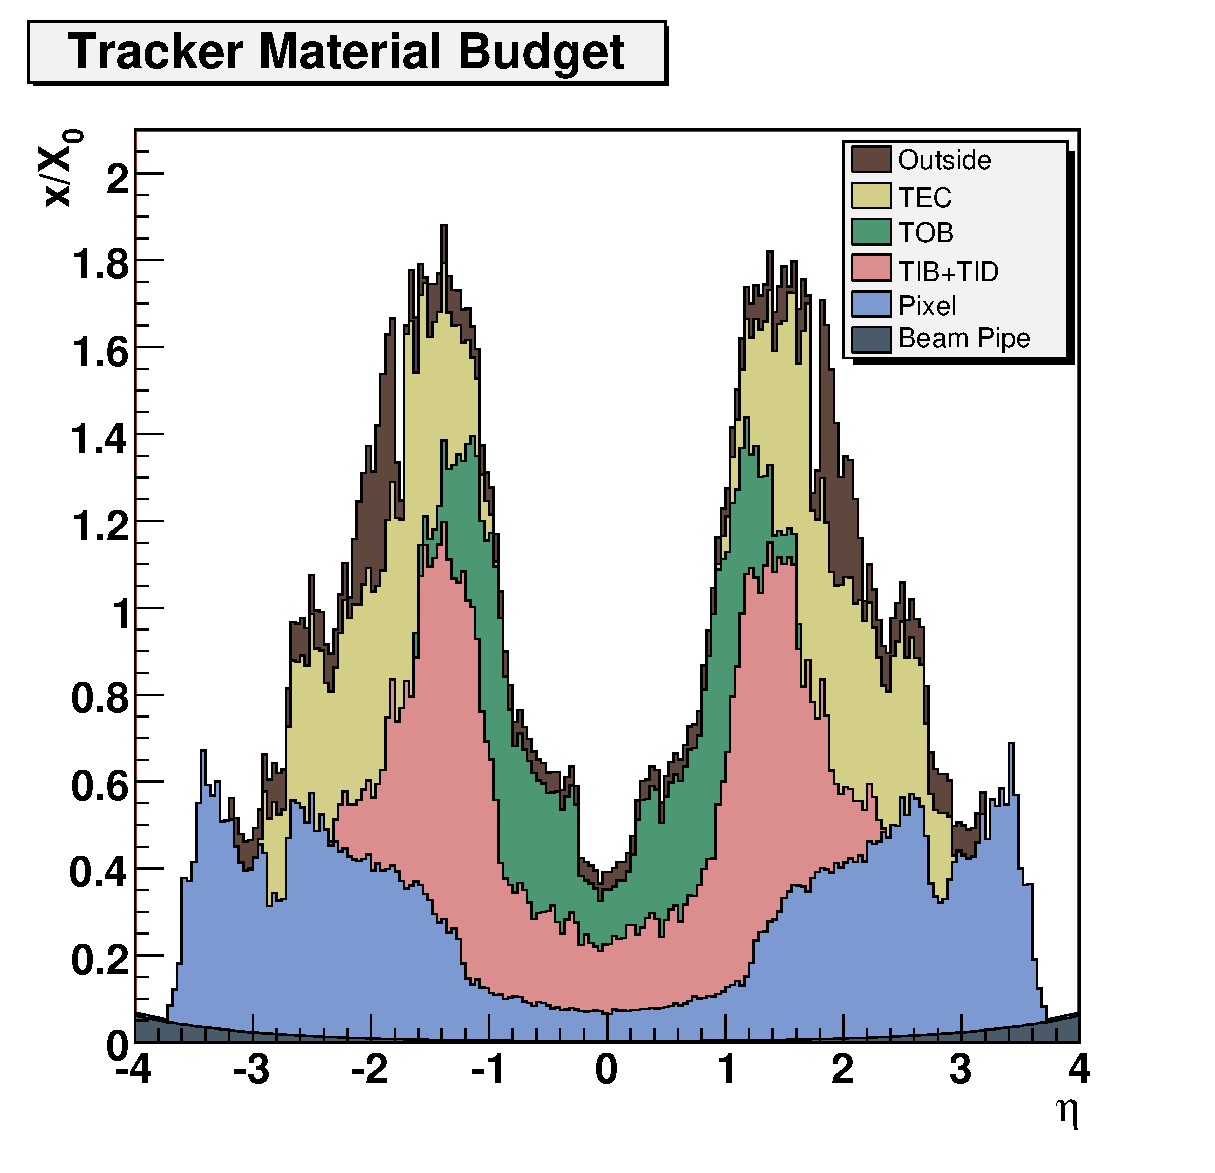
\includegraphics[width=\textwidth]{images/Tracker_SubDetectors_x_vs_eta.eps}
    \end{subfigure}	
  	\caption[Tracker Material Budget]
   	{Tracker material budget, x/$X_{0}$ vs. $\eta$}
	\label{fig:trackerMaterial}
\end{figure}

The material budget of the tracker can be characterized by the rate at which a particle
passing through it loses energy. The radiation length, $X_{0}$, is the 
mean distance over which a high-energy electron loses all but 1/$e$ 
of its energy by bremsstrahlung %citation needed p.291 PDG ------
and $\frac{7}{9}$ of the mean free path for pair production by 
a high-energy photon. Figure \ref{fig:trackerMaterial}
shows the material budget of the CMS tracker in terms of radiation length as a function of $\eta$. 
Due to the location of cabling, electronics and other services, the material budget of the 
tracker is at a minimum of 0.4 $X_{0}$ at $\eta \approx 0$ and increases to approximately 1.8 $X_{0}$
at $|\eta| \approx 1.4$, after which it decreases. 

%Resolution on the order of 10 micro meters http://arxiv.org/pdf/1007.1988.pdf
\subsection{Pixel Detector}%%%check to be sure where you say pixel system vs. pixel detector 
The pixel detector is the inner most detector of the tracking system and,
covering the region from 4 to 15 cm in radius, is the closest detector to 
the interaction point. It has a high granularity and contributes precise 
tracking points in $r-\phi$ and $z$ and is therefore responsible for a small impact 
parameter resolution that is important for b and c-jet secondary
vertex reconstruction and $\tau$-lepton secondary vertex reconstruction.

\begin{figure}[hb]
  \centering
	\includegraphics[width=0.7\textwidth]{images/pixelLayout.png}
  	\caption[Pixel System Layout]
   	{Pixel System Layout}
	\label{fig:pixelLayout}
\end{figure}

The pixel detector is made up of individual pixel cells with a size of 
100 $\times$ 150 $\mu m^{2}$; it has 66 million active elements and covers
a surface area of 1 $m^{2}$. The pixel detector is composed of three barrel 
layers and two endcap disks for which the pseudorapidity range from $-2.5<\eta<2.5$.
The three barrel layers are located at mean radii of 4.3, 7.3, and 10.2 cm. 
The endcap disks extend from 4.8 to 14.4 cm in radii are located at a mean distance
of $z=\pm35.5$ cm and $z=\pm48.5$ cm from the interaction point. 
As can be seen in figure \ref{fig:pixelLayout} this arrangement allows for 3 tracking points over 
almost the full $\eta$-range of the pixel system. Due to 
particles entering the detector at an average angle of $20^{\circ}$ 
charge-sharing between pixels is achieved which improves position resolution.

The pixel system has a zero-suppressed read out scheme with analog pulse
height read-out. This improves the position resolution due to charge sharing,
it helps to separate signal and noise hits as well as to identify large hit 
clusters from overlapping tracks.
A position resolution on the order of 10 $\mu m$ is achieved.

\subsection{Silicon Strip Tracker}
The silicon strip detector is located outside the inner pixel detector, 
It extends from 25 cm to 110 cm in radius and pseudorapidity up to $|\eta|<2.5$. 
This region has a particle flux on 
the order of 100 times less than what is seen by the inner most layers of 
the pixel detector. It is a complementary system to the inner pixel
detector and has a lower granularity. The silicon strip detector 
has 9.3 million active elements over a total surface area of 198 m$^{2}$
and consists of 3 large subsystems. As can be seen in figure \ref{fig:trackerLayout}, 
the Tracker Inner Barrel and Disks (TIB/TID) extend in radius to
55cm and are composed of four barrel layers with three disks at each.
The Tracker Outer Barrel (TOB) consists of six barrel layers and extends to $\pm118$ cm
in z. Extending beyond this in the z-direction, the Tracker EndCaps (TEC+ and TEX- where the plus and minus
indicate the direction in z) are located from 124cm $<|z|<$280 cm. They are composed of 
nine disks which are populated with up to seven rings of radial-strip silicon detectors.
The combined layouts of the pixel detector and silicon strip detector
result in 8 to 14 high precision measurements of track impact points for 
$|\eta|<2.4$.
  \section{Electromagnetic Calorimeter}
Directly outside of the tracking system lies the electromagnetic calorimeter 
(ECAL) of CMS. The driving criteria of the ECAL design is to provide capability
to detect and measure the decay to two photons of the Higgs Boson. The 
ECAL is designed with the objective of a
fast response time, a fine granularity and resistance to the effects of radiation.
Therefore, recently advanced lead tungstate (PbWO$_{4}$) technology was chosen. 
A preshower detector is placed in front of the endcap. Avalanche photodiodes (APDs)
are used as photodetectors in the barrel and vacuum phototriodes (VPTs) in the
endcaps.
The layout of the CMS ECAL is shown in Figure %Include ECAL figure
The barrel part of the ECAL (EB) covers the pseudorapidity range $|\eta|<1.479$
the endcap part covers the rapidity range $1.479<|\eta|<3.0$.
\subsection{Lead Tungstate Crystals}
The ECAL is composed of 75,848 PbWO$_{4}$ crystals: 61,200 mounted in the 
central barrel part, closed by 7,324 crystals in each of the two endcaps. They 
have a high density of 8.28$g/cm^{3}$ and a short radiation length of 0.89cm. 
The Moli$\grave{e}$re radius (radius of a cylinder containing 90\% of the shower's energy deposit) 
is only 2.2cm. These characteristics result in a fine granularity and a compact
calorimeter. Futhermore, the scintillation decay time of these crystals is of the
same order of magnitude as the LHC bunch crossing time whereby 80\% of 
the light is emitted in 25ns. 
\subsection{Energy Resolution}
The energy resolution in the ECAL can be parameterized as in the following equation:
\begin{displaymath}
\left\frac{\sigma}{E}\right^{2}=\left\frac{S}{\sqrt{E}})^{2}\right+\left\frac{N}{E}^{2}\right+C^{2}
\end{displaymath}
where $S$ is the stochastic term, $N$ the noise term, and $C$ the constant term. 
The individual contributions are described in the following paragraphs.


 \section{Hadronic Calorimeter}
The CMS detector is designed to study a wide range of high energy 
physics processes; measurement of hadronic jets and neutrinos or
physics processes which result in missing transverse energy require
a hadronic calorimeter. 
Located outside the Electromagnetic Calorimeter but still within the
superconducting magnet volume is stationed the Hadronic Calorimeter (HCAL).
The Hadronic Calorimeter is a sampling calorimeter: it consists of layered 
sheets of scintillators interleaved with brass absorber plates. Figure %reference figure for HCAL
shows the placement of the of the four regions of the HCAL, the HCAL Barrel (HB),
the HCAL Endcap (HE), the HCAL Forward (HF) and the outer HCAL (HO). 
%The last of these, the outter HCAL, was not active for the 2011/2012 runs. 
The barrel and endcap HCALs, HB and HE, are located within the 
solenoid magnet. The HB extends across $|\eta|<1.3$ and the HE extends from ___


Due to the technical and environmental demands the HF is based on
Cherenkov Radiationg Quartz technology. The forward region has an overall 
higher particle flux and 



 \section{Muon System}
Good muon detection and resolution is of central importance 
to the CMS detector due it's appearance in the final state of many important processes
(for example H$\rightarrow$ZZ$\rightarrow\mu\mu$ and H$\rightarrow\tau\tau$ 
with $\tau\rightarrow\mu\overbar{\nu_{\mu}}\nu_{\tau}$). 
The muon is a relatively easy particle to detect due to its long life time 
and heavy mass they are less affected by radiative losses and the
CMS detector is capable of reconstruction muon momentum and charge over the entire
kinematic range of the LHC. The muon system covers the region in pseudorapidity
$|\eta|<2.4$, consists of about 25,000 m$^{2}$ and is made up of 3
 different types of gaseous particle detectors: drift tube (DT) chambers, 
 cathode strip chambers (CSC) and resistive plate chambers (RPCs).
 Their selection and location are determined by the environmental
 changes with respect to pseudorapidity. %%%% check this
 
\subsection{Drift Tube System}
The barrel region has a low flux of neutrons (which are left over 
from hadronic decays), a uniform 3.8 T magnetic field and a low 
muon rate. Drift tube chambers with standard rectangular drift cells, 
which are more sensitive to  these environmental effects but are %%% Along with RPC'S?? CHECK THIS!!!
relatively cheaper and easier to produce, are used in this region. 
They cover the pseudorapidity $|\eta|<1.2$ and are stationed within 
the iron yoke. The barrel muon detector consists of 4 concentric
cylinders of drift tube chambers around the beam line. The 3 inner
cylinders have 60 DT chambers while the outer has 70 DT chambers,
these combine to a total of approximately 172,000 sensitive wires.

A diagram of a drift cell is shown in figure %%%Drift cell figure


 \section{Trigger}
The LHC delivers proton-proton collisions at the beam crossing 
interval of 25 ns, this corresponds to a crossing frequency of 40 MHz.
Each interaction, or event, requires 0.5 to 1 megabytes of storage space.
%%%%%%%%%fix here
As it is responsible for all data acquisition, %%fix
the trigger system is the most important subsystem of CMS. 

The CMS trigger system is divided into two parts: the Level 1 trigger 
and the High Level Trigger (HLT). 
The Level 1 trigger uses coarsely segmented
data from only the calorimeters and the muon system to make initial
data selections while holding high resolution data in pipelined memories
in front-end electronics. 
The Level 1 trigger must reduce rates by at least a factor of 10$^{6}$, 
resulting in a final output of approximately 30kHz,
before high resolution data is passed to the HLT.
  \subsection{Level 1 Trigger}
  \subsection{Regional Calorimeter Trigger}
  \subsection{High Level Trigger}
\chapter{Event Reconstruction and Monte Carlo Simulations}
After data is collected it undergoes 'Event Reconstruction'.
At this stage %particles
%a series of algorithm to identify and particles and event variables
%reconstruction estimates the trajectory and momentum of the particle
\section{Track and Primary Vertex Reconstruction}
%%%%%%%%%%%%%%%%Track Reconstruction [31] %TRK-11-001
One of the central design motivations to CMS%fix
is a multi-layer tracker with a low occupancy, high granularity
inner silicon pixel detector and a lower granularity silicon strip detector.
%For the Wbb cross section measurement each event is associated
%to a primary vertex, muons are
%and each jet is required to contain a secondary vertex.
%In the search for a MSSM higgs it is association with a primary vertex
%is also required and tracks are used to identify taus, muons, jets, whatelse?
%These characteristics %cause
%complex algorithms to be developed primarily based on Kalman
%Filter algorithms and 
%write an intro
%Track selection involves selection of tracks which are consistent with being produced promptly in the primary interaction region by imposing requirements on the maximum value of significance of the transverse impact parameter relative to the beam spot
\subsection{Track Reconstruction}
\label{sec:TrackReco}
In a technique known as Combined Track Finding (CTF),
the collection of reconstructed tracks is produced via
multiple iterations of the CTF track reconstruction sequence.
The first three iterations are meant to reconstruct successively
lower $p_{T}$ and quality tracks.%%not quite right actually...
%while iterations four through six recover any tracks 
%not found by previous iterations.

After each iteration the CTF track reconstruction sequence, the hits
associated with tracks are removed; this reduces the combinatorial complexity
and simplifies subsequent iterations in a search for more difficult classes of track (for example,
low $p_{t}$ or which are greatly displaced).
The CTF track reconstruction proceeds as follows:
\begin{itemize}
\item First, seeds are generated which provides the initial track candidates.
Charged particles follow helical paths in the magnetic field therefore five parameters (including curvature)
are needed to define a trajectory; to determine these five parameters at least
3 hits or 2 hits in the pixel detector and a constraint on the origin of the track trajectory from the beam
spot is required. Seeds are built in the inner part of the tracker
and track candidates are reconstructed outwards. This is due to a higher finer granularity 
and hence lower occupancy in the center of the pixel detector. Each iteration of CTF
uses independent quality parameters for seeding layers. 
\item Next, track finding is performed based on the Kalman filter method \cite{KalmanFilter}.
Track finding starts by using the seed trajectories to define and then search
for adjacent layers of the detector with a hit. The next step provides the possibility
of adding an invalid hit in the case where the particle failed to produce a hit.
Finally the track finding algorithm updates the trajectories of the tracks. 
%track fitting by means of kalman filter and smoother
\item Track fitting then is used to adjust for the possibility of bias added during the track
finding stage. The trajectory is therefore refitted using a Kalman filter and smoother with
a Runge-Kutta propagator that takes into account both material effect and accomodates
for a inhomogeneous magnetic field.
%track selection sets quality flags and discards tracks that fail certain criteria
\item The final step is track selection where tracks are required to pass a number of quality
based selection criteria. 
The selection criteria puts a requirement on a track's number of layers %fix
with valid hits, the fit-based $\chi^{2}/dof$, and the track's compatibility
with a primary vertex (PV). In addition to these, several requirements are
imposed as a function of track $p_{T}$, $\eta$, and the number of layers
with valid hits. 
\end{itemize}
The tracks and primary vertices found with this algorithm are known as pixel 
tracks and pixel vertices, respectively. The performance of the track reconstruction
offline software is shown in figure \ref{fig:TrackerPerformance}.
\begin{figure}[t]
  \centering
 \begin{subfigure}[b]{.4\textwidth}
	\includegraphics[width=\textwidth]{images/TrackerEffEta.pdf}
  \end{subfigure}
  \begin{subfigure}[b]{.4\textwidth}
	\includegraphics[width=\textwidth]{images/TrackerEffVtx.pdf}
  \end{subfigure}
  	\caption[Tracker Performance]
   	{Tracker efficiency of muons in $Z\rightarrow\mu\mu$ decays. Measured using Tag and Probe as a function of $\eta$ (left) and number of vertices (right)}
	\label{fig:TrackerPerformance}
\end{figure}
\subsection{Primary Vertex Reconstrucion}
Primary vertices (PVs) are reconstruct in order to locate and determine the associated uncertainty of all
proton-proton interaction vertices regardless of whether it is a 'signal' or 'background' vertex.
Primary vertex reconstruction proceeds in three steps.

The first step is to select tracks based on their association with a primary interaction region.
To do this, a number of quality selections are imposed: they are based upon the significance of the
transverse impact parameter ($d_{xy}$), the number of strip and pixel hits that are 
associated with a track and the normalized $\chi^{2}$ from the fit to the
trajectory. In selecting tracks their is no requirement on the $p_{T}$ of the track; 
this is important so that all PVs including ones from minimum bias events will be reconstructed.

The second step is to cluster the selected tracks based on their $z$ coodinate at their
point of closest approach to the beam spot. This is done using a Deterministic Annealing (DA)
algorithm which finds a global minimum given many degrees of freedom.%%ref DA, More on DA?

The third and final step is to take candidate vertices based on DA clustering in $z$ and use
an 'adaptive vertex fitter' %ref
to compute vertex parameters. These parameters include the 3-D position and covariance matrix,
as well as indicators for the success of the fit such as the number of degrees ($n_{dof}$) of freedom for
each vertex and weights of the track used in each vertex. The adaptive vertex fitter
uses a modified definition of $n_{dof}$ where,
\begin{equation}
n_{dof} = -3+2\sum^{nTracks}_{i=1} w_{i},
\end{equation}
Here, $w_{i}$ is the weight of the $i^{th}$ track. This implies that $n_{dof}$ is strongly
correlated with the number of tracks that are compatible with arising from the interaction
region which means that $n_{dof}$ can be also be used to select true proton-proton interactions.
%Vertex reconstruction [33], [34] 

\section{Electron ID and Reconstruction}
\label{sec:electronReco}
%%%This whole section sucks, fix it.
Electrons traversing the tracker pass through 
material equivalent to 0.4-0.8 $X_{0}$ %fix wording
causing electrons to lose a significant amount of 
energy to radiating photons. %more explanation
This causes a spread in $\phi$. %rewrite this
Accurate measurement of electron energy 
at the initial interaction point
requires collection of photons produced via bremstrahlung.
Electron reconstruction is also spread across $\phi$

First, clusters are formed in the ECAL, these clusters are then 
extended in $\phi$ to form super clusters.
Electrons are seeded using either an ECAL driven or a tracker driven approach.
The ECAL driven approach is more efficient for electrons with $E_{T}>4 GeV$;
in this method, super clusters are selected and then matched back to 
tracks in the inner tracker layers. 
For low energy electrons the energy deposit in the calorimeter
is very broad; in this case the tracker driven approach for electron seeding is used.
In the tracker driven approach all reconstructed tracks are considered
and the bremstrahlung hypothesis is tested
by extrapolating a straight line from the track position to the
corresponding ECAL cluster. The process is 
repeated for all layers and a supercluster is defined
by summing all linked electromagnetic cluster deposits. 
Next, trajectories are reconstructed using a dedicated
model of the electron energy loss and fitted using a Gaussian Sum Filter (GSF) algorithm. %%cite GSF
The GSF algorithm is preferred over the typical Kalman Filter algorithm.
This is because bremsstrahlung energy loss, %don't like this phrase either
as described by Bethe and Heitler, 
does not following a Gaussian distribution. 
So, while the Kalman Filter algorithm is optimal in cases where all probability
densities encountered during track the reconstruction procedure are Gaussian
the GSF algorithm distributions are weighted sums of Gaussians and
appropriately describes electron energy loss as described in the Bethe and Heitler model.
The electron trajectory builder constructs all possible trajectories
for a given seed and the best fit is chosen using a $\chi^{2}$ approach.
Finally, a trajectory smoother is applied.

To improve the electron identification in the MSSM analysis a Boosted Decision Tree (BDT) based %Ref BDT
approach is used. The training has been performed in two
bins of $p_{T}$ and three bins of $\eta$ of the electron as shown in Table~\ref{tab:ElectronID-Thresholds}\@.
The BDT has the following $19$ variables as input:

%been trained on data selecting genuine electron candidates from well reconstructed $Z\to ee$ events and
%mis-identified (fake) electron candidates from $Z$+jets events, from which the electrons, which have
%been used to reconstruct the $Z$ boson candidate have been excluded. 

\begin{itemize}
\item
The normalized $\chi^{2}$ of the common track fit, the number of valid hits in the track fit, the normalized
$\chi^{2}$ of the {\it GSFTrack} fit.
\item
The distance in $\eta$ ($\Delta\eta_{SC}({\rm Track}_{vtx})$) and $\phi$ ($\Delta\phi_{SC}({\rm Track}_{vtx})$)
between the reconstructed super cluster in the calorimeter and the track evaluated at the primary vertex
position, the distance in $\eta$ between the super cluster seed and the track evaluated at the calorimeter
surface.
\item
The cluster shape variables $\sigma_{i\eta,i\eta}$ and $\sigma_{i\phi, i\phi}$, where $i\eta$ ($i\phi$)
indicate the integer label of the electromagnetic calorimeter cell in $\eta$ ($\phi$), the cluster shape
variable $f_{e}=1-e1X5/e5X5$, where $e1X5$ ($e5X5$) indicate the energy deposition in an array of $1 \times 5$
($5 \times 5$) cells in the vicinity of the super cluster seed, the cluster shape variable $R9 = e3x3/E_{SC}$,
where $e3x3$ and $E_{SC}$ indicate the energy in an array of $3 \times 3$ cells in the vicinity of the
super cluster seed and the raw energy of the reconstructed super cluster.
\item
The ratio of the hadronic energy over electromagnetic energy of the super cluster ($H/E$), the ratio of
the super cluster energy over the momentum of the associated track evaluated at the selected primary vertex
($E/P$), the variable $1/E_{e}-1/p_{e}$, where $E_{e}$ and $p_{e}$ indicate the reconstructed energy and
momentum of the electron candidate, the ratio of the electron cluster over the momentum of the associated
track and the ratio of the seed cluster over the associated track, where each time the track momentum
has been evaluated at the surface of the calorimeter.
\item
The ratio of the energy that has been reconstructed in the pre-shower detector over the raw energy of
the reconstructed super cluster. The momentum and $\eta$ of the reconstructed electron candidate.
\end{itemize}

An electron is considered as well identified if the BDT discriminator falls above the thresholds shown
in Table~\ref{tab:ElectronID-Thresholds}\@. In addition the electron candidate is required to have a
distance from the selected primary vertex of $d_{z}<0.1$~cm along the $z$ direction of the experiment
 and $d_{0}<0.02 (0.045)$~cm in the plane perpendicular to $z$ in the $e\mu$ ($\mu\tau_{h}$ / $e\tau_{h}$)
decay channel. Further there should be no missing hits in the inner layers of the pixel detector, no
hits before the selected primary vertex and a vertex fit probability of more than $P>10^{-6}$ to minimize the probability that the electron candidate originates from a photon conversion.
%%%%%%%%%%%%%%%%FIX ME

\begin{table}[!ht]
\begin{center}
\begin{tabular}{|l|c|c|c|}
%\cline{2-4}                                                                                                                                                                
\multicolumn{1}{c}{ }      & \multicolumn{3}{c}{\bf BDT Discriminator Value ($>$)}                 \\
\cline{2-4}
\multicolumn{1}{c|}{ }     & $|\eta|<0.8$      & $0.8 \leq |\eta| < 1.479$  & $1.479 \leq |\eta|$  \\
\hline
$\pt\leq 20$ GeV          & $0.925$           & $0.915$                    & $0.965$              \\
$\pt>    20$ GeV          & $0.925$ & $0.975$          & $0.985$    \\
\hline
\end{tabular}
\caption{
  Thresholds for the BDT discriminator to identify electrons. For electrons with $\pt>20$ GeV the values in braces correspond to the Tight ID working point.}
\label{tab:ElectronID-Thresholds}
\end{center}
\end{table}

% Rejection of Electrons from converted photons [39]

%electron ID ---twiki table

%Electron trigger?? maybe
\section{Muon ID and Reconstruction}
Muons at CMS are reconstructed using information from both the 
tracker and the muon detectors. 
%In Wbb high pt muons
%in h to tautau soft muons used.
%Muon reco [40]
\subsection{Standalone Muon Reconstruction}
Standalone $\mu$ reconstruction uses only tracks from the muon system
to reconstruct tracks using a Kalman filter technique which is seeded
by track segments or Level-1 trigger electronics. Tracks are propagated
in iterative steps taking into account the magnetic field, muon energy loss in the material,
multiple scattering and missing hits in the muon system.
Next a suitable $\chi^{2}$ cut is applied to reject bad hits due to showering,
delta rays and pair production. A backward Kalman filter is then applied,
working from outside in and finally the track is extrapolated to the 
beam-spot and a vertex-constrained fit to the track
parameters is performed.
\subsection{Global Muon Reconstruction}
Global muon reconstruction matches standalone tracks to tracks in the tracking
system. 
Tracks are selected which roughly correspond in momentum and position to 
the standalone muon tracks. This is performed in two steps: First,
tracks are selected in a defined $\eta\times\phi$ region which is centered
on the standalone track. Next, spatial and momentum matching is 
used to select the best matching track. Compatibility of the standalone track and tracker tarck with the
primary vertex is also required. Finally a new 'global track' is created combining
tracker and muon hits; at this stage, no new hits are selected, instead, 
the selected hits are refitted as a global track. If more than one candidate
track pair is matched then the candidate with the best $\chi^{2}$ value
is selected. 
For muons with $p_{T}<200\GeV$ the $p_{T}$ measurement is driven
by the fantastic tracker resoluion, for muons with $p_{T}>200\GeV$,
the global-muon fit can improve the momentum resolution compared
to the tracker-only fit.
In muons with a higher $p_{T}$, as might be found
in the boosted topology of $\Wbb$ it is useful to require that muons
are globally reconstructed.
\subsection{Tracker Muon Reconstruction}
In tracker muon reconstruction, all tracks with $p_{T}>0.5$ GeV
and $p>2.5$ GeV are considered as possible muon candidates. 
Track reconstruction is outlined in Section \ref{sec:TrackReco},
after tracks are reconstructed they are extrapolated to the muon
system taking into account effects due to the magnetic field.
If one muon segment matches the extrapolated track then 
it is defined as a tracker muon.  Where matching requires
the the distance in local $x$ between the segment and the extrapolated
track is less than 3 cm or the pull for local x is less than 4 where
the pull is defined as the difference in the position of the matched segment
and the position of the extrapolated track divided by the sum of 
the uncertainties on the position of the matched segment
and the position of the extrapolated track.
%Muon ID (use old muon plots?) mention muon veto in analysis
%Muon trigger

%\section on PF??
% section on lepton isolation?
\section{$\tau$ ID and Reconstruction}
The $\tau$ lepton's high mass means that the $\tau$ plays a very important
roll in search for the SM higgs boson, and MSSM higgs bosons.
The life time of the $\tau$ is short enough that they decay before reaching the inner
most detector. This short lifetime makes $\tau$ reconstruction particularly challenging;
the solution is to reconstruct the decay products of the $\tau$. 

The dominant hadronic $\tau$ decays ($\tau_{h}$) 
and intermediate any intermediate resonances are 
outlined in Table \ref{tab:decay_modes}. 
These decays consist of one or three charged $\pi$ mesons and up to two $\pi^{0}$ mesons.
This thesis uses the hadron plus strips (HPS) algorithm for the reconstruction of 
$\tau_{h}$'s. %%%%ref tau id paper
\begin{table}[b]
\begin{center}
%\tablesize
\begin{tabular}{|l|c|c|c|}
\hline
Decay mode & Resonance & Mass (MeV) &  Branching fraction (\%) \\
\hline
$\tau^{-}$  $\rightarrow $  $h^{-} \nu_{\tau}$ &  &  & $11.6\%$ \\
$\tau^{-}$  $\rightarrow $  $h^{-} \pi^{0}  \nu_{\tau}$ & $\rho^{-}$ & 770 & $26.0\%$ \\
$\tau^{-}$  $\rightarrow $  $h^{-} \pi^{0}\pi^{0}  \nu_{\tau}$ & $a_{\rm{1}}^{-}$ & 1200 & $9.5\%$ \\
$\tau^{-}$  $\rightarrow $  $h^{-} h^{+} h^{-} \nu_{\tau}$ & $a_{\rm{1}}^{-}$  & 1200 & $9.8\%$ \\
$\tau^{-}$  $\rightarrow $  $h^{-} h^{+} h^{-}\pi^{0}  \nu_{\tau}$ & & & $4.8\%$ \\
      \hline
\end{tabular}
\caption{
   Branching fractions of dominant hadronic $\tau$ decays and mass of any intermediate resonance. 
   }
\label{tab:decay_modes}
\end{center}
\end{table}
The HPS algorithm takes into account photon conversions in the CMS tracker
material. %the electron positron decays will bend in the magnetic field
therefore %the HPS algorithm, say something about PF particles
reconstructs photons into 'strips' which are objects which are built%fix
out of electromagnetic particle particles within a window of size $\delta\eta=0.05$
and $\delta\phi=0.20$. The algorithm starts by centering a strip on the
most energetic electromagnetic particle within the PF jet, next it searches
for other electromagnetic particles within the window. If another electromagnetic
particle is found then the object gets associated with the strip and
the four-momentum is recalculated. This procedure is repeated until no other
particles are found. Strips which satisfy the requirement of $p_{T}^{strip}>1GeV/c$
are finally combined with the charged hadrons to reconstruct individual
$\tau_{h}$ decay modes.

The following decay topologies are considered by the HPS $\tau$ ID algorithm:
\begin{itemize}
\item{\bf Single hadron}
      corresponds to $ h^{-} \nu_{\tau}$
      and $ h^{-} \pi^{0} \nu_{\tau}$ decays
      in which the neutral pions have too little energy to be reconstructed as strips.
\item{\bf One hadron $+$ one strip}
      reconstructs the decay mode $ h^{-} \pi^{0} \nu_{\tau}$
      in events in which the photons from $\pi^{0}$ decay
      are close together on the calorimeter surface.
\item{\bf One hadron $+$ two strips}
      corresponds to the decay mode $ h^{-} \pi^{0} \nu_{\tau}$
      in events in which photons from $\pi^{0}$ decays are well separated.
\item{\bf Three hadrons}
      corresponds to the decay mode $ h^{-} h^{+} h^{-} \nu_{\tau}$.
      The three charged hadrons are required                                                                                                      
      to come from the same secondary vertex.
\end {itemize}

Charged hadrons and strips are required to be contained within a cone
of size $\Delta R=(2.8\GeV/p_{T}^{\tau_{h}})$ where $p_{T}^{\tau_{h}}$ is 
the transverse momentum of the $\tau$ hadron $p_{T}^{\tau_{h}}$ is 
required to match the $(\eta,\phi)$ direction of the original PF jet within
a radius of $\Delta R=0.1$. 
%%four momenta must match decay modes
%50-200 MeV for pi0, 0.3 to 1.3 GeV for \rho
%and 0.8 to 1.5 GeV for $a_{1}$

%%%%Tau Isolation from paper
%%%Tau performance plots

\section{Particle Flow Reconstruction}
In proton-proton collisions, even at energies on the order of a few TeV, 
most stable particles produced have a low $p_{T}$.
At CMS, to identify and reconstruct these stable particles a particle flow (PF) event 
reconstruction technique has been developed. PF event reconstruction links 
information %find a better word
about reconstructed tracks and calorimeter deposits
to form object collections of 
electrons, muons, photons, charged and neutral hadrons, HF hadrons and HF EM particles
for each event. These collections can then be used to build taus, Jets, $E_{T}^{miss}$
and to quantify lepton isolation and tag jets originating from heavy quarks.

The first step of PF reconstruction is to perform
iterative tracking. Here, tracks are first seeded and reconstructed with tight criteria
where the emphasis is on achieving a low fake rate. 
After a track has been identified its hits in the tracker are removed and successive iterative steps
then loosen track identification criteria.

The second step of PF reconstruction is to produce clusters in the ECAL and the HCAL. 
In this step cluster seeds are produced from local calorimeter cell energy maxima
then topological clusters are grown by combining cells with at least one common side
with a cell already in a cluster. 

The final step in PF reconstruction, is to apply a link algorithm which links
hits in the ECAL, HCAL, tracker and muon system. The link algorithm
begins with the outer most hit in the tracker and extrapolates
first to the 2 layers of the ECAL pre-shower. Next, it searches for topological clusters
in the ECAL that correspond to a maximal depth expected of a typical
electron energy deposit profile. Then, A search for topological clusters in the
HCAL is performed at a depth corresponding to 1 $X_{0}$.
The track is linked to any given depth if the extrapolated position in 
the calorimeter is within cluster boundaries. The cluster can be enlarged by up 
to once cell to account for discontinuities in the detector elements, radiation via
bremsstrahlung or pair production. Finally, a link between a charged-particle
track in the tracker and a muon track in the muon system is established
when a global fit returns an acceptable $\chi^{2}$ value.

After these links have been established PF reconstruction is performed which
can be summarized into three steps. First, Electrons are created using GSF filter,
this is further described in section \ref{sec:electronReco}. After electrons
are reconstructed their tracks and calorimetric deposits are removed. Next, 
PF charged hadrons are constructed by identifying links between tracks in the 
tracker and clusters in the ECAL. If the energy deposit in the ECAL is 
the same as the total $p_{T}$ in the tracker within calorimetric uncertainty a 
PF charged hadron is created. If the energy in the calorimeters is much higher
than a PF photon or a PF neutral hadron might also be created. If the energy in 
the calorimeters is too small then a relaxed search for hits in the muon system
is performed. Finally, remaining clusters of ECAL and HCAL clusters give rise
to PF photons and PF neutral hadrons. Figure %insert PFjet figure
shows relative fractions of charged hadrons, photons, neutral hadrons, electrons,
hf hadrons and em particles in jets.

\section{Jet ID and Reconstruction}
%Anti-Kt algo [43]
Jet clustering algorithms have become a crucial part of %%finish  this

Jet clustering in this thesis is performed using the anti-$k_{T}$ jet clustering algorithm.
%The primary motive behind choosing the Anti-$k_{T}$ algorithm is that it is 
In order to perform %new word
comparisons with perturbative effects in theoretical calculations jet clustering algorithm
must be both infrared and collinear (IRC) safe. %check/expand
The development and subsequent choice of the anti-$k_{T}$ jet clustering algorithm
was stimulated by questions of sensitivity to non-perturbative effects like hadronization
and underlying event contamination. Previously used jet clustering algorithms
such as the $k_{T}$ %ref
and Cambridge/Aachen %ref
jet clustering algorithms were IRC safe, however, they
had the property that soft radiation could provoke irregularities in the boundaries
of final jets. 
Algorithms such as SIScone %ref
that were soft-resilient were not %%% IRC safe?

To perform jet clustering in the anti-$k_{T}$, $k_{T}$ and Cambridge/Aachen jet algorithm
a distance $d_{ij}$ is introduced between PF particles $i$ and $j$ and $d_{iB}$ between
the entitiy and the beam (B). The clustering proceeds by identifying the smallest distances.
If it is $d_{ij}$ the entities $i$ and $j$ are combined. However if it is $d_{iB}$ then $i$ 
is considered a jet and all its entities are removed from the list of PF particles. The procedure
is repeated until no entities are left. The definition of $d_{ij}$ and $d_{iB}$ are,
\begin{equation}
d_{ij}=\mathrm{min}(k_{ti}^{2p},k_{tj}^{2p})\frac{\Delta^{2}_{ij}}{R^{2}}
\end{equation}
\begin{equation}
d_{iB}=k_{ti}^{2p}
\end{equation}
where $\Delta_{ij}^{2}=(y_{i}-y_{j})^{2}+(\phi_{i}-\phi_{j})^{2}$, $k_{ti}$ is the 
transverse momentum, $y_{i}$ is the rapidity and $\phi_{i}$ is the azimuthal angle of 
the particle $i$. 
$k_{T}$ is %%write this in
The case where $p=1$ is the $k_{T}$ algorithm, $p=0$ corresponds to the Cambridge/Aachen
algorithm and $p=-1$ is the anti-$k_{T}$ algorithm.
The effects of each of these algorithms on an event with a few well-separated hard particles
and many soft particles is shown in figure%%%insert antikt figure.
%Jets used in this analysis use R=0.5
%The key feature is that soft particle do not modify the shape of the jet while hard particles do.

%Jet energy corrections [44]

%Pileup ID
\subsection{b-Jet ID}
%CSV algorithm
%SV in jets
\section{Missing Transverse Energy}
Missing transverse energy is defined using PF candidates as.
\begin{equation}%%%add vectors above everywhere
E_{T}^{miss} = -\sum_{i} p_{T}
\end{equation}
where $i$ runs over all reconstructed PF candidates. 
To improve the $E_{T}^{miss}$ resolution in 
events with jets and neutrinos in the decay products 
which are expected to have a high $E_{T}^{miss}$, such as $\Wbb$,
recoil corrections are applied to the $E_{T}^{miss}$. MVA 
$E_{T}^{miss}$ is used in the search for a MSSM $h\rightarrow\tau\tau$;
MVA $E_{T}^{miss}$ aims at improving further the $E_{T}^{miss}$
through use of recoil corrections and an MVA which targets the true value of the $E_{T}^{miss}$.
These procedures are described in the next sections.
\subsection{Recoil Correction}
Momentum conservation in the transverse plane requires,
\begin{equation}
E_{T}^{miss}+q_{T}+u_{T}=0
\end{equation}
where E_{T}^{miss} is the missing transverse energy,
$q_{T}$ is the vector boson transverse momentum which is measured
in $Z\rightarrow\mu\mu$ events and matched to simulation in $W\rightarrow\mu\nu$.
Finally, u_{T} is the transverse momentum of the hadronic recoil.
\begin{equation}
u_{T}\equiv\sum_{j} p_{j,T},
\end{equation}
where the index $j$ runs over all particles initiating at the interaction point excluding
the vector boson. 

\subsection{MVA $E_{T}^{miss}$}
MVA PF $E_{T}^{miss}$ is based on a set of multivariate regressions.
The purpose of the multivariate regression is to improve measurement of the $E_{T}^{miss}$
in the presence of high pileup.
MVA $E_{T}^{miss}$ is computed as a correction to $u_{T}$. This correction
is performed in two steps: %using two bdts
first, compute a correction to the azimuthal angle
of $u_{T}$ by training a BDT with the true hadronic recoil, $-q_{T}$, as the target. Next
 a separate BDT is trained to predict the magnitude of $u_{T}$. This corrected
 $u_{T}$ is then used in equation %%%cite equation with recoil
 to calculate a new MVA $E_{T}^{miss}$. %list variables? Do I care? it's an f*ing BDT.

%%DESCRIBE LO, NLO, ect
%%DESCRIBE POWHEG
\chapter{Event and Detector Simulation}
Event simulation is crucial
in order to measure detector acceptances and efficiencies 
for various physics processes and to estimate backgrounds 
due to known but SM physics processes. 
Event simulation requires
prediction of a physics process expected at the LHC, production
of physics final states and distribution in phase space of final state particles
and then simulation of particle interactions within the detector\cite{Buckley:2011ms}. %%fix
The physics process is simulated using a monte carlo (MC) generator
while the simulation of the detector is performed using a dedicated
software package which models in interactions of particles
in their passage through matter.  
The output of simulation should be similar if not the same as
the output of the detector; in this way the simulation and data can undergo the
same reconstruction and analysis.
Simulations are initiated using a program called an 'event generator'.
The purpose of an event generator is to produce hypothetical
events with a distribution of observables as predicted by theory.
%simulated in geant4
%They can then be handed to a detector simulator such as Geantfour
%what is an event generator
%need more here
Event simulation can be used for the following:
\begin{itemize}
\item Aid in the design of detectors and experiments.
\item Provide a prediction 
of what physics processes can be expected and at what rates
\item As a tool for devising analysis strategies to optimize signal significance and
reduce unwanted backgrounds.
\item As a framework to in which to test signal significance.
\item As a means to test current physics theory/model and aid in the confirmation of new physics discovery.
\end{itemize}
In the study of particle physics it is important to not 
trust completely a single generator; if particle physics where perfectly
understood and well modeled then there would be no point in building a detector! 
Instead, it is important to understand the ingredients that go into 
a simulation and choose a generator which describes well the desired process. 
A number of physics generators
are in common use; a few of these are outlined in section \ref{sec:MCGenerators}.
Physics simulation can be divided into a few key components:
The hard scattering matrix elements, which define the process(es) under study,
the structure function, which models the momentum distributions of the partons
which are involved in the collision, final and initial state radiation and underlying
event processes including multiple interactions in the detector.
%\section{Physics Event Generation}
\section{Hard Scattering Process}
Hard scattering matrix element generation of a hard scattering process 
begins typically with a well defined subprocess.
Considering the simulation of 
the process $W\rightarrow\mu\nu$ we start with the leading order differential cross section defined as,  
\begin{equation}
d\sigma(\bar{q}q'\rightarrow W^{-}\rightarrow \mu^{-}\bar{\nu_{\mu}})
=f(x,\mu_{F})f'(x',\mu_{F})\frac{1}{2\hat{s}}|\mathcal{M}(\bar{q}q'\rightarrow W^{-}\rightarrow \mu^{-}\bar{\nu_{\mu}})|^{2}
\frac{d\cos\theta d\phi}{8(2\pi)^{2}}
\label{eq:matrixEle}
\end{equation}
%subject to the kinematic constraint that x1x2S=s where S 
%and s are the collider and subprocess centre of-mass energies-squared respectively
where the decay angles $(\theta,\phi)$ of the $W^{-}$ are two degrees of
freedom. $\mathcal{M}$ is the relevant matrix element, 
$q$ and $q'$ are the initial partons,
$1/(2\hat{s})$ is the parton flux and
 $\hat{s}=xx's$ where $s$ is the center of mass energy squared.
The factorization scale is $\mu_{F}$ and has the physical 
interpertation as a collinear cutoff\cite{Maltoni:2007tc}.  
%In typical event generators which simulate hard processes 
%ref equation
Equation (\ref{eq:matrixEle}) is used to write an event generator. 
To do this first a sampling of the relevant phase
space must be performed using a random number generator which selects
momenta of the colliding constituents by sampling
the parton distribution function of the proton at the energy scale
of the subprocess.

Next, the events must be unweighted using the hit-and-miss 
technique to produce events with observables. %%this is terrible, fix later? jan 8th
The relevant phase space for this process is two dimensional: -1 $< \cos\theta <$ 1,
0 $< \phi < $ 2$\pi$. The values of $cos\theta$ and $\phi$ can be chosen using
a uniform random number generator. 
Evaluating the equation (\ref{eq:matrixEle}) at $d\sigma(\theta_{i},\phi_{i})$ gives
that candidate event's differential cross section which is equivalent to the 
probability of this event occurring. The average of many candidate event's differential
cross section, $\langle d\sigma\rangle$, is an approximation to $\int d\sigma$ and converges
to the measured cross section.
So far, the candidate events are distributed flat in phase space and there is 
no physics information in the distributions.
The next step then is to unweight the event using the 'hit-and-miss' technique
so that they are distributed according to theoretical prediction. By unweighting
the events are generated with the frequency predicted by the theory 
being modeled and individual events represent what might be observed in a
trial experiment. 

%Parton Distribution Functions
%Parton Showering and Hadronization
\subsection{Parton Showering, Hadronization and the Underlying Event}
To successfully simulate a process in a hadron hadron collider the simulated event must include 
parton showering, hadronization and simulation of the underlying event.
Parton showering is a form of correction to the hard scattering subprocess
where it is not feasible to calculate these processes exactly.
Programs that use the parton shower approach are also
able to simulate a wide variety of initial and final state processes.

\begin{figure}[hb]
  \centering
	\includegraphics[width=0.5\textwidth]{images/stringModel.png}
  	\caption[Lund String Model for Parton Showering]
   	{Lund String Model for Parton Showering}
	\label{fig:StringModel}
\end{figure}

The Lund String model for parton showering is based on models from lattice QCD simulations
which show that at large distance the potential energy of color sources increases
linearly with their separation. 
A schematic of parton showering using the Lund String model is 
shown in figure \ref{fig:StringModel}. 
Considering the production of a quark-anti-quark pair,
at first the quark and anti-quark are 
moving apart very quickly. A gluonic string is stretched between them. 
Its potential energy grows causing a reduction in the kinetic energy of the
quark-anti-quark system. When the gluon's potential energy reaches
the order of a hadron mass the gluon string breaks apart and a quark-anti-quark
pair is produced.

\begin{figure}[t]
  \centering
	\includegraphics[width=0.75\textwidth]{images/EventProcess.png}
  	\caption[Event Process in a Hadron Collision]
   	{The basic simulation structure for an event in a hadron collision including parton distribution, hard subprocess, parton showering, hadronization, final decay and pileup (Minimum Bias Collisions) \cite{GuidebookOfMcGenerators}.}
	\label{fig:EventProcess}
\end{figure}

For a lepton-lepton collider, the energies of the initial state leptons
is determined by the accelerator and is well known. For a
hadron-hadron collider each hadron is regarded as a collection
of quarks, antiquarks and gluons each of which carries
some fraction $x$ of the hadron's momentum at a scale $Q$ with a 
number density $f(x,Q^{2})$. $Q$ characterizes the hard scattering 
($Q^{2}=M^{2}_{l^{+}l^{-}}, p_{T}^{2}$, ect.)
and changes on the order of $O(1)$ are equivalent\cite{Campbell:2006wx}. 
%In a proton-proton interaction a parton is resolved
%at scale $Q$ and momentum fraction $x$ from each
%proton. 
Figure \ref{fig:EventProcess} 
shows a proton-proton collision where a valence quark
is separated from one of the colliding protons and a 
a sea anti-quark is separated from the other of the colliding protons.
The phenomenology of the parton interaction is encoded
in the parton distribution function $f(x,Q^{2})$. 
The parton distribution function represents the probability
densities to find a parton carrying
a momentum faction $x$ at a squared energy
scale $Q^{2}$\cite{Martin:2009iq}. 
Since the hadronization scale is much smaller than the hard scale the impact
of the hadronization model choice on the final state is typically
small for most physics analyses. 
%Parton showers are essential in providing the %%exclusive?
%description of the event: at leading order the transverse momentum
%for the $W$ will always be zero since there is nothing for the $W$
%to recoil against.

The beam remnants are the colored remains of the proton which
are left behind when the parton which participates in the hard subprocess
is pulled out. As the beam remnants are color connected to the hard
subprocess they should be included in the hadronization system. 
Multiple parton interactions (MPI) where more than one pair
of beam partons interact are also simulated. 
Due to the composite nature of hadrons and the low impact
parameter of spectator partons MPI
have an increase rate of occurrence in the presence of a 
hard scattering process. 
Figure \ref{DPSandSPS} shows a comparison of feynman diagrams for W+jj interaction from 
double parton scattering (an MPI interaction) and single parton scattering. 
In the $\Wbb$ analysis the effects from double parton scattering must be taken into 
account when calculating the measured cross section. 
MPI agreement between data and simulation is tested 
by observing the relative $p_{T}$ balance of the two 
jets via the ratio of $(p_{T,j_{1}}+p_{T,j_{2}})/p_{T,j_{1},j_{2}}$ \cite{Chatrchyan:2013xxa}.

\begin{figure}[hb]
\centering
  \begin{subfigure}[b]{.475\textwidth}
	\includegraphics[trim = 0mm 0mm 0mm 0mm, clip,width=\textwidth]{images/figs_SPS_final.png}
	\end{subfigure}	
   \begin{subfigure}[b]{.475\textwidth}
	\includegraphics[trim = 0mm 0mm 0mm 0mm, clip,width=\textwidth]{images/figs_DPS_final.png}
    \end{subfigure}	
  \caption[]
   	{Single Parton Scattering and Double Parton Scattering in a W+jj event}
    \label{fig:DPSandSPS}
\end{figure}

The LHC is a high luminosity experiment. Therefore, 
an obseved event will have, as background, interactions from other colliding protons.
Successful event simulation must include  
pileup from other proton-proton collisions.
%b quarks are not expected to be
%produced at any signi�cant rate in nonperturbative processes [1], and they do not occur
%as valence �avours of the commonly used beam particles. A priori, they are therefore
%excellent probes of the underlying hard dynamics, whether that involves standard QCD
%processes or various kinds of new physics
\section{Monte Carlo Generator Programs}

\label{sec:MCGenerators}
A number of monte carlo (MC) generators are used to simulate
physics processes. The MC method makes use of a random
number generator to simulate event to event fluctuations
which are intrinsic quantum processes. 
The choice of MC generator is largely dependent on the 
type of process to be simulated. %fix
%K-factors
\subsection{MadGraph}
MadGraph\cite{Alwall:2007st} is is a matrix element generator for SM processes at
any collider. It provides a computation of tree-level matrix elements
with a fixed number of partons in the final state. 
For a user-specified process MadGraph generates
the amplitudes for all relevant subprocesses and produces
the mappings for the integration over the phase space. 
The final state only events may be passed directly to a shower MC program.
\subsection{Tauloa}
Tauloa\cite{TAUOLA} is a package which is used for generation of tau lepton decays including
spin polarization. For each tau decay mode there is a individual phase space generator,
modeling of the weak decay including first order QED corrections for leptonic decays
and a part describing the hadronic current.
\subsection{PYTHIA}
At leading order $\mathtt{PYTHIA}$\cite{Pythia} 
contains approximately 240 different $2\rightarrow n$ subprocesses.
The initial state shower is based on backwards evolution whereby the 
hard scattering process is simulated and is evolved backwards in time to the shower
initiators. Partons radiated in the initial state can initiate final-state showers
of their own. The Lund string model is used in hadronization; it is based on linear confinement
where quarks  are located at the ends of the string and gluons
are energy and momentum carrying kinds in the string. The production of a new $q\bar{q}$
pair causes the string to break. A quark from one break can combine with an antiquark
from an adjacent quark to form a meson. 
\subsection{MCFM}%reread carefully
Monte Carlo for FeMtobarn (MCFM)\cite{MCFM} processes at hadron 
colliders is a parton-level Monte Carlo
program which gives next to leading order predictions for 
a range of processes at hadron colliders. The difference between leading and 
next to leading order is described in section \ref{sec:SMSection}.
 MCFM
produces weighted events and therefore can
give very accurate predictions for event rates at NLO with cuts included, 
however it gives very little information about regions of phase space which are 
dominated by multiple parton interactions. 
Since the final state contains partons rather than hadrons, full detector simulation cannot
be performed using the MCFM output. Furthermore, a parton to hadron correction factor
must be included when comparing (for instance) with \PYTHIA, a generator which does
include hadrons in the final state. The parton to hadron correction factor is estimated
for the $\Wbb$ cross section measurement detailed later in this thesis and is shown to give significant
correction to the overall simulated cross section. 
%ref http://mcfm.fnal.gov/mcfm.pdf
\section{Detector Simulation}
$\mathtt{GEANT4}$\cite{GEANT4} is a toolkit for simulating the passage of
photons, muons, electrons, hadrons and ions through matter at energies from 250 eV to 
several PeV. The simulation package models the 
detector geometry, electric and magnetic fields and a wide range 
of initial to final state physics processes.
Geometry simulation includes a detailed model of the experiment
including layout of the detectors and the location of absorbers (cables, cooling systems, ect.)
Run management for recording details of each run as well as
a number of options for the visualization of the simulation output.
Magnetic field simulation makes use of detailed measurements of 
the magnetic field throughout the CMS detector.
$\mathtt{GEANT4}$ uses decay tables for to properly simulate decay rates 
for particles such as $\pi$, $K$ mesons
and resonant baryons based on data from the Particle Data Group\cite{PhysRevD.86.010001}.
The models used for decay of various physics processes are either
theory or data driven and the toolkit offers a large variety of complementary
and sometimes alternative physics models. 
%need transition sentencce
The probability of a particle surviving a distance $l$ 
\begin{equation}
P(l)=e^{-\eta_{\lambda}}
\end{equation}
where $\eta_{\lambda}$ is an exponential distribution which is independent of 
material and energy; therefore, $\eta_{\lambda}=-\ln(\eta)$ and $\eta$ is
a random number on the interval $(0,1)$. \GEANTfour has been an essential and 
very successful tool in the simulation of detector effects at CMS.
\chapter{Measurement of W plus \bbbar Pair Production}
This document describes a study of W boson production
in association with two b quarks, where W bosons are observed via their decays to muons, and
b quarks are identified as two separated jets.
This production channel provides an important testing ground for 
%perturbative electroweak and 
%QCD calculations as implemented in the 
standard model (SM) predictions. 
Previous
measurements of vector boson production with associated b jets
~\cite{Aaltonen:2009qi,D0:2012qt,Aad:2011kp} have shown varying levels of agreement with theoretical 
calculations.
The precise experimental measurement of the $\Wbb$ cross section will therefore provide important
input to refine theoretical calculations in perturbative QCD, as well as validate associated Monte Carlo techniques.
Understanding the  production of $\Wbb$ events is also crucial as they constitute a major background in the
study of processes with two 
separated and well identified b jets in the final state, one of which is
the search for the standard model Higgs boson (H) decaying to $\bbbar$
when produced in association with a weak vector boson.

The analysis uses a sample of proton-proton collisions 
at a center-of-mass energy of $\sqrt{s}$=7 TeV collected in 2011 with the CMS experiment at the LHC, 
corresponding to an 
integrated luminosity of $5.0\fbinv$.
While the CMS detector is described in detail elsewhere~\cite{CMSExperiment}, the
key components for this analysis are summarized here.
The CMS experiment uses a right-handed coordinate system, with the
origin at the nominal interaction point, the x-axis
pointing to the center of the LHC ring, the y-axis pointing
up (perpendicular to the plane of the LHC ring), and the z-axis
along the counterclockwise-beam direction. The polar angle
$\theta$ is measured from the positive z-axis and the
azimuthal angle $\phi$ is measured in the x-y plane.
The absolute value of the transverse
momentum ($\pt$) is calculated as 
$\pt = \sqrt{p_{\rm{x}}^2 + p_{\rm{y}}^2}$.
%%%
A superconducting solenoid occupies the
central region of the CMS detector, providing an axial magnetic
field of 3.8~T parallel to the beam direction.
The silicon pixel and strip
tracker, the crystal electromagnetic calorimeter, and the brass/scintillator hadron
calorimeter are located within the solenoid. A quartz-fiber
Cherenkov calorimeter extends the coverage to $|\eta| <$ 5.0, where pseudorapidity
is defined as $\eta=-{\rm ln}[\tan{(\theta/2)}]$.
Muons are measured in gas ionization detectors embedded 
in the steel flux return yoke outside the solenoid.
The first level of the CMS trigger system, composed of custom
hardware processors, is designed to select the most interesting events
in less than 3 $\mu$s using information from the calorimeters and muon
detectors. 
The high-level-trigger processor farm decreases the event rate from 100 kHz
delivered by the first level trigger to a few hundred hertz, before data storage.

A number of Monte Carlo (MC) event generators are used to simulate the signal and
backgrounds. 
The  events with W or Z boson production, or with $\ttbar$ production, are generated at leading order (LO) 
with \MADGRAPH 5.1~\cite{Madgraph5}, which is interfaced with \PYTHIA 6.4~\cite{Sjostrand:2006za} (also LO)
for hadronization.
Single top samples are generated at next-to-leading order (NLO) with 
\POWHEG2.0~\cite{Alioli:2008gx,Nason:2004rx,Frixione:2007vw}.
Diboson ($\WW$, $\WZ$, $\ZZ$) and multijet samples are
generated with 
\PYTHIA 6.4~\cite{Sjostrand:2006za}. 
For LO generators, the default set of parton distribution functions
(PDF) used to produce these samples is CTEQ6L~\cite{CTEQ66}, while
MSTWNNLO~\cite{Martin:2009iq} is used for NLO generators.
For all processes, the detector response is simulated using a detailed
description of the CMS detector, based on the \GEANTfour~
package~\cite{GEANT}, and event reconstruction is performed with
the same algorithms as used for data.
The simulated samples include additional interactions per bunch crossing (pileup),
the distribution for which comes from data.
Parton showering is simulated with PYTHIA using the Z2 tune~\cite{Field:2010bc}.

A complete reconstruction of the individual particles emerging from each collision event is obtained 
via a particle-flow (PF) technique~\cite{CMS-PAS-PFT-09-001, CMS-PAS-PFT-10-002}. This 
approach uses the information from all CMS sub-detectors to identify and 
reconstruct individual particles in the collision event, classifying 
them into mutually exclusive categories: charged hadrons, neutral hadrons, photons, electrons, and muons.

Muons are reconstructed~\cite{CMS-PAS-MUO-10-002}
by combining the information of the tracker and the muon spectrometer.
The muon candidates are required to be compatible with the primary vertex of the
event, which is chosen as the vertex with highest $\sum \pt^2$ of its associated tracks.
The muon relative isolation is defined as
\begin{equation*}
I^{\rm{rel}} = \left( \sum_{i}
p_{\text{T, charged}}^i+ \sum_{j}  E_{\text{T, photon}}^j  +\sum_{k}  E_{\text{T, neutral}}^k \right) /\pt^{\mu},
\end{equation*}
with the sums running over all the charged and neutral PF candidates,
excluding the muon candidate itself, 
within a cone around the muon direction
defined by  $\Delta R  < \Delta R_{\rm max} = 0.4$,
where
$\Delta R = \sqrt { (\Delta \eta)^2 + (\Delta \phi)^2 }$, and
$\ET$ stands for the
transverse energy.
%A muon isolation variable, $I^{\rm{rel}}$, is calculated as a 
%sum of the transverse energies  momenta of reconstructed PF particles in a 
%around the direction of the muon, normalized to the muon momentum,
%and excluding the contribution from the lepton candidate itself. 
%The muon is required to be isolated
%from any other detector activity according to the criterion $I^{rel}<0.12$. 

These identified, isolated muons are then combined with the missing transverse 
energy $\vecEtm$ of the event to form a leptonic W candidate. 
The missing transverse energy $\vecEtm$ is defined as
the negative vector sum of the
transverse momenta of all reconstructed particles in the event, with $\MET = |\vecEtm|$,
and is corrected using the procedure 
described in Ref.~\cite{WZCMS:2010}.
The reconstructed transverse mass of the system is built from the transverse momentum of the isolated muon 
and the missing transverse energy of the event, 
\begin{equation*} 
M_\mathrm{T} = \sqrt{2 \pt^{\ell} \MET (1-\cos \Delta \phi)}\ ,
\nonumber
\end{equation*}
where
$\Delta \phi$
is the difference in azimuth between $\vecEtm$ and $\vecPtmu$. In $\Wln$ decays the $M_T$ distribution presents a Jacobian peak 
with an edge at the W mass. Therefore it is a natural topological discriminator against non-W final states which yield a lepton candidate and
missing transverse energy, such as QCD multijet processes, 
in which the events concentrate at low values of the $M_T$ variable. 

Jets are reconstructed from the PF candidates.
The anti-$\mathrm{k_T}$
clustering algorithm~\cite{Cacciari:2008gp} with distance parameter of 0.5
is used, as implemented in the \textsc{fastjet}
package~\cite{fastjet1,fastjet2}. 
%The jet energy is corrected
%for pileup in a manner similar to the correction of the energy inside a lepton
%isolation cone. 
Jets are required to pass identification
criteria that eliminate jets originating or being seeded by
noisy channels in the calorimeter~\cite{Chatrchyan:2009hy}.
In addition to this, jets originating from pileup interactions are
rejected by requiring compatibility of the jets 
with the primary interaction vertex. 
Jet energy corrections are also applied as a function of the jet
$\pt$ and $\eta$~\cite{cmsJEC}.

Secondary vertices (SV) are reconstructed inside each jet.
% using the trimmed kalman vertex 
%finder~\cite{XXX}.
This study makes use of the combined secondary vertex (CSV) b-tagging algorithm~\cite{refCSV};
this algorithm makes use of the
long lifetime and high mass of b hadrons
to provide optimized 
b-quark jet discrimination,
by combining information 
about impact parameter significance, secondary vertex, and 
jet kinematics in a likelihood ratio technique. B-tagged jets are selected by imposing a 
minimum threshold on the CSV discriminator value.
The analysis is based on a CSV
discriminator threshold
which provides an efficiency of approximately 50$\%$  for identifying
jets containing b-flavored hadrons while reducing the misidentification probability for light-quark jets to 0.1$\%$~\cite{BTAGNOTE}
%%%% Note that TOP-12-024 quotes 45% - 0.1% 


\begin{figure}
\centering
\includegraphics[width=0.45\textwidth, trim = 0 4cm 0 0, clip=true ]{Wbb/fig1.pdf}
\includegraphics[width=0.45\textwidth]{Wbb/fig1_jetcsv.pdf}

\caption{(left) The highest-$p_{T}$ jet ($\rm{J_{1}}$) before applying b-tagging.
(right) The CSV b-discriminator 
for $\rm{J_{1}}$.}
\label{figA}
\end{figure}


%The b-tagging working point
%chosen for the analysis is the tight one, in which the efficiency of the selection is approximately 60$\%$, 
%while a suppression
%factor for jets from light quarks is approximately 100~\cite{cmsBTAGPAPER}.

The $\Wbb$ selected events are required to have  
an isolated muon with $I^{\rm{rel}}<0.12$, $\pt>25\GeV$, $|\eta|<2.1$,
exactly two jets with $\pt>25\GeV$ and $|\eta|<2.4$, where 
both selected jets must contain a secondary vertex 
and pass the b-tagging CSV requirement.
To reduce the contribution from $\cPZ$-boson production, the 
event is rejected if there is a second muon, without any requirements 
on the isolation and $\pt$, 
which builds with the isolated muon a dimuon system with 
invariant mass $m_{\mu\mu} > 60\GeV$. 
The $\ttbar$ background is reduced by requiring
that there are no additional isolated electrons or muons with  $p_{T}>20\GeV$ in the event and no
jets with $\pt>25\GeV$ and $2.4<|\eta|<4.5$. To reduce the contribution
from QCD multijet events $\MT > 45\GeV$ is also required.

After all the selection requirements the significant background 
contributions are:
$\ttbar$, single top, W+jets (u,d,c,s,g), $\cPZ$+jets (u,d,c,s,b,g) and QCD multijet. 
Contributions of all these backgrounds 
are computed in 
a simultaneous fit, which provides a final estimate for the signal and background yields.

With the exception of QCD, the shapes of the background distributions are taken from simulation. 
A shape for the QCD contribution is obtained directly from  data  from 
a multijet-enriched control region
defined by all the selection requirements, but
requiring the muon to be non-isolated ($I^{\rm{rel}}>0.2$). The QCD uncertainty in the 
final fit is taken to be $\pm$50\%. This uncertainty is large enough to provide coverage for 
normalization and shape mismodelings of the small QCD contribution in the final sample.
% comes directly from the uncertainty on the
%fit in the QCD background-enriched control region.

The initial yields are taken either from data, in estimates based on the 
control regions, or from simulation, normalized to the NNLO predictions.
The shapes and normalizations of the background distributions
are validated in data with a set of control regions.

The W+$\rm{jets}$ (u,d,c,s,g) process, where the jets are not initiated by b quarks,
is the dominant background before applying the selection requirements on the secondary vertex and
b-tagging. Figure~\ref{figA} (left) shows the $\pt$ of the leading jet at 
this preselected stage. The CSV algorithm working point which provides maximum reduction of 
W+$\rm{jets}$ (u,d,c,s,g) is used. 
The CSV b-tagging discriminant for the leading jet is shown in Figure~\ref{figA} (right). The presence of light and charm jets
in the sample is very small at the higher values of the discriminant.
Furthermore, to increase the purity of the sample %maximally reduce the contribution from the $\Wcc$ process 
a secondary vertex is required to be reconstructed in each of the selected jets.
Figure~\ref{figAbis} shows the mass of the secondary vertex of the leading jet ($\rm{J_{1}}$, right) and the sub-leading jet ($\rm{J_{2}}$, left), for the final selection
in the signal region.
These selection requirements have been validated in the $\ttbar$ and $\cPZ$+jets control regions
described below. 
%in the $\cPZ$+bb and $\ttbar$ control regions. 
%The number of secondary vertices before b-tagging for the signal region region is plotted in Figure~\ref{fig}.

\begin{figure}
\centering
\includegraphics[width=0.47\textwidth]{Wbb/fig1a_J1Mass.pdf}
\includegraphics[width=0.47\textwidth]{Wbb/fig1a_J2Mass.pdf}
\caption{Mass of the secondary vertex for the highest-$p_{T}$ jet ($\rm{J_{1}}$, right) and for the second jet ($\rm{J_{2}}$, left) in the signal region.}
\label{figAbis}
\end{figure}

The events selected for the $\ttbar$ control region pass the selection requirements, with
no restrictions on the number of leptons in the event. 
In addition to the two highest-$\pt$ b-tag jets, the events are required to have at least two extra light jets.
This higher jet multiplicity requirement selects a sample that is dominated by $\ttbar$ events.
Figure~\ref{figB} (right) shows the invariant mass of the 
two highest-$\pt$ additional jets (3rd and 4th highest-$\pt$ in the event, $m_{\rm{J_{3}J_{4}}}$). 
In $\ttbar$ events this distribution reconstructs the mass of the hadronically decaying W boson. 
It is used in the final fit to extract the $\ttbar$ background normalization.
% CHECK: Add info on JES? JER?
The simulation describes the observed distributions well both in 
shape and normalization.
%\begin{figure}
%\centering
%\includegraphics[width=0.45\textwidth,trim = 0 4cm 0 0, clip=true ]{Wbb/fig1.pdf}
%\includegraphics[width=0.45\textwidth,trim = 0 4cm 0 0, clip=true ]{Wbb/fig2.pdf}
%\caption{(left) The $\pt$ of the leading-\pt jet, before applying SV and CSV requirements 
%(right) b-tag jet \pt in the single top control region}
%\label{fig1}
%\end{figure}

The $\cPZ$+jets background estimate is validated in a control region where the standard selection 
is applied except that a second muon is required,  $ 70 < m_{\mu\mu} < 100\GeV$. Agreement
between the observed distributions and simulation is observed in this region.

A single-top-quark control region is defined by selecting events in which the
W boson is accompanied by exactly one b jet
passing the described tagging criteria, and an additional forward jet with $|\eta|>$2.8.
No additional vetoes on extra light jets or leptons are applied.
%The events selected for the single-top control region pass the selection requirements 
%except that events with
%extra jets and leptons are allowed. In addition, events with only one b-tagged jet are 
%selected and at least one
%jet is required to have $|\eta|>$2.8.
%Figure~\ref{fig1}(right) shows the $\pt$ of the b-tag jet in this
%control region. 
The simulation describes the single-top production control region
well and therefore
it is used to estimate the yield and shape of the distributions of kinematic variables in the signal region.

One of the dominant systematic uncertainties comes from the 
relative uncertainty on the b-tagging efficiency ($6\%$ per jet), which together with the uncertainty of the light and charm 
jet mistagging efficiencies are taken from Ref.~\cite{BTAGNOTE}.
The jet and muon energy scales are allowed to vary up and down by one standard deviation and
are added to the fit as a binned shape variation.
The uncertainty associated to the pileup description in Monte Carlo is estimated by shifting the overall mean of 
the number of vertices up or down by 0.6 bunch crossings; it has a negligible effect on the analysis.
To account for the $\MET$ uncertainty the component of $\MET$ that is not clustered in jets is scaled by $\pm10\%$.
Uncertainties on the muon efficiency estimation (triggering, identification, isolation) are estimated to be 1\%.
Background normalization is also taken into account, with an uncertainty assigned to each process
according to previous CMS measurements or to the described control regions. 
The luminosity uncertainty, 2.2\%, 
is taken from Ref.~\cite{CMS-PAS-SMP-12-008}.

\begin{figure}
\centering
\includegraphics[width=0.45\textwidth, trim = 0 4cm 0 0, clip=true ]{Wbb/fig4.pdf}
\includegraphics[width=0.45\textwidth, trim = 0 4cm 0 0, clip=true ]{Wbb/fig3.pdf}
\caption{ 
(left) The $\pt$ distribution of the highest-$\pt$ jet in the signal region, normalized to the result of the binned maximum likelihood fit.
(right) The invariant mass of the two additional light jets in the $\ttbar$ control region, also
normalized to the results of the fit.
}
\label{figB}
\end{figure}

The final yields are extracted via a binned maximum likelihood fit.
To constrain the most prominent backgrounds and reduce the final
systematic uncertainty the fit is performed simultaneously on the $\pt$ of the leading jet ($\rm{J_1}$) 
in the signal region after all selection requirements have been applied,
and on the $m_{\rm{J_3 J_4}}$ distribution obtained from the $\ttbar$ control region.
The  $\rm{J_1}$ $\pt$  is chosen as the final fit variable due to its discrimination power against top-related backgrounds.
Figure~\ref{figB} shows the two fitted distributions, $\pt^{\rm{J_1}}$  in the signal region (left)
and $m_{\rm{J_3 J_4}}$ in the $\ttbar$ control region (right), normalized to the results of the fit.

The statistical and systematic uncertainties are introduced in the form of
nuisance parameters via log-normal distributions around the estimated central values.
The fitted yields for each one of the processes can be found in Table~\ref{tab:fitYields}, 
compared to the Monte Carlo predictions.
To calculate the final uncertainties, first the          
total errors are calculated by taking both
the statistical and systematic errors into
account in the fit. Then the systematic nuisance parameters are removed, the fit is re-run
and the statistical uncertainty is 
obtained. The total systematic error is calculated by subtracting in quadrature 
the statistical uncertainty from the total error.
%I am not sure we need this, I think it is irrelevant...


%\begin{table}[htb]
%\begin{tabular}{|c|c|c|c|c|c|c|c|c|c|}
%\hline
%Process                &\Wbb         &W+light          & \Wcc           &Z+jets        &$t\bar{t}$    &Single Top     & VV             &QCD      & Total  \\
%\hline
%Prediction             & 332        & 1.5             & 21          & 31            &596          &160           &19           &33         & 1194   \\
%                       & $\pm66$    & $\pm 0.2$       &$\pm4$       &$\pm 3$        &$\pm35$      &$\pm 13$      &$\pm 3$      &$\pm 17$   & 78  \\
%\hline
%Fitted                 &300         &1                & 20          &32             &647          &170           &17           &33         & 1220  \\
%Yields                 &-56/+63     & $\pm1$          & $\pm 4$     & $\pm 3$       & $\pm 52$    & $\pm 13$     & $\pm 3$     & $\pm 16$  & -79/+84  \\
%\hline
%\end{tabular}
%\caption{Comparison of the expected (before the fit) and measured (after the fit) yields for each of the processes. The uncertainty on 
%the Monte Carlo prediction takes into account the variation allowed in the background contributions in the fit. The uncertainty in the fitted yields
%corresponds to the full uncertainty after the fit.
%}
%\label{tab:fitYieldsHorizontal}
%\end{table}

\begin{table}[htb]
\begin{center}
\begin{tabular}{c c c }
\hline 
Process  & Prediction  & Fitted Yield \\
\hline 
$\Wbb$         & $332\pm66$     & $300\pm60$ \\
$\Wc$, $\Wcc$  & $21\pm4$       & $20\pm4$ \\
W+usdg         & $1.5\pm0.2$    & $1\pm1$  \\
Z+jets         & $31\pm3$       & $32\pm3$ \\   
$\ttbar$       & $596\pm35$     & $647\pm52$ \\  
Single top     & $160\pm13$     & $170\pm13$ \\
WW, WZ         & $19\pm3$       & $17\pm3$   \\
QCD            & $33\pm17$      & $33\pm16$  \\
\hline
Total          & $1194\pm78$    & $1220\pm82$ \\ 
\hline 
\hline
Observed Events & \multicolumn{2}{c}{$1230\pm35 $} \\
\hline 
\end{tabular}
\caption{Comparison of the expected (before the fit) and measured (after the fit) yields for each of the processes. The uncertainty on
the Monte Carlo prediction takes into account the variation allowed to the nuisance parameters in the fit. The uncertainty in the fitted yields
corresponds to the full uncertainty after the fit.
}
\label{tab:fitYields}
\end{center}
\end{table}

The observed number of events in data after selection in the signal region is $N(S+B)_{data}=1230\pm35 $. 
The number of signal events obtained in the binned maximum likelihood fit is $300\pm60$. 

To show the robustness of the $\Wbb$ fit result a separate study was performed with
two selected b-tagged jets that require each jet to fulfill a looser CSV b-tagging criterion, corresponding 
to an efficiency  of 70\%
for jets containing b-flavored hadrons, while the misidentification probability for light-quark jets is 1$\%$.
%%%% Note that TOP-12-024 quotes 60% - 1% 
With the exception of the modification to the CSV threshold, all other selections for the signal
and control region remain unchanged. The $\Wcc$ contribution is non-negligible with this selection,
therefore, the sum of the invariant mass of the secondary vertex found in each selected jet
is used to distinguish between $\Wbb$ and $\Wcc$. The scalar sum of the transverse momenta of the
muon, the $\vecEtm$ and the jets,
$H_{\rm{T}}$, is used to distinguish W+jets from
top contributions. 
The $\Wbb$ signal is extracted via a two dimensional fit of 
$H_{\rm{T}}$ versus
the sum of the the  secondary vertex masses of the highest- ($\rm{J_1}$) and second-highest-$\pt$ ($\rm{J_2}$) jets. 
An equivalent $\ttbar$ control region to the one described in the
tighter selection, based on the reconstruction of the W mass using two light jets, is also used in this case.
The variables $\rm{J_1}$ SV mass + $\rm{J_2}$ SV mass and $H_{\rm{T}}$ are shown in Fig.~\ref{figC}, with yields 
normalized to the results of the fit.
%The fit yield obtained for the $\Wbb$ signal with this alternate selection is 
%$1.13\pm  0.09\stat ^{+0.18}_{-0.17}\syst \pm 0.18 \theo \pm 0.03\lumi \unit{pb.}$.%$\sigma_{\Wbb}=0.867 \pm 0.07 (stat.) ^{-0.129}_{+0.140} (syst.)$. 
%Background processes predicted by
%Monte Carlo are found to change less than 0.3$\sigma$ with the exception of the $\Wcc$ background 
%whose yield is shifted up by 10\%. 
The cross section value computed with this alternative method 
is found to be consistent
with the primary fit results quoted above.

\begin{figure}
\centering
\includegraphics[width=0.45\textwidth]{Wbb/fig3a.pdf}
\includegraphics[width=0.45\textwidth]{Wbb/fig4a.pdf}
\caption{
The distribution of the sum of the masses of the two secondary vertices ($\rm{J_1}$ SV mass + $\rm{J_2}$ SV mass) (left)  and $H_{\rm{T}}$ of the system (right) in the alternative
medium b-tag selection, 
normalized to the results of the cross-check fit. 
%To further distinguish between $\Wbb$ and $\Wcc$ we introduce the variable '$J_{1}$ SV mass + $J_{2}$ SV mass',
%this is simply the sum of the invariant masses of the secondary vertex found in each selected jet. (left)
%The distribution of $J_{1}$+$J_{2}$ SV mass in the alternate two medium b-Tag selection is shown with yields after the fit;
%the $J_{1}$+$J_{2}$ SV mass variable provides powerful discrimination of $\Wbb$ and $\Wcc$ in this
%selection where there are looser b-tagging requirements. 
%(right) Distribution of $J_{1}$+$J_{2}$ SV mass in the two tight b-Tag selection.
}
\label{figC}
\end{figure}

The $\Wbb$ cross section within the reference fiducial phase space
is determined using the following equation:
\begin{equation*} 
\sigma(pp\rightarrow \Wbb) = \frac{N_{Data}-N_{Bckg}}{\Lint~\epsilon_{sel}},
\nonumber
\end{equation*}
where the efficiency of the selection requirements $\epsilon_{sel} = 10.4 \pm 1.0\%$
is estimated with \MADGRAPH. The associated errors correspond to PDFs and to the factorization/matching scales.

The measured cross section is
%, unfolded to the b-hadron level as described above, for muons with
%$\pt > 25\GeV$ and $|\eta|<2.1$ and two b-jets with
%$\pt > 25\GeV$ and $|\eta|<2.4$ is found to be 
%$1.17\pm  0.11\stat ^{+0.21}_{-0.17}\syst \pm 0.18 \theo \pm 0.03\lumi \unit{pb.}$
\begin{eqnarray*}
\sigma(pp\rightarrow \mathrm{W} + \bbbar, p_T^{\mathrm{b}}>25~\GeV, |\eta^{\mathrm{b}}|<2.4)\times{\cal{B}}(\Wmn, p_T^{\mu}>25~\GeV, |\eta^\mu|<2.1) = \\
            =0.53\pm  0.05\stat \pm 0.09 \syst \pm 0.06 \theo \pm 0.01\lumi \unit{pb.} %(FIXME!!! where do we quote the errors of Q2?).
\end{eqnarray*}

%The \MADGRAPH  cross sectioni (FIXME!!! where do we quote the errors of Q2?),
%corrected to the NNLO using the standard reference
%cross-section value in CMS (FEWZ, MSTWNNLO), is
%estimated to be $1.30\pm0.09$ pb (no vetoes) or $0.58\pm0.08 $ pb  (vetoes). 
This cross section is calculated at the level of final-state particles, by requiring a muon with $p_T>25$~\GeV and $|\eta|<2.1$ and
exactly two jets, reconstructed using the anti-$k_T$ jet algorithm with distance parameter 0.5, with $p_T>25$~\GeV and $|\eta|<2.4$ and
each containing at least one b hadron with $p_T>5$~\GeV. Events with extra jets are vetoed.
A hadronization correction factor $0.92\pm0.01$ to extrapolate from the final-state particle jets 
%b-hadron measurement 
to the parton-level cross section 
is estimated with \MADGRAPH+\PYTHIA. At the parton level the events are required to have a 
muon with
$\pt > 25\GeV$ and $|\eta|<2.1$ and exactly two parton-jets with
$\pt > 25\GeV$ and $|\eta|<2.4$ each containing a b parton just before hadronization. This factor has been computed in the 4-flavor and 5-flavor
schemes, and the difference between said calculations is assigned as systematic uncertainty to the measurement.
The simulated partons include double parton scattering and multiple parton interaction 
production of $\bbbar$ pairs, which have been found to reproduce adequately these 
processes observed by CMS measurements. 

The measured values can be compared to the NLO cross section of
%\begin{displaymath}
%$0.94 ^{+0.20}_{-0.15}\unit{pb}$
$0.52 \pm 0.03\unit{pb}$ 
%\end{displaymath}
calculated with MCFM~\cite{Campbell:2010ff, Badger:2010mg}.
The MCFM cross section is calculated using the MSTW2008NNLO~\cite{Martin:2009iq} PDF, and 
setting the normalization and renormalization scales to $\mu_{\rm{F}} = \mu_{\rm{R}} = m_{\PW} + 2m_{\rm{b}}$.
The theoretical cross section uncertainties
are estimated by varying the $\mu_{\rm{F,R}}$ simultaneously up and down by a factor of two, and also take
into account PDF uncertainties computed using standard procedures.

%Correction factors to go from this fiducial measurement to the full phase-space can be computed with MCFM.
%The acceptance correction to extrapolate the measurement in $p_T^{\mu}>25~\GeV$ and $|\eta^{\mu}|<2.1$ to
%the full muon phase-space is found to be ${\cal{A}}(\mu)=0.50\pm XX \textrm{PDF}$. The acceptance correction 
%to remove the veto on extra jets is found to be ${\cal{A}}(\textrm{jet~veto})=0.50\pm XX \textrm{$\mu_{\rm{F,R}}$}$.

\begin{figure}
\centering
\includegraphics[width=0.45\textwidth]{Wbb/fig5.pdf}
\includegraphics[width=0.45\textwidth]{Wbb/fig6.pdf}
\caption{(left) The $\Delta R$ between the two selected b jets
(right) the $\MT$ distribution, normalized to the results of the fit.}
\label{figD}
\end{figure}

In addition to this measurement of the cross section, we have explored the kinematics of the $\Wbb$ system.
The angular distance between two selected b jets, $\Delta R(\rm{J_1,J_2})$ 
and the $\MT$ distribution are compared to Monte Carlo predictions 
in Fig.~\ref{figD}. The shapes are taken from simulation and are normalized to the fit results. 
Figure~\ref{figE} shows the invariant mass of the two 
selected b jets system and its $\pt$.
The observed distributions  are well described by the simulation.
%Those distributions are very important for the dominant background background estimation
%in the $WH\rightarrow l \nu b \bar{b}$ search.


%The measured cross section, unfolded to the b-hadron level as described above, for muons with
%$\pt > 25\GeV$ and $|\eta|<2.1$ and two b-jets with
%$\pt > 25\GeV$ and $|\eta|<2.4$ is found to be 
%$1.17\pm  0.10\stat ^{+0.21}_{-0.17}\syst \pm 0.09 \theo \pm 0.03\lumi \unit{pb.}$

% No quoting MCFM until we fix the C(parton, hadron) factor

In summary, we have presented a measurement of the $\Wbb$ production
cross section in proton-proton collisions at 7\TeV. The $\PW+\bbbar$ events
have been  selected in the $\PW \to \mu\nu$ decay mode with a 
muon of $\pt>25\GeV$ and $|\eta|<2.1$, and two b jets with $\pt>25\GeV$ and $|\eta|<2.4$. 
The data sample corresponds to an integrated luminosity of $5.0\fbinv$.
%The measured cross section
%$\sigma ( \Wbb) =  0.98 \pm 0.12 \stat \pm0.20 \syst \pm 0.07 \theo \pm 0.02\lumi \unit{pb}$
%is consistent with the SM prediction.
The measured cross section 
%$\sigma ( \Wbb) =  0.98 \pm 0.12 \stat \pm0.20 \syst \pm 0.07 \theo \pm 0.02\lumi \unit{pb}$
%$\sigma ( \Wbb) = 1.17\pm  0.10\stat ^{+0.21}_{-0.17}\syst \pm 0.18 \theo \pm 0.03\lumi \unit{pb.}$
$\sigma(pp\rightarrow \mathrm{W} + \bbbar, p_T^{\mathrm{b}}>25~\GeV, |\eta^{\mathrm{b}}|<2.4)\times {\cal{B}}(\Wmn, p_T^{\mu}>25~\GeV, |\eta^{\mu}|<2.1) =0.53\pm  0.05\stat \pm 0.09 \syst \pm 0.06 \theo \pm 0.01\lumi \unit{pb}$
for production of a W boson in association with two b jets is in agreement with
the SM predictions.
This result is approaching the precision of theoretical predictions at NNLO, 
allowing a sensitive test of perturbative calculations
in the SM.


\begin{figure}
\centering
\includegraphics[width=0.45\textwidth, trim = 0 4cm 0 0, clip=true ]{Wbb/fig7.pdf}
\includegraphics[width=0.45\textwidth, trim = 0 5cm 0 0, clip=true ]{Wbb/fig8.pdf}
\caption{(left) The invariant mass, $m_{\rm{J_{1} J_{2}}}$ of the two selected b jets and 
(right) the $p_{T}(J_{1} J_{2})$ distribution, normalized to the results of the fit.}
\label{figE}
\end{figure}

\section{Introduction}
Experimental evidence from a large number of high energy experiments has shown an 
overwhelming success of the Standard Model (SM) of fundamental interactions, although 
some questions remain unanswered like the origin of mass of elementary particles. In 
the SM~\cite{SM1,SM2,SM3}, this is achieved via the Higgs 
mechanism~\cite{Englert:1964et,Higgs:1964ia,Higgs:1964pj,Guralnik:1964eu,Higgs:1966ev,Kibble:1967sv}, 
which also predicts the existence of a scalar Higgs boson. However, the SM Higgs boson 
suffers from quadratically divergent self-energy corrections at high energy. Numerous 
extensions to the SM have been proposed to address these divergences. In the model of 
supersymmetry (SUSY)~\cite{Golfand:1971iw,Wess:1974tw} , a symmetry between fundamental 
bosons and fermions, a cancellation of these divergences occurs. The Higgs sector of the 
minimal supersymmetric standard model (MSSM)~\cite{fayet1,fayet2} has two scalar doublets 
which results in five physical Higgs bosons: a light and heavy CP-even $h$ and $H$, the 
CP-odd $A$ and the charged Higgs boson $H^{\pm}$. At lowest order the Higgs sector can 
be expressed in terms of two parameters which are usually chosen as tan$\beta$, the 
ratio of the two vacuum expectation values, and the mass of the CP-odd boson, $M_A$. 

The dominant neutral MSSM Higgs boson production mechanism is the gluon-fusion process, 
$\Pg\Pg \to h, H, A$, for small and moderate values of tan$\beta$. At large values of tan$\beta$ 
the b-associated production is the dominant contribution, due to the enhanced bottom Yukawa 
coupling. In the region of large tan$\beta$ the branching ratio to tau leptons is enhanced, 
making the search for neutral MSSM Higgs bosons in the di-$\Pgt$ final state of particular interest. 

This Summary reports a search for neutral MSSM Higgs bosons in pp collisions at $\sqrt{s}=$ 7~TeV 
and 8 TeV at the LHC. The data were recorded by the Compact Muon Solenoid experiment (CMS)~\cite{CMS-JINST} 
in 2011 and 2012 and correspond to an integrated luminosity of 24.6 fb$^{-1}$, with 4.9~fb$^{-1}$ 
at 7 TeV and 19.7~fb$^{-1}$ at 8 TeV. Five different $\Pgt\Pgt$ final states are studied: 
$\Pe\Pgt_{h}, \Pgm\Pgt_{h}, \Pe\Pgm$, $\Pgm\Pgm$ and $\Pgt_{h}\Pgt_{h}$, where $\Pgt_{h}$ denotes a 
hadronic decay of a $\tau$. These results are an extension of a previous search by the CMS 
experiment~\cite{CMS-PAPER-HIG-10-002} and are similar to those performed by the the ATLAS 
experiment~\cite{Atlas-MSSM}, the Tevatron~\cite{Tevatron-MSSM, D0-MSSM, CDF-MSSM}, and are 
complimentary to the MSSM Higgs search at LEP~\cite{LEP2-MSSM}. 

Traditionally, searches for MSSM Higgs bosons are expressed in terms of benchmark scenarios where 
the lowest-order parameters tan$\beta$ and $M_A$ are varied, while fixing the other parameters that 
enter through radiative corrections to certain benchmark values. 
In this study, the $m_{h}^{\rm max}$ scenario~\cite{MHMAX-Carena,MHMAX-Carena-2002} is used as it 
yields conservative expected limits in the tan$\beta$ and $M_A$ plane. 
%In this scenario, the parameters are set to the following values: 
$M_{\rm SUSY}$ = 1~TeV; $X_t$ =2$M_{\rm SUSY}$; $\Pgm$ =~200~$\GeV$; $M_{\tilde{g}}$ = 800~$\GeV$; 
$M_2$ = 200~$\GeV$; and $A_b = A_t$, where $M_{\rm SUSY}$ is the common soft-SUSY-breaking squark 
mass of the third generation; $X_t = A_t - \Pgm/\tan\beta$ is the stop mixing parameter; $A_t$ 
and $A_b$ are the stop and sbottom trilinear couplings, respectively; $\Pgm$ the Higgsino mass 
parameter; $M_{\tilde{g}}$ the gluino mass; and $M_2$ is the SU(2)-gaugino mass parameter. 
%The value of $M_1$ is fixed via the unification relation $M_1 =(5/3)M_2\sin\theta_{\rm W}/\cos\theta_{\rm W}$.

Recently the CMS and ATLAS experiments have reported the observation of a new boson with mass 
in the range 125-126~GeV~\cite{CMS-HIGGS-DISCOVERY,ATLAS-HIGGS-DISCOVERY}. 
An indication that this new boson decays into tau pairs has recently been reported by 
CMS~\cite{CMS-PAPER-HIG-13-004}.
If the new boson is interpreted as the light scalar MSSM Higgs $h$, part of the tan$\beta$ a
nd $M_A$ parameter space in the $m_{h}^{\rm max}$ scenario is excluded. 
However, changes in the stop mixing parameter open up a large region of the allowed parameter 
space~\cite{Heinemeyer:2011aa,Carena:2013qia}. 

In this report, the results are interpreted both in the context of the MSSM $m_{h}^{\rm max}$ scenario and also in a model independent way, 
in terms of upper limits on $\sigma\cdot$BR($\Phi\to\Pgt\Pgt$) for gluon-fusion and b-associated neutral Higgs boson production,
where we denote by $\Phi$ any of the three neutral MSSM Higgs bosons.
%In this report, the result is interpreted in the context of the MSSM $m_{h}^{\rm max}$ scenario.




 

\section{Trigger and Event Selection}

%The analysis makes use of the four independent tau-pair final states, $\Pe\Pgt_h$+X, $\Pgm\Pgt_h$+X, $\Pe\Pgm$+X, and $\Pgm\Pgm$+X.
%In all four channels, the reducible and irreducible backgrounds are substantial.

The trigger selection requires a combination of electron, muon and tau trigger objects~\cite{CMS-PAS-EGM-10-004,CMS-PAS-MUO-10-002,CMS-EWK-TAU}. The identification criteria and transverse momentum thresholds of these objects were progressively tightened as the LHC instantaneous luminosity increased over the data-taking period.

A particle-flow algorithm~\cite{CMS-PAS-PFT-09-001,CMS-PAS-PFT-10-002,CMS-PAS-PFT-10-003} is used to combine information from all CMS subdetectors to identify and reconstruct individual particles in the event, namely muons, electrons, photons, and charged and neutral hadrons. From the resulting particle list jets, hadronically decaying taus, and missing transverse energy ($\MET$), defined as the magnitude of the vector sum of the transverse momenta, are reconstructed. 
The jets are reconstructed using the anti-$k_T$ jet algorithm~\cite{Cacciari:fastjet1,Cacciari:fastjet2} with a distance parameter of $R=0.5$. Hadronically-decaying taus are reconstructed using the hadron plus strips (HPS) algorithm, which considers candidates with one charged pion and up to two neutral pions or three charged pions~\cite{CMS-PAS-TAU-11-001}. To tag jets coming from b-quark decays the Combined Secondary Vertex (CSV) algorithm is used. This algorithm is based on the reconstruction of secondary vertices, together with track-based lifetime information~\cite{BTV-11-004}. 

Events in the $\Pe\Pgt_h$ ($\Pgm\Pgt_h$) final state are required to contain
an electron of $\pt >$~20~$\GeV$ (muon $\pt >17~\GeV$) and $|\eta| < 2.1$ plus an oppositely charged $\Pgt_h$ of $\pt > 20~\GeV$ and $|\eta| < 2.3$.
The $\pt$ thresholds for electrons (muons) are increased to $24~\GeV$ ($20~\GeV$) in the 2012 dataset,
following the raise in trigger thresholds at higher instantaneous luminosity.
%In the $\Pe\Pgt_h$ and $\Pgm\Pgt_h$ final states, events are selected in the 2011 (2012) dataset with an electron of $\pt >$~20~$\GeV$ (24~$\GeV$) or a muon of $\pt >17~$\GeV$$ (20~$\GeV$) and $|\eta| < 2.1$ and an oppositely charged $\Pgt_h$ of $\pt > 20~$\GeV$$ and $|\eta| < 2.3$. 
To reduce the contamination of $\cPZ\to\Pe\Pe, \Pgm\Pgm$ background, events with two electrons or muons of $\pt >15~\GeV$, opposite charge and passing loose isolation criteria are rejected.
$\cPZ\to\Pe\Pe$ background in the $\Pe\Pgt_h$ final state is further suppressed by requiring $\MET > 25~\GeV$.
%To reduce the contamination of $\cPZ\to\Pe\Pe, \Pgm\Pgm$ background, events 
%with more than one electron or muon of $\pt >15~$\GeV$$ are rejected and in addition, $\MET$ is required to be larger that 25~$\GeV$ in the $\Pe\Pgt_h$ final state. 
In the $\Pe\Pgm$ and $\Pgm\Pgm$ final states events with two oppositely charged leptons are selected, where the highest-$\pt$ lepton is required to have $\pt >$ 20~$\GeV$ and the second-highest-$\pt$ lepton $\pt >10~\GeV$. Muons with $|\eta|<2.1$ and electrons
 with  $|\eta|<2.3$ are used. 
The large background arising from $\cPZ\to \Pgm\Pgm$ events in the $\Pgm\Pgm$ channel
is removed by a multivariate {\it Boosted Decision Tree} (BDT) discriminator.
In the $\Pgt_h\Pgt_h$ final states events with two oppositely charged hadronic taus with $\pt > 45~\GeV$ and $|\eta| < 2.1$ are selected.
%, where the highest-$\pt$ lepton is required to be more isolated than the second highest-$\pt$ one. 

An average of 10 (20) proton-proton interactions occurred per LHC bunch crossing in 2011 (2012), making the reconstruction of physics objects challenging. For each reconstructed collision vertex the sum of the $\pt^2$ of all tracks associated to the vertex is computed and the one with the largest value is taken as the primary collision vertex. In order to mitigate the effects of pile--up on the reconstruction of $\MET$, a multivariate regression correction is used where the inputs are separated in those components coming from the primary vertex and those which are not~\cite{CMS-PAS-JME-12-002}. 
The correction improves the $\MET$ resolution in $\cPZ\rightarrow\Pgm\Pgm$ events by roughly a factor of two in case 25 additional pile-up events are present. 

Taus from Higgs boson decays are expected to be isolated in the detector, while leptons from 
heavy-flavor (c and b) decays and decays in flight are expected to be found inside jets. A 
measure of isolation is used to discriminate the signal from the QCD multijet background, 
based on the charged hadrons, photons, and neutral hadrons falling within a cone around the 
lepton momentum direction.
A correction is applied to the isolation to reduce the effects of pile-up. For charged particles, 
only those associated with the primary vertex are considered and for neutral particles, a 
correction is applied by subtracting the energy deposited in the isolation cone by charged 
particles not associated with the primary vertex, multiplied by a factor of 0.5 which 
approximately corresponds to the ratio of neutral to charged hadron production in the 
hadronization process of pile-up interactions. An $\eta$, $\pt$, and lepton-flavor dependent 
threshold on the isolation variable of less than roughly 10\% of the candidate $\pt$ is applied.

To correct for the contribution to the jet energy due to pile-up, a median energy density ($\rho$) is determined event by event. The pile-up contribution to the jet energy is estimated as the product of $\rho$ and the area of the jet and subsequently subtracted from the jet transverse energy~\cite{Cacciari:subtraction}. In the fiducial region for jets of $|\eta| < 4.7$, jet energy corrections are also applied as a function of the jet \ET and $\eta$~\cite{cmsJEC}.

%For taus decaying hadronically, the isolation variable is calculated using a multivariate {\it Boosted Decision Tree} (BDT) technique based on the neighboring reconstructed particles. Rings of radius $\Delta R$ = $\sqrt{\Delta\phi^{2} + \Delta\eta^{2}}$ are formed in the vicinity of the identified $\tau_{h}$ candidate and the moments of the energy deposits in $\eta$ and $\phi$ and the energy density $\rho$ in the event is used to define the isolation variables.

In order to reject events coming from $\PW$+jets background a dedicated selection is applied. 
In the $\Pe\Pgt_h$ and $\Pgm\Pgt_h$ final states, the transverse mass of the electron 
or muon and the $\MET$, $M_{T} = \sqrt{2 \pt \MET (1-\cos\Delta\phi)}$, is required to 
be less than 30~$\GeV$, where $\pt$ is the lepton transverse momentum and $\Delta\phi$ is the difference in $\phi$ of the lepton and $\MET$ vector. In the $\Pe\Pgm$  final states, a discriminator is formed by considering the bisector of the directions of the visible tau decay products transverse to the beam direction, denoted as the $\zeta$ axis.  From the projections of the visible decay product momenta and the $\MET$ vector onto the $\zeta$ axis, two values are calculated: $ P_{\zeta} = \left( p_\mathrm{T,1} + p_\mathrm{T,2} + \MET \right) \cdot \zeta\;\;$; $\;\;P_{\zeta}^{\text{vis}} = \left( p_\mathrm{T,1} + p_\mathrm{T,2} \right) \cdot \zeta\;\;$, 
where $p_\mathrm{T, 1}$ and $p_\mathrm{T, 2}$ indicate the transverse momentum
of two reconstructed leptons.  $\Pe\Pgm$ events are selected with $P_\zeta - 1.85 \cdot P_\zeta^{\mathrm{vis}} > -20 $~$\GeV$.



To further enhance the sensitivity of the search for Higgs bosons, the sample of selected events is split into
two mutually exclusive categories:
\begin{itemize}
\item {\bf B-Tag:} This event category is intended to exploit the production of Higgs bosons in association with $b$-quarks 
which is enhanced in the MSSM. At least one $b$-tagged jet with $\pt>20$~$\GeV$ is required  and not more than one jet with $\pt>30$~$\GeV$. 
\item {\bf No-B-Tag:} This event category is mainly sensitive to the gluon-fusion Higgs production mechanism. Events are required to have no b-tagged jets with $\pt>20$~$\GeV$. 
\end{itemize}

%All categories are split in two regions of reconstructed transverse momentum. For the $\Pe\Pgt_h$ and $\Pgm\Pgt_h$% final states the $\pt$ threshold on the hadronic tau is 40~$\GeV$. For $\Pe\Pgm$ final state the threshold on the muon is 35~$\GeV$ and for the $\Pgm\Pgm$ the threshold of the leading muon is 30~$\GeV$.

The observed number of events for each category, as well as the expected number of events from various background processes, 
are shown in Tables~\ref{table:events_mutau}--~\ref{table:events_mumu} together with expected signal yields and efficiencies.

The largest source of background events comes from $\cPZ\to\Pgt\Pgt$, which is estimated using a sample of $\cPZ\to\Pgm\Pgm$ events where the reconstructed muons are replaced by the reconstructed particles from simulated tau decays. The normalization for this process is determined from the measurement of the $\cPZ\to\Pgm\Pgm$ yield in data. 
Another significant source of background is QCD multijet events.
QCD events may contribute to the $\Pgt_h\Pgt_h$ ($\Pe\Pgt_h$ and $\Pgm\Pgt_h$) channel
in case two jets are misidentified as hadronic tau decays (one jet is misidentified as an isolated electron or muon, and a second jet as $\Pgt_h$).
The QCD background contribution in the $\Pgt_h\Pgt_h$ channel
is estimated by measuring, in a control region, the probability for jets to pass hadronic tau identification criteria
and applying these probabilities as weights to events which pass all event selection criteria except tau identification requirements.
In the $\Pe\Pgt_h$ and $\Pgm\Pgt_h$ channels the rate of QCD background is estimated using the number of observed same-charge
tau pair events.
Events from $\PW$+jets in which there is a jet misidentified as a $\Pgt_h$ are another sizeable source of background in the $\Pe\Pgt_h$ and $\Pgm\Pgt_h$ channels.
The rate of this background is estimated using a control region of events with large transverse mass.
Other background processes include $\cPqt\cPaqt$ production
and $\cPZ\to \Pe\Pe/\Pgm\Pgm$ events, particularly in the $\Pe\Pgt_h$ channel, 
as the the probability for electrons to be misidentified as $\Pgt_h$ amounts to 1--2\%.
In the $\Pe\Pgm$ final state, the $\PW +$jets and multijet background events are obtained by measuring the number of events with one good lepton and a second one which passes relaxed selection criteria, but fails the nominal lepton selection.
This sample is extrapolated to the signal region using the efficiencies
for such loose lepton candidates to pass the nominal lepton selection. These efficiencies
are measured in data using observed multijet events. The shape of the \ttbar  and di-boson backgrounds are estimated from simulation 
using \MADGRAPH~\cite{Alwall:2007st} and \PYTHIA~\cite{Pythia}, respectively. The event yields are determined from measurements in background-enriched regions.

The event generator \PYTHIA is used to model the MSSM Higgs boson signal.
Taus are decayed by the \TAUOLA~\cite{TAUOLA} package.
In all Monte Carlo  samples, additional interactions are simulated and reweighted to the observed pile-up distribution.  
The missing transverse energy in Monte Carlo simulated events is corrected for the difference between data and simulation 
measured using a sample of $Z\rightarrow\mu\mu$ events~\cite{CMS-EWK-WZ}.


\begin{table*}[!h]
  \begin{center}
    \caption{Number of expected events in the two event categories in the $\Pgm\Pgt_{\rm h}$ channel, where the combined statistical and systematic uncertainty is shown. 
      The signal yields for the sum of all three neutral MSSM Higgs bosons, A+H+h, expected for $M_{A}$= 160 GeV and $\tan\beta$= 8 are given for comparison.
      Also given are the products of signal efficiency times acceptance for $M_{\Phi}$= 160 GeV.}
\begin{tabular}{|l|r@{$ \,\,\pm\,\, $}l|r@{$ \,\,\pm\,\, $}l|} 
\hline 
Process & \multicolumn{2}{c|}{\emph{B-Tag}} & \multicolumn{2}{c|}{\emph{No-B-Tag}}\\ 
\hline 
Z$\rightarrow \tau\tau$          &       1381    &       103     &       112024  &       7721    \\ 
\hline 
QCD                              &       685     &       113     &       22863   &       1858    \\ 
\hline 
W+jets                           &       291     &       74      &       15552   &       1299    \\ 
\hline 
Z+jets (l/jet faking $\tau$)     &       63      &       10      &       4232    &       638     \\ 
\hline 
t$\bar{\rm{t}}$                  &       222     &       36      &       678     &       85      \\ 
\hline 
Dibosons                         &       73      &       10      &       623     &       91      \\ 
\hline 
\hline 
Total Background                 &       2715    &       175     &       155972  &       8073    \\ 
\hline 
A+H+h\,$\rightarrow\tau\tau$           &       85      &       6     &       1174     &       61      \\ 
\hline 
Data                             & \multicolumn{2}{|c|}{2761}    & \multicolumn{2}{|c|}{159294}  \\ 
\hline 
\multicolumn{5}{c}{ } \\
\multicolumn{2}{l}{Signal Eff.} &  \multicolumn{3}{c}{ } \\
\hline
gg$\rightarrow\Phi$                &       \multicolumn{2}{|c|}{2.36 $\cdot 10^{-4}$}      &       \multicolumn{2}{|c|}{1.91 $\cdot 10^{-2}$}\\ 
\hline 
bb$\rightarrow\Phi$                &       \multicolumn{2}{|c|}{2.82 $\cdot 10^{-3}$}      &       \multicolumn{2}{|c|}{1.63 $\cdot 10^{-2}$}\\ 
\hline 
\end{tabular} 
\label{table:events_mutau} 
\end{center} 
\end{table*} 

\vspace*{-0.2cm}
\begin{table*}[!h]
  \begin{center}
    \caption{Number of expected events in the two event categories in the $e\Pgt_{\rm h}$ channel, where the combined statistical and systematic uncertainty is shown. 
      The signal yields for the sum of all three neutral MSSM Higgs bosons, A+H+h, expected for $M_{A}$= 160 GeV and $\tan\beta$= 8 are given for comparison.
      Also given are the products of signal efficiency times acceptance for $M_{\Phi}$= 160 GeV.}
\begin{tabular}{|l|r@{$ \,\,\pm\,\, $}l|r@{$ \,\,\pm\,\, $}l|} 
\hline 
Process & \multicolumn{2}{c|}{\emph{B-Tag}} & \multicolumn{2}{c|}{\emph{No-B-Tag}}\\ 
\hline 
Z$\rightarrow \tau\tau$          &       580     &       43      &       41349   &       2797    \\ 
\hline 
QCD                              &       268     &       41      &       14817   &       1166    \\ 
\hline 
W+jets                           &       157     &       39      &       7534    &       630     \\ 
\hline 
Z+jets (l/jet faking $\tau$)     &       95      &       14      &       8035    &       1109    \\ 
\hline 
t$\bar{\rm{t}}$                  &       116     &       20      &       353     &       44      \\ 
\hline 
Dibosons                         &       37      &       5       &       283     &       41      \\ 
\hline 
\hline 
Total Background                 &       1253    &       75      &       72371   &       3288    \\ 
\hline 
A+H+h\,$\rightarrow\tau\tau$       &       48      &       3     &       605     &       31       \\ 
\hline 
Data                             & \multicolumn{2}{|c|}{1249}    & \multicolumn{2}{|c|}{73332}   \\ 
\hline 
\multicolumn{5}{c}{ } \\
\multicolumn{2}{l}{Signal Eff.} &  \multicolumn{3}{c}{ } \\
\hline
gg$\rightarrow\Phi$                &       \multicolumn{2}{|c|}{1.16 $\cdot 10^{-4}$}      &       \multicolumn{2}{|c|}{1.04 $\cdot 10^{-2}$}\\ 
\hline 
bb$\rightarrow\Phi$                &       \multicolumn{2}{|c|}{1.61 $\cdot 10^{-3}$}      &       \multicolumn{2}{|c|}{8.52 $\cdot 10^{-3}$}\\ 
\hline 
\end{tabular} 
\label{table:events_etau} 
\end{center} 
\end{table*} 

\begin{table*}[!h]
  \begin{center}
    \caption{Number of expected events in the two event categories in the $e\Pgm$ channel, where the combined statistical and systematic uncertainty is shown. 
      The signal yields for the sum of all three neutral MSSM Higgs bosons, A+H+h, expected for $M_{A}$= 160 GeV and $\tan\beta$= 8 are given for comparison.
      Also given are the products of signal efficiency times acceptance for $M_{\Phi}$= 160 GeV.}
\begin{tabular}{|l|r@{$ \,\,\pm\,\, $}l|r@{$ \,\,\pm\,\, $}l|} 
\hline 
Process & \multicolumn{2}{c|}{\emph{B-Tag}} & \multicolumn{2}{c|}{\emph{No-B-Tag}}\\ 
\hline 
Z$\rightarrow \tau\tau$          &       826     &       30      &       60897   &       2013    \\ 
\hline 
QCD                              &       158     &       46      &       4887    &       1289    \\ 
\hline 
t$\bar{\rm{t}}$                  &       1496    &       156     &       2826    &       279     \\ 
\hline 
Dibosons                         &       373     &       51      &       2962    &       387     \\ 
\hline 
\hline 
Total Background                 &       2853    &       173     &       71572   &       2437    \\ 
\hline 
A+H+h\,$\rightarrow\tau\tau$           &       43      &       2     &       585     &       19       \\ 
\hline 
Data                             & \multicolumn{2}{|c|}{2911}    & \multicolumn{2}{|c|}{72721}   \\ 
\hline 
\multicolumn{5}{c}{ } \\
\multicolumn{2}{l}{Signal Eff.} &  \multicolumn{3}{c}{ } \\
\hline
gg$\rightarrow\Phi$               &       \multicolumn{2}{|c|}{9.41 $\cdot 10^{-5}$}      &       \multicolumn{2}{|c|}{9.54 $\cdot 10^{-3}$}\\ 
\hline 
bb$\rightarrow\Phi$               &       \multicolumn{2}{|c|}{1.41 $\cdot 10^{-3}$}      &       \multicolumn{2}{|c|}{8.18 $\cdot 10^{-3}$}\\ 
\hline 
\end{tabular} 
\label{table:events_emu} 
\end{center} 
\end{table*} 

\vspace*{-0.2cm}
\begin{table*}[!h]
  \begin{center}
    \caption{Number of expected events in the two event categories in the $\Pgm\Pgm$ channel, where the combined statistical and systematic uncertainty is shown. 
      The signal yields for the sum of all three neutral MSSM Higgs bosons, A+H+h, expected for $M_{A}$= 160 GeV and $\tan\beta$= 8 are given for comparison.
      Also given are the products of signal efficiency times acceptance for $M_{\Phi}$= 160 GeV.}
\begin{tabular}{|l|r@{$ \,\,\pm\,\, $}l|r@{$ \,\,\pm\,\, $}l|} 
\hline 
Process & \multicolumn{2}{c|}{\emph{B-Tag}} & \multicolumn{2}{c|}{\emph{No-B-Tag}}\\ 
\hline 
Z$\rightarrow \tau\tau$          &       133     &       9       &       27083   &       1610    \\ 
\hline 
Z$\rightarrow \mu\mu$            &       6654    &       381     &       2448357         &       98499   \\ 
\hline 
QCD                              &       36      &       8       &       1526    &       128     \\ 
\hline 
t$\bar{\rm{t}}$                  &       412     &       48      &       1047    &       115     \\ 
\hline 
Dibosons                         &       49      &       12      &       5848    &       1437    \\ 
\hline 
\hline 
Total Background                 &       7284    &       385     &       2483861         &       98523   \\ 
\hline 
A+H+h\,$\rightarrow\tau\tau$           &       11      &       0.7    &       258      &       11       \\ 
\hline 
Data                             & \multicolumn{2}{|c|}{7167}    & \multicolumn{2}{|c|}{2493540}         \\ 
\hline 
\multicolumn{5}{c}{ } \\
\multicolumn{2}{l}{Signal Eff.} &  \multicolumn{3}{c}{ } \\
\hline
gg$\rightarrow\Phi$                &       \multicolumn{2}{|c|}{2.35 $\cdot 10^{-5}$}      &       \multicolumn{2}{|c|}{4.17 $\cdot 10^{-3}$}\\ 
\hline 
bb$\rightarrow\Phi$                &       \multicolumn{2}{|c|}{3.94 $\cdot 10^{-4}$}      &       \multicolumn{2}{|c|}{3.97 $\cdot 10^{-3}$}\\ 
\hline 
\end{tabular} 
\label{table:events_mumu} 
\end{center} 
\end{table*} 

\clearpage

\vspace*{-0.2cm}
\begin{table*}[!h]
  \begin{center}
    \caption{Number of expected events in the two event categories in the $\Pgt_{h}\Pgt_{h}$ channel, where the combined statistical and systematic uncertainty is shown. 
      The signal yields for the sum of all three neutral MSSM Higgs bosons, A+H+h, expected for $M_{A}$= 160 GeV and $\tan\beta$= 8 are given for comparison.
      Also given are the products of signal efficiency times acceptance for $M_{\Phi}$= 160 GeV.}
\begin{tabular}{|l|r@{$ \,\,\pm\,\, $}l|r@{$ \,\,\pm\,\, $}l|} 
\hline 
Process & \multicolumn{2}{c|}{\emph{B-Tag}} & \multicolumn{2}{c|}{\emph{No-B-Tag}}\\ 
\hline 
Z$\rightarrow \tau\tau$          &       52      &       10      &       2165    &       423     \\ 
\hline 
QCD                              &       296     &       104     &       19842   &       6945    \\ 
\hline 
W+jets                           &       16      &       5       &       630     &       189     \\ 
\hline 
Z+jets (l/jet faking $\tau$)     &       2       &       0.4     &       95      &       19      \\ 
\hline 
t$\bar{\rm{t}}$                  &       14      &       3       &       33      &       7       \\ 
\hline 
Dibosons                         &       4       &       1       &       55      &       16      \\ 
\hline 
\hline 
Total Background                 &       384     &       104     &       22836   &       6960    \\ 
\hline 
A+H+h\,$\rightarrow\tau\tau$       &       26      &       5     &       296     &       42       \\ 
\hline 
Data                             & \multicolumn{2}{|c|}{381}     & \multicolumn{2}{|c|}{23606}   \\ 
\hline 
\multicolumn{5}{c}{ } \\
\multicolumn{2}{l}{Signal Eff.} &  \multicolumn{3}{c}{ } \\
\hline
gg$\rightarrow\Phi$                &       \multicolumn{2}{|c|}{1.12 $\cdot 10^{-4}$}      &       \multicolumn{2}{|c|}{8.28 $\cdot 10^{-3}$}\\ 
\hline 
bb$\rightarrow\Phi$                &       \multicolumn{2}{|c|}{1.19 $\cdot 10^{-3}$}      &       \multicolumn{2}{|c|}{6.61 $\cdot 10^{-3}$}\\ 
\hline 
\end{tabular} 
\label{table:events_tautau} 
\end{center} 
\end{table*} 

\section{Tau-pair invariant mass reconstruction}

To distinguish the signal of Higgs bosons from the background, 
the tau-pair mass, $M_{\Pgt\Pgt}$, is reconstructed using a maximum likelihood technique~\cite{CMS-PAPER-HIG-10-002}. The algorithm computes the tau-pair mass that is most compatible with the observed momenta of visible tau decay products and the missing transverse energy reconstructed in the event. Free parameters, corresponding to the missing neutrino momenta, are subject to kinematic constraints and are eliminated by marginalization. The algorithm yields a tau-pair mass distribution consistent with the true value and a resolution of $15$-$20\%$.

\section{Systematic uncertainties}

Various imperfectly known or simulated effects can alter the shape and normalization of the invariant mass spectrum. The main contributions to the normalization uncertainty include the uncertainty in the total integrated luminosity (4.5\% for 2011 and 2.6\% for 2012 data)~\cite{CMS-LUMI}, jet energy scale (2--5\% depending on $\eta$ and $\pt$), background normalization
(Tables~\ref{table:events_mutau}--~\ref{table:events_mumu}), $\cPZ$ boson production cross section (2.5\%)~\cite{CMS-EWK-WZ}, lepton identification and isolation efficiency (1.0\%), and trigger efficiency (1.0\%). The tau-identification efficiency uncertainty is estimated to be 7\% from an independent study done using a tag-and-probe technique~\cite{CMS-EWK-WZ} including the uncertainty of the trigger efficiency. The lepton identification and isolation efficiencies are stable as a function of the number of additional interactions in the bunch crossing in data and in Monte Carlo simulation. The $b$-tagging efficiency has an uncertainty of 10\%, and the $b$-mistag rate is accurate to 30\%~\cite{BTV-11-004}. Uncertainties that contribute to mass spectrum shape variations include the tau (3\%), muon (1\%), and electron (1.5\%) energy scales.
The effect of the uncertainty on the $\MET$ scale, mainly due to pile-up effects, is incorporated by varying the mass spectrum shape as described in the next section.
The neutral MSSM Higgs production cross sections and the corresponding uncertainties are provided by the LHC Higgs Cross Section Group~\cite{LHCHiggsCrossSectionWorkingGroup:2011ti}. The cross sections have been obtained from the GGH@NNLO~\cite{Harlander:2002wh,Anastasiou:2002yz,Ravindran:2003um,Harlander:2002vv,Anastasiou:2002wq} and HIGLU~\cite{Spira:1995rr,Spira:1995mt} programs for the gluon-fusion process. For the $b\bar{b}\to\Phi$ process, the four-flavor calculation~\cite{Dittmaier:2003ej,Dawson:2003kb} and the five-flavor calculation as implemented in BBH@NNLO~\cite{Harlander:2003ai} have been combined using the Santander matching scheme~\cite{Santander}. 
Yukawa couplings for the $m_{h}^{\rm max}$ MSSM benchmark scenario have been calculated by FeynHiggs~\cite{Heinemeyer:1998yj,Heinemeyer:1998np,Degrassi:2002fi}.
The uncertainties for the MSSM signal depends on tan$\beta$ and $M_{A}$ and can amount up to 25\%. The MSTW2008 proton distribution function is used, and the associated uncertainties range from 2-10\%. The renormalization and factorization scale uncertainties amount to 5-25\% in the gluon-fusion process and 8-15\% in the associated-b process. 


\section{Results}

To search for the presence of a Higgs boson signal in the selected events, a binned maximum likelihood fit is performed.
The tau-pair invariant-mass spectrum is used as input for the fit in the $\Pe\Pgt_{h}, \Pgm\Pgt_{h}, \Pe\Pgm$ and $\Pgt_{h}\Pgt_{h}$ final states.
The sensitivity of the $\Pgm\Pgm$ channel is enhanced by fitting the two-dimensional distribution of tau-pair invariant-mass versus $M_{vis}$, the mass of the visible tau decay products,
utilizing the fact that most of the large $\cPZ\to \Pgm\Pgm$ background contributing to this channel 
is concentrated in the $M_{vis}$ distribution within a narrow peak around the Z-mass.
The fit is performed simultaneously for the five final states $\Pe\Pgt_{h}, \Pgm\Pgt_{h}, \Pe\Pgm$, $\Pgm\Pgm$ and $\Pgt_{h}\Pgt_{h}$
and the two event categories B-tag and no-B-tag.
Systematic uncertainties are represented by nuisance parameters in the fitting process. Log-normal priors are assumed for the normalization parameters, and Gaussian priors for mass-spectrum shape uncertainties. The uncertainties that affect the shape of the mass spectrum, mainly those corresponding to the energy scales, are represented by nuisance parameters whose variation results in a continuous perturbation of the spectrum shape. 
In the regions of $M_{\Pgt\Pgt} >$  150 $\GeV$, where the event statistic of the background templates is reduced, a fit of the form $f=\exp\left(-\frac{M_{\Pgt\Pgt}}{c_{0}+c_1\cdot M_{\Pgt\Pgt}}\right)$ is performed, and the uncertainties on the fit parameters $c_{0}$ and $c_{1}$ are propagated. 

The signal expectation is determined in each point of the parameter space as follows:
\begin{itemize}
\item At each point of $M_A$ and tan$\beta$ the mass, the gluon-fusion and associated-$b$ production cross sections and the branching ratio to $\tau\tau$ are determined for $h$, $H$ and $A$.
\item For each neutral Higgs boson the expected reconstructed di-$\tau$ mass is obtained via ``horizontal template morphing''~\cite{Read:1999kh},
  using as input the $M_{\tau\tau}$ shape templates of the nearest lower and upper mass--points for which Monte Carlo samples have been produced.
\item The contributions of all three neutral Higgs boson are added using the corresponding cross sections times branching fraction. 
\end{itemize}


Fig.~\ref{fig:mass_no_b_tag} shows the distribution of the tau-pair mass for the five final states in the no-B-Tag category, which is  more sensitive to the gluon-fusion production mechanism, compared with the background prediction. 
Fig.~\ref{fig:mass_b_tag} shows the distribution of the tau-pair mass for the five final states in the B-Tag category, which enhances the sensitivity to the bb$\rightarrow \Phi$ production mechanism. 


 
\begin{figure*}[!h]\begin{center}
 \includegraphics[width=0.45\textwidth]{MSSM/PLOTS/muTau_nobtag_postfit_7+8TeV_LOG.pdf}
 \includegraphics[width=0.45\textwidth]{MSSM/PLOTS/eleTau_nobtag_postfit_7+8TeV_LOG.pdf}
 \includegraphics[width=0.45\textwidth]{MSSM/PLOTS/emu_nobtag_postfit_7+8TeV_LOG.pdf}
 \includegraphics[width=0.45\textwidth]{MSSM/PLOTS/mumu_nobtag_postfit_7+8TeV_LOG.pdf}
 \includegraphics[width=0.45\textwidth]{MSSM/PLOTS/tauTau_nobtag_postfit_8TeV_LOG.pdf}
 \caption{Reconstructed di-$\Pgt$ mass in the no-b-tag category for the $\Pgm\Pgt_{h}, \Pe\Pgt_{h}, \Pe\Pgm$, $\Pgm\Pgm$ and $\Pgt_{h}\Pgt_{h}$ channels.}
  \label{fig:mass_no_b_tag}\end{center}\end{figure*}


\begin{figure*}[!h]\begin{center}
 \includegraphics[width=0.45\textwidth]{MSSM/PLOTS/muTau_btag_postfit_7+8TeV_LOG.pdf}
 \includegraphics[width=0.45\textwidth]{MSSM/PLOTS/eleTau_btag_postfit_7+8TeV_LOG.pdf}
 \includegraphics[width=0.45\textwidth]{MSSM/PLOTS/emu_btag_postfit_7+8TeV_LOG.pdf}
 \includegraphics[width=0.45\textwidth]{MSSM/PLOTS/mumu_btag_postfit_7+8TeV_LOG.pdf}
 \includegraphics[width=0.45\textwidth]{MSSM/PLOTS/tauTau_btag_postfit_8TeV_LOG.pdf}
 \caption{Reconstructed di-$\Pgt$ mass in the b-tag category for the $\Pgm\Pgt_{h}, \Pe\Pgt_{h}, \Pe\Pgm$, $\Pgm\Pgm$ and $\Pgt_{h}\Pgt_{h}$  channels.}
  \label{fig:mass_b_tag}\end{center}\end{figure*}


The invariant mass spectra show no clear evidence for the presence of a MSSM Higgs boson signal, 
therefore 95\% CL upper bounds on tan$\beta$ as a function of the pseudoscalar Higgs boson mass $M_A$ are set.
The limits are computed using the modified Frequentist method~\cite{Read}.
%Exclusion limits obtained in the tan$\beta$ and $M_A$ plane for the $m_{h}^{\rm max}$ MSSM benchmark scenario are shown in Tab.~\ref{tab-limits}. 

%Signal contributions from $h$, $H$ and $A$ production are considered in the limit setting procedure.
%The limit is computed by performing a scan in the tan$\beta$ and $M_A$ plane.
%At each scan point, the signal expectation for the sum of $h$, $H$ and $A$ is computed as described before.
%The relative contributions of gluon fusion and b-associated production are computed for the tan$\beta$ value under consideration.
%A point in the tan$\beta$ and $M_A$ plane is excluded by the data
%if the ratio of signal-plus-background to background-only hypothesis, $CL_{s} = \{frac{P_{S+B}}{1 - P_{B}}}$, is below $5\%$.

%In the fit, signal contributions from $h$, $H$ and A production are considered. The relative contributions of gluon fusion and b-associated production are taken for different tan$\beta$ values for each mass hypothesis.  The $m_{h}^{\rm max}$ scenario is used, and yields conservative expected limits in the tan$\beta$ and $M_A$ plane. 
%In this scenario, the parameters are set to the following values: $M_{\rm SUSY}$ = 1~TeV; $X_t$ =2$M_{\rm SUSY}$; $\Pgm$ =~200~$\GeV$; $M_{\tilde{g}}$ = 800~$\GeV$; $M_2$ = 200~$\GeV$; and $A_b = A_t$, where $M_{\rm SUSY}$ is the common soft-SUSY-breaking squark mass of the third generation; $X_t = A_t - \Pgm/\tan\beta$ is the stop mixing parameter; $A_t$ and $A_b$ are the stop and sbottom trilinear couplings, respectively; $\Pgm$ the Higgsino mass parameter; $M_{\tilde{g}}$ the gluino mass; and $M_2$ is the SU(2)-gaugino mass parameter. The value of $M_1$ is fixed via the unification relation $M_1 =(5/3)M_2\sin\theta_{\rm W}/\cos\theta_{\rm W}$.



\clearpage


%Fig.~\ref{fig:tanbeta_ma} shows the 95\% CL exclusion in the tan$\beta$-$M_{A}$ parameter space for the MSSM m$_{\rm h}^{\rm max}$ scenario. 
%The expected limit has been computed for the case that no, i.e. neither a MSSM nor a SM, Higgs signal is present in the data.
%The limit expected in case a Standard Model Higgs boson is present in the data is shown separately in the figure.
%The presence of a SM Higgs boson is expected to make a difference of 1-2 units in tan$\beta$ at low $M_{A}$.
%At high $M_{A}$ the presence of a SM Higgs boson is seen to still have some effect on the expected limit;
%this is because a SM Higgs boson would appear as a signal peak compatible with the light scalar MSSM Higgs $h$.
%The exclusion limits set by the LEP experiments are also shown.
%Numerical values for the expected and observed exclusion limits are given in Tab.~\ref{tab-limits}. 

Figure~\ref{fig:tanbeta_ma} shows the 95\% CL exclusion in the tan$\beta$-$M_{A}$ parameter space for the MSSM m$_{\rm h}^{\rm max}$ scenario. 
The exclusion limit set by the LEP experiments~\cite{LEP2-MSSM} is also shown.
Numerical values for the expected and observed exclusion limits are given in Tab.~\ref{tab-limits}. 
The expected limit has been computed for the case that no Higgs signal, neither of SM nor of MSSM type, is present in the data.
The limit expected in case a SM Higgs boson is present in the data is computed separately 
and differs by 1-2 units in tan$\beta$ at low $M_{A}$.
At high $M_{A}$ there is also some effect as the limit is mainly
driven by the light scalar Higgs $h$, which has the largest expected cross section.

\begin{figure}[!h]
\setlength{\unitlength}{1mm}
\begin{center}
\begin{picture}(150,90)(0,0)
\put(-10.5, -2.0){\mbox{\includegraphics[width=96mm]{MSSM/PLOTS/limit_tanBeta_vs_mA_log.pdf}}}
\put(86.0, 8.0){\mbox{\includegraphics[width=72mm]{MSSM/PLOTS/limit_tanBeta_vs_mA_linear_ZOOM.pdf}}}
\end{picture}
%\includegraphics[width=110mm]{MSSM/PLOTS/limit_tanBeta_vs_mA_log.pdf}
%\includegraphics[width=110mm]{MSSM/PLOTS/limit_tanBeta_vs_mA_linear_ZOOM.pdf}
\end{center}
\caption{
  Left: Exclusion at 95\% CL in the tan$\beta$-$M_{A}$ parameter space for the MSSM m$_{\rm h}^{\rm max}$ scenario. The exclusion limits from the LEP experiments are also shown.
  Expected limits are computed for two cases:
  for the assumption that there is no Higgs $\to \tau\tau$ signal
  (neither MSSM nor SM) present in the data (dark grey line)
  and assuming that there is no MSSM, but a SM Higgs of mass
  $125$--$126$~$\GeV$ present (red line).
  Right: 95\% CL exclusion limit in the low $M_{A}$ region. 
  %The uncertainty bands around the expected limit are omitted to see more clearly the region in parameter space not excluded by CMS or LEP data (white area).
}
\label{fig:tanbeta_ma}
\end{figure}


\begin{table*}[!h]
  \begin{center}
    \caption{Expected range and observed 95\% CL upper limits for
             $\tan\beta$ as a function of $M_A$, for the MSSM search.
}
%%{\small
\begin{tabular}{|c|c|c|c|c|c|c|}
\cline{2-7}
\multicolumn{1}{c}{MSSM Higgs}      & \multicolumn{5}{|c|}{Expected $\tan\beta$ limit}   &  Observed \\
\cline{1-6}
  $m_\mathrm{A}$ [GeV] &$-2\sigma$  &   $-1\sigma$ &        Median &    $+1\sigma$ &  $+2\sigma$ & $\tan\beta$ limit \\ 
\hline
                90~$\GeV$ &            2.70 &            3.56 &            4.98 &            7.02 &            8.71 &            7.19  \\
\hline
               100~$\GeV$ &            2.77 &            3.48 &            4.38 &            6.68 &            8.44 &            7.48  \\
\hline
               120~$\GeV$ &            2.92 &            3.42 &            3.84 &            4.94 &            6.30 &            5.01  \\
\hline
               130~$\GeV$ &            2.12 &            2.95 &            3.65 &            4.57 &            5.79 &            4.23  \\
\hline
               140~$\GeV$ &            2.00 &            2.50 &            3.48 &            4.78 &            5.74 &            4.16  \\
\hline
               160~$\GeV$ &            3.45 &            3.81 &            4.54 &            5.56 &            6.49 &            5.35  \\
\hline
               180~$\GeV$ &            3.86 &            4.55 &            5.46 &            6.36 &            7.49 &            6.80  \\
\hline
               200~$\GeV$ &            3.99 &            5.03 &            5.95 &            7.28 &            8.32 &            8.02  \\
\hline
               250~$\GeV$ &            5.22 &            6.43 &            7.98 &            9.27 &           10.9 &            9.66  \\
\hline
               300~$\GeV$ &            6.09 &            8.34 &           10.3 &           12.2 &           13.8 &           10.9  \\
\hline
               350~$\GeV$ &            6.77 &           10.7 &           12.9 &           15.1 &           17.2 &           12.8  \\
\hline
               400~$\GeV$ &            8.33 &           12.6 &           15.4 &           18.3 &           20.4 &           16.7  \\
\hline
               450~$\GeV$ &           10.5 &           15.4 &           18.5 &           21.6 &           24.4 &           18.8  \\
\hline
               500~$\GeV$ &           12.0 &           17.9 &           21.7 &           25.0 &           28.8 &           21.1  \\
\hline
               600~$\GeV$ &           16.4 &           23.1 &           27.9 &           32.6 &           37.2 &           28.1  \\
\hline
               700~$\GeV$ &           20.8 &           28.7 &           35.2 &           41.8 &           48.2 &           34.9  \\
\hline
               800~$\GeV$ &           25.0 &           36.5 &           44.7 &           53.6 &           $> 60$$^{1}$ &           44.8  \\
\hline
               900~$\GeV$ &           31.0 &           43.4 &           53.9 &           $> 60$\,$^{1}$ &          $> 60$\,$^{1}$ &           $> 60$\,$^{1}$  \\
\hline
              1000~$\GeV$ &           38.5 &           54.9 &          $> 60$\,$^{1}$ &           $> 60$\,$^{1}$ &          $> 60$\,$^{1}$ &           $> 60$\,$^{1}$  \\
\hline
 \end{tabular}
%%} % end small
    \label{tab-limits}
  \end{center}
$^{1}$ We do not quote limits above $\tan\beta = 60$ as the theoretical calculations
which provide the relation between cross section and $\tan\beta$ 
become unreliable at high $\tan\beta$. 
\end{table*}

\clearpage

Model independent limits on $\sigma\cdot$BR($\Phi\to\Pgt\Pgt$) for gluon-fusion and b-associated Higgs production as a function of the Higgs mass
have been determined.
The results for 8 TeV center-of-mass energy are shown in Fig.~\ref{fig:ggH_bbH_limit}.
In this case, a single resonance search (for a resonance of mass $m_{\Phi}$) is performed.  The results are also shown in Tables~\ref{ggH-limit} and~\ref{bbH-limit}.
Figures~\ref{fig:contour1}-~\ref{fig:contour4} show the 2-dimensional 68\% and 95\% CL likelihood scans of $\sigma\cdot$BR($\Phi\to\Pgt\Pgt$) for gluon-fusion and b-associated Higgs production, for different Higgs masses.



\begin{figure*}[!h]\begin{center}
\includegraphics[width=0.45\textwidth]{MSSM/PLOTS/cmb_ggH-limit.pdf}
\includegraphics[width=0.45\textwidth]{MSSM/PLOTS/cmb_bbH-limit.pdf}
\caption{
  95\% CL upper limit on $\sigma\cdot$BR($\Phi\to\Pgt\Pgt$) for gluon-fusion (left) and b-associated (right) production at 8 TeV center-of-mass energy as a function of $M_{\Phi}$.
  Expected limits are computed for two cases:
  for the assumption that there is no Higgs $\to \tau\tau$ signal
  (neither MSSM nor SM) present in the data (red line)
  and assuming that there is no MSSM, but a SM Higgs of mass
  $125$--$126$~$\GeV$ present (blue line).
}
  \label{fig:ggH_bbH_limit}\end{center}\end{figure*}

\begin{table*}[!h]
  \begin{center}
    \caption{$95\%$ CL upper limits for $\sigma\cdot$BR(gg$\Phi$) (pb) as a function of $M_{\Phi}$.}
{\small
\begin{tabular}{|c|c|c|c|c|c|c|}
\cline{2-7}
\multicolumn{1}{c}{MSSM Higgs}      & \multicolumn{5}{|c|}{Expected $\sigma\cdot$BR (gg$\Phi$) limit} & Observed \\
\cline{1-6}
  $m_{\Phi}$ [GeV] &$-2\sigma$  &   $-1\sigma$ &        Median &    $+1\sigma$ &  $+2\sigma$ & $\sigma\cdot$BR (gg$\Phi$) limit \\
\hline
                90~$\GeV$ &               $13.8$ &               $18.6$ &               $26.1$ &               $37.2$ &               $50.9$ &               $50.2$  \\
\hline
               100~$\GeV$ &               $10.5$ &               $14.1$ &               $19.8$ &               $27.9$ &               $37.8$ &               $31.3$  \\
\hline
               120~$\GeV$ &               $2.29$ &               $3.03$ &               $4.14$ &               $5.71$ &               $7.56$ &               $7.38$  \\
\hline
               140~$\GeV$ &               $8.99 \cdot 10^{-1}$ &               $1.20$ &               $1.63$ &               $2.18$ &               $2.82$ &               $2.27$  \\
\hline
               160~$\GeV$ &               $5.44 \cdot 10^{-1}$ &               $7.02 \cdot 10^{-1}$ &               $9.26 \cdot 10^{-1}$ &               $1.23$ &               $1.58$ &               $8.45 \cdot 10^{-1}$  \\
\hline
               180~$\GeV$ &               $3.90 \cdot 10^{-1}$ &               $5.19 \cdot 10^{-1}$ &               $6.91 \cdot 10^{-1}$ &               $9.19 \cdot 10^{-1}$ &               $1.17$ &               $5.49 \cdot 10^{-1}$  \\
\hline
               200~$\GeV$ &               $3.14 \cdot 10^{-1}$ &               $4.17 \cdot 10^{-1}$ &               $5.73 \cdot 10^{-1}$ &               $7.62 \cdot 10^{-1}$ &               $9.73 \cdot 10^{-1}$ &               $5.17 \cdot 10^{-1}$  \\
\hline
               250~$\GeV$ &               $1.47 \cdot 10^{-1}$ &               $1.91 \cdot 10^{-1}$ &               $2.59 \cdot 10^{-1}$ &               $3.54 \cdot 10^{-1}$ &               $4.67 \cdot 10^{-1}$ &               $3.15 \cdot 10^{-1}$  \\
\hline
               300~$\GeV$ &               $8.18 \cdot 10^{-2}$ &               $1.09 \cdot 10^{-1}$ &               $1.51 \cdot 10^{-1}$ &               $2.12 \cdot 10^{-1}$ &               $2.83 \cdot 10^{-1}$ &               $1.50 \cdot 10^{-1}$  \\
\hline
               350~$\GeV$ &               $5.74 \cdot 10^{-2}$ &               $7.65 \cdot 10^{-2}$ &               $1.07 \cdot 10^{-1}$ &               $1.50 \cdot 10^{-1}$ &               $2.00 \cdot 10^{-1}$ &               $1.12 \cdot 10^{-1}$  \\
\hline
               400~$\GeV$ &               $4.39 \cdot 10^{-2}$ &               $5.91 \cdot 10^{-2}$ &               $8.20 \cdot 10^{-2}$ &               $1.15 \cdot 10^{-1}$ &               $1.54 \cdot 10^{-1}$ &               $1.03 \cdot 10^{-1}$  \\
\hline
               450~$\GeV$ &               $3.43 \cdot 10^{-2}$ &               $4.59 \cdot 10^{-2}$ &               $6.41 \cdot 10^{-2}$ &               $8.99 \cdot 10^{-2}$ &               $1.21 \cdot 10^{-1}$ &               $6.07 \cdot 10^{-2}$  \\
\hline
               500~$\GeV$ &               $2.88 \cdot 10^{-2}$ &               $3.84 \cdot 10^{-2}$ &               $5.34 \cdot 10^{-2}$ &               $7.52 \cdot 10^{-2}$ &               $1.01 \cdot 10^{-1}$ &               $3.85 \cdot 10^{-2}$  \\
\hline
               600~$\GeV$ &               $1.80 \cdot 10^{-2}$ &               $2.42 \cdot 10^{-2}$ &               $3.34 \cdot 10^{-2}$ &               $4.75 \cdot 10^{-2}$ &               $6.48 \cdot 10^{-2}$ &               $1.93 \cdot 10^{-2}$  \\
\hline
               700~$\GeV$ &               $1.42 \cdot 10^{-2}$ &               $1.89 \cdot 10^{-2}$ &               $2.59 \cdot 10^{-2}$ &               $3.70 \cdot 10^{-2}$ &               $5.04 \cdot 10^{-2}$ &               $1.43 \cdot 10^{-2}$  \\
\hline
               800~$\GeV$ &               $1.05 \cdot 10^{-2}$ &               $1.46 \cdot 10^{-2}$ &               $2.04 \cdot 10^{-2}$ &               $2.92 \cdot 10^{-2}$ &               $4.03 \cdot 10^{-2}$ &               $1.15 \cdot 10^{-2}$  \\
\hline
               900~$\GeV$ &               $7.82 \cdot 10^{-3}$ &               $9.98 \cdot 10^{-3}$ &               $1.47 \cdot 10^{-2}$ &               $2.08 \cdot 10^{-2}$ &               $2.94 \cdot 10^{-2}$ &               $9.23 \cdot 10^{-3}$  \\
\hline
              1000~$\GeV$ &               $7.02 \cdot 10^{-3}$ &               $8.96 \cdot 10^{-3}$ &               $1.32 \cdot 10^{-2}$ &               $1.87 \cdot 10^{-2}$ &               $2.64 \cdot 10^{-2}$ &               $8.65 \cdot 10^{-3}$  \\
\hline
 \end{tabular}
} % end small
    \label{ggH-limit}
  \end{center}
\end{table*}

\clearpage

\begin{table*}[!h]
  \begin{center}
    \caption{Expected range and observed 95\% CL upper limits for $\sigma\cdot$BR(bb$\Phi$) (pb) at 8 TeV center-of-mass energy as a function of $M_{\Phi}$.}
{\small
\begin{tabular}{|c|c|c|c|c|c|c|}
\cline{2-7}
\multicolumn{1}{c}{MSSM Higgs}      & \multicolumn{5}{|c|}{Expected $\sigma\cdot$BR (bb$\Phi$) limit} & Observed \\
\cline{1-6}
  $m_{\Phi}$ [GeV] &$-2\sigma$  &   $-1\sigma$ &        Median &    $+1\sigma$ &  $+2\sigma$ & $\sigma\cdot$BR (bb$\Phi$) limit \\ 
\hline
                90~$\GeV$ &               $3.11$ &               $4.15$ &               $5.79$ &               $8.07$ &               $10.9$ &               $6.03$  \\
\hline
               100~$\GeV$ &               $2.24$ &               $2.99$ &               $4.17$ &               $5.85$ &               $7.85$ &               $4.14$  \\
\hline
               120~$\GeV$ &               $1.13$ &               $1.50$ &               $2.09$ &               $2.93$ &               $3.93$ &               $1.76$  \\
\hline
               140~$\GeV$ &               $6.61 \cdot 10^{-1}$ &               $8.85 \cdot 10^{-1}$ &               $1.22$ &               $1.70$ &               $2.21$ &               $1.25$  \\
\hline
               160~$\GeV$ &               $3.85 \cdot 10^{-1}$ &               $4.98 \cdot 10^{-1}$ &               $6.68 \cdot 10^{-1}$ &               $9.05 \cdot 10^{-1}$ &               $1.19$ &               $8.14 \cdot 10^{-1}$  \\
\hline
               180~$\GeV$ &               $2.68 \cdot 10^{-1}$ &               $3.47 \cdot 10^{-1}$ &               $4.73 \cdot 10^{-1}$ &               $6.49 \cdot 10^{-1}$ &               $8.56 \cdot 10^{-1}$ &               $6.59 \cdot 10^{-1}$  \\
\hline
               200~$\GeV$ &               $2.45 \cdot 10^{-1}$ &               $3.12 \cdot 10^{-1}$ &               $4.14 \cdot 10^{-1}$ &               $5.54 \cdot 10^{-1}$ &               $7.17 \cdot 10^{-1}$ &               $5.53 \cdot 10^{-1}$  \\
\hline
               250~$\GeV$ &               $1.39 \cdot 10^{-1}$ &               $1.80 \cdot 10^{-1}$ &               $2.38 \cdot 10^{-1}$ &               $3.21 \cdot 10^{-1}$ &               $4.17 \cdot 10^{-1}$ &               $2.17 \cdot 10^{-1}$  \\
\hline
               300~$\GeV$ &               $6.84 \cdot 10^{-2}$ &               $9.20 \cdot 10^{-2}$ &               $1.28 \cdot 10^{-1}$ &               $1.80 \cdot 10^{-1}$ &               $2.43 \cdot 10^{-1}$ &               $9.75 \cdot 10^{-2}$  \\
\hline
               350~$\GeV$ &               $5.24 \cdot 10^{-2}$ &               $6.94 \cdot 10^{-2}$ &               $9.52 \cdot 10^{-2}$ &               $1.33 \cdot 10^{-1}$ &               $1.77 \cdot 10^{-1}$ &               $6.38 \cdot 10^{-2}$  \\
\hline
               400~$\GeV$ &               $5.12 \cdot 10^{-2}$ &               $6.53 \cdot 10^{-2}$ &               $8.67 \cdot 10^{-2}$ &               $1.17 \cdot 10^{-1}$ &               $1.53 \cdot 10^{-1}$ &               $6.13 \cdot 10^{-2}$  \\
\hline
               450~$\GeV$ &               $2.98 \cdot 10^{-2}$ &               $3.98 \cdot 10^{-2}$ &               $5.53 \cdot 10^{-2}$ &               $7.87 \cdot 10^{-2}$ &               $1.06 \cdot 10^{-1}$ &               $4.31 \cdot 10^{-2}$  \\
\hline
               500~$\GeV$ &               $2.44 \cdot 10^{-2}$ &               $3.30 \cdot 10^{-2}$ &               $4.66 \cdot 10^{-2}$ &               $6.62 \cdot 10^{-2}$ &               $9.01 \cdot 10^{-2}$ &               $3.20 \cdot 10^{-2}$  \\
\hline
               600~$\GeV$ &               $1.64 \cdot 10^{-2}$ &               $2.27 \cdot 10^{-2}$ &               $3.19 \cdot 10^{-2}$ &               $4.53 \cdot 10^{-2}$ &               $6.19 \cdot 10^{-2}$ &               $2.03 \cdot 10^{-2}$  \\
\hline
               700~$\GeV$ &               $1.29 \cdot 10^{-2}$ &               $1.78 \cdot 10^{-2}$ &               $2.49 \cdot 10^{-2}$ &               $3.57 \cdot 10^{-2}$ &               $4.92 \cdot 10^{-2}$ &               $1.73 \cdot 10^{-2}$  \\
\hline
               800~$\GeV$ &               $1.17 \cdot 10^{-2}$ &               $1.50 \cdot 10^{-2}$ &               $2.14 \cdot 10^{-2}$ &               $3.06 \cdot 10^{-2}$ &               $4.21 \cdot 10^{-2}$ &               $1.66 \cdot 10^{-2}$  \\
\hline
               900~$\GeV$ &               $8.70 \cdot 10^{-3}$ &               $1.20 \cdot 10^{-2}$ &               $1.69 \cdot 10^{-2}$ &               $2.41 \cdot 10^{-2}$ &               $3.31 \cdot 10^{-2}$ &               $1.46 \cdot 10^{-2}$  \\
\hline
              1000~$\GeV$ &               $8.17 \cdot 10^{-3}$ &               $1.13 \cdot 10^{-2}$ &               $1.54 \cdot 10^{-2}$ &               $2.27 \cdot 10^{-2}$ &               $3.14 \cdot 10^{-2}$ &               $1.33 \cdot 10^{-2}$  \\
\hline
 \end{tabular}
} % end small
    \label{bbH-limit}
  \end{center}
\end{table*}

\vspace*{1cm}


\begin{figure*}[!h]\begin{center}
 \includegraphics[width=0.45\textwidth]{MSSM/PLOTS/cmb-ggH-bbH-scan-GGH-BBH-90.pdf}
 \includegraphics[width=0.45\textwidth]{MSSM/PLOTS/cmb-ggH-bbH-scan-GGH-BBH-100.pdf}
 \caption{Likelihood contours of $\sigma\cdot$BR(gg$\Phi$) and $\sigma\cdot$BR(bb$\Phi$) at 8 TeV center-of-mass energy for different Higgs boson masses}
  \label{fig:contour1}\end{center}\end{figure*}






\begin{figure*}[!h]\begin{center}
 \includegraphics[width=0.45\textwidth]{MSSM/PLOTS/cmb-ggH-bbH-scan-GGH-BBH-120.pdf}
 \includegraphics[width=0.45\textwidth]{MSSM/PLOTS/cmb-ggH-bbH-scan-GGH-BBH-130.pdf}
 \includegraphics[width=0.45\textwidth]{MSSM/PLOTS/cmb-ggH-bbH-scan-GGH-BBH-140.pdf}
 \includegraphics[width=0.45\textwidth]{MSSM/PLOTS/cmb-ggH-bbH-scan-GGH-BBH-160.pdf}
 \includegraphics[width=0.45\textwidth]{MSSM/PLOTS/cmb-ggH-bbH-scan-GGH-BBH-180.pdf}
 \includegraphics[width=0.45\textwidth]{MSSM/PLOTS/cmb-ggH-bbH-scan-GGH-BBH-200.pdf}
 \caption{Likelihood contours of $\sigma\cdot$BR(gg$\Phi$) and $\sigma\cdot$BR(bb$\Phi$) at 8 TeV center-of-mass energy for different Higgs boson masses}
  \label{fig:contour2}\end{center}\end{figure*}


\begin{figure*}[!h]\begin{center}
 \includegraphics[width=0.45\textwidth]{MSSM/PLOTS/cmb-ggH-bbH-scan-GGH-BBH-250.pdf}
 \includegraphics[width=0.45\textwidth]{MSSM/PLOTS/cmb-ggH-bbH-scan-GGH-BBH-300.pdf}
 \includegraphics[width=0.45\textwidth]{MSSM/PLOTS/cmb-ggH-bbH-scan-GGH-BBH-350.pdf}
 \includegraphics[width=0.45\textwidth]{MSSM/PLOTS/cmb-ggH-bbH-scan-GGH-BBH-400.pdf}
 \includegraphics[width=0.45\textwidth]{MSSM/PLOTS/cmb-ggH-bbH-scan-GGH-BBH-450.pdf}
 \includegraphics[width=0.45\textwidth]{MSSM/PLOTS/cmb-ggH-bbH-scan-GGH-BBH-500.pdf}
 \caption{Likelihood contours of $\sigma\cdot$BR(gg$\Phi$) and $\sigma\cdot$BR(bb$\Phi$) at 8 TeV center-of-mass energy for different Higgs boson masses}
  \label{fig:contour3}\end{center}\end{figure*}


\begin{figure*}[!h]\begin{center}
 \includegraphics[width=0.45\textwidth]{MSSM/PLOTS/cmb-ggH-bbH-scan-GGH-BBH-600.pdf}
 \includegraphics[width=0.45\textwidth]{MSSM/PLOTS/cmb-ggH-bbH-scan-GGH-BBH-700.pdf}
 \includegraphics[width=0.45\textwidth]{MSSM/PLOTS/cmb-ggH-bbH-scan-GGH-BBH-800.pdf}
 \includegraphics[width=0.45\textwidth]{MSSM/PLOTS/cmb-ggH-bbH-scan-GGH-BBH-900.pdf}
 \includegraphics[width=0.45\textwidth]{MSSM/PLOTS/cmb-ggH-bbH-scan-GGH-BBH-1000.pdf}
 \caption{Likelihood contours of $\sigma\times$ BR(gg$\Phi$) and $\sigma\times$ BR(bb$\Phi$) at 8 TeV center-of-mass energy for different Higgs boson masses}
  \label{fig:contour4}\end{center}\end{figure*}

\clearpage

\section{Summary}
A search for neutral Higgs bosons decaying to tau pairs has been performed using events recorded by the CMS experiment at the LHC
in 2011 and 2012 at a center-of-mass energy of 7 TeV and 8 TeV respectively. The dataset corresponds to an integrated luminosity of 24.6 fb$^{-1}$, with 4.9 fb$^{-1}$ at 7 TeV and 19.7 fb$^{-1}$ at 8 TeV. Five different $\Pgt\Pgt$ final states are studied: $\Pe\Pgt_{h}, \Pgm\Pgt_{h}, \Pe\Pgm$, $\Pgm\Pgm$ and $\Pgt_{h}\Pgt_{h}$. 
To enhance the sensitivity to neutral Higgs bosons from the minimal supersymmetric extension of the standard model (MSSM), 
events containing zero and and events containing one b-tagged jet are analyzed in separate categories.
No excess is observed in the tau-pair invariant-mass spectrum. Exclusion limits in the MSSM parameter space have been obtained for the $m_h^{\rm max}$ scenario. This search extends previous results to larger values of $M_A$ and excluded values of tan$\beta$ as low as $4.2$ at $M_A=140$~$\GeV$. 
Model independent upper limits on the Higgs boson production cross section times branching fraction for gluon-gluon fusion and b-associated production are also given.






\chapter{Conclusions}
In summary, this thesis has presented two results:
a standard model cross section measurement 
which is the first of its kind at the LHC, the only 
ever performed using p-p collisions at 7 TeV corresponding to
an integrated luminosity of 4.9 fb$^{-1}$, and a search for 
a neutral MSSM Higgs boson decaying to tau pairs using p-p collisions
with a dataset corresponding to an integrated luminosity of 
24.6 fb$^{-1}$, with 4.9 fb$^{-1}$ at 7 TeV and 19.7 fb$^{-1}$ at 8 TeV. 

%The measurement of the $\Wbb$ production
%cross section in p-p collisions at 7\TeV has been presented. 
The W+$\bbbar$ events were selected in the W $\to \mu\nu$ decay mode with a 
muon of $\pt>25\GeV$ and $|\eta|<2.1$, and two b jets with $\pt>25\GeV$ and $|\eta|<2.4$. 
The data sample corresponds to an integrated luminosity of $5.0\fbinv$. 
To extract the total number of $\Wbb$ events a maximum likelihood fit
was performed using a fit 
The final number of $\Wbb$ events were extracted via a binned maximum likelihood fit.
To constrain the most prominent backgrounds and reduce the final
systematic uncertainty the fit is performed simultaneously on the $\pt$ of the leading jet ($\rm{J_1}$) 
in the signal region after all selection requirements have been applied,
and on the $m_{\rm{J_3 J_4}}$ distribution obtained from the $\ttbar$ control region.
The  $\rm{J_1}$ $\pt$  is chosen as the final fit variable due to its discrimination power against top-related backgrounds. The measured cross section 
$\sigma(pp\rightarrow \mathrm{W} + \bbbar, p_T^{\mathrm{b}}>25~\GeV, |\eta^{\mathrm{b}}|<2.4)\times {\cal{B}}(\Wmn, p_T^{\mu}>25~\GeV, |\eta^{\mu}|<2.1) =0.53\pm  0.05\stat \pm 0.09 \syst \pm 0.06 \theo \pm 0.01\lumi pb.$
for production of a W boson in association with two b jets is in agreement with
the SM predictions.
This result is approaching the precision of theoretical predictions at NNLO, 
allowing a sensitive test of perturbative calculations
in the SM. This result compliments previous W+b and W+bb results which
have shown varying levels of agreement 
with standard model predictions ~\cite{Aaltonen:2009qi,D0:2012qt,Aad:2011kp}. 
This measurement of $\Wbb$ also serves as an important
benchmark at the LHC especially to 
searches which include a single, isolated lepton and one or more b jets in the final state,
(for example, the search for a neutral MSSM higgs boson also presented in this thesis) 
as $\Wbb$ is an irreducible background. %%run on sentence

%The search for neutral Higgs bosons decaying to tau pairs has been performed using events recorded by the CMS experiment at the LHC
%in 2011 and 2012 at a center-of-mass energy of 7 \TeV and 8 \TeV respectively. 
In the search for neutral MSSM Higgs bosons decaying to tau pairs, five different $\Pgt\Pgt$ final states are studied: 
$\Pe\Pgt_{h}, \Pgm\Pgt_{h}, \Pe\Pgm$, $\Pgm\Pgm$ and $\Pgt_{h}\Pgt_{h}$. 
To enhance the sensitivity to neutral MSSM Higgs bosons 
from the minimal supersymmetric extension of the standard model (MSSM), 
events containing zero and events containing one b-tagged jet are analyzed in separate categories.
No excess is observed in the tau-pair invariant-mass spectrum. 
Exclusion limits in the MSSM parameter space have been obtained 
for the $m_h^{\rm max}$ scenario\cite{Heinemeyer:1998yj,Heinemeyer:1998np,Degrassi:2002fi}. 
This search extends previous 
results to larger values of $M_A$ and excluded values of tan$\beta$ 
as low as $4.2$ at $M_A=140$~$\GeV$. 
In addition, model independent upper limits on the Higgs boson production cross 
section times branching fraction for gluon-gluon fusion and b-associated 
production are given.

\section{Future Outlook}
In 2015 the CMS experiment will have completed the necessary upgrades and 
 maintenance during long shutdown 1 (LS1) and 
will begin taking data produced in p-p collisions at 13\TeV. The run 
in 2015 is planned to collide protons at a bunch crossing separation of 25 ns 
with a peak luminosity of 2$\times$10$^{34}$ cm$^{-2}$s$^{-1}$. 
 It is likely that CMS will collect over 100 fb$^{-1}$ in 2015-2017. 
 Thus far, the standard model of particle physics has been
 shown to perform well in describing experimental observations at energies around
 the electroweak scale of $O(246 \GeV)$.
 The recent discovery of a standard model-like higgs boson brought with it
 even more confidence in the standard model. However, questions arise when this model is seen as 
 a part of a grand unified theory. What happens when probing
 regions between the electroweak and planck scales $O(1.22 \times10^{19} \GeV)$ where
 the standard model encounters renormalization issues? 
 Supersymmetry has been proposed as a reliable method to 
 cancel out anomalies that arise at these high energies. 
%%in the 2015 run 
 Therefore, exciting times lie ahead as the search for physics beyond the standard model 
 continues.  


\bibliographystyle{plain}

%\bibliographystyle{unsrt}
%\bibliographystyle{ieeetr}
\bibliography{Wbb/Wbb,MSSM/MSSM,Thesis}

\end{document}

